\documentclass{article}
\usepackage{tikz}
\usetikzlibrary{spy} 
%\usetikzlibrary{decoration} 
\usepackage{pgf,tikz}
\usepackage{pgfplots,comment}
\usetikzlibrary{spy}
\usetikzlibrary{backgrounds}
\usetikzlibrary{decorations}
\date{}
\begin{document}

\pagestyle{empty}

\pgfdeclarelayer{background layer}
\pgfsetlayers{background layer,main}
\definecolor{darkgray}{rgb}{0.25,0.25,0.25}
\definecolor{lightgray}{rgb}{0.75,0.75,0.75}
%
\begin{figure}[h!]

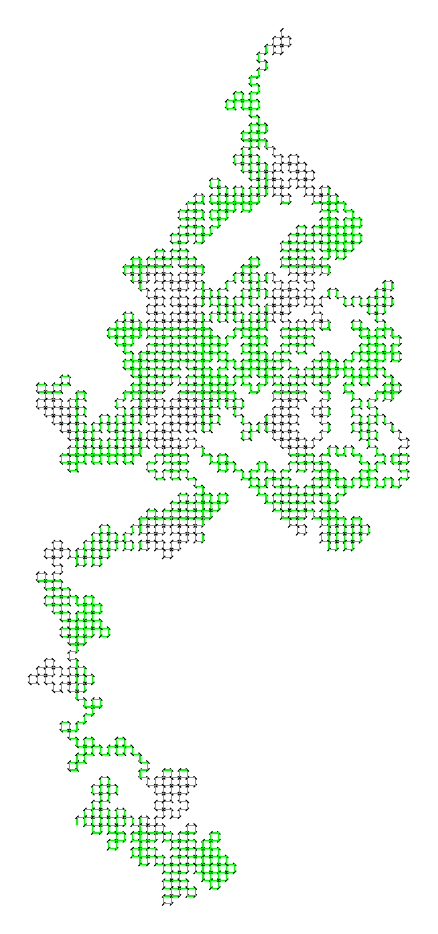
\begin{tikzpicture}
    [scale=0.1,only marks,reddot/.style={fill=red,circle,inner sep=1pt, minimum width=0.5pt},bluedot/.style={fill=blue,circle, inner sep=2pt, minimum width=0.5pt},
    blackdot/.style={fill=black,circle, inner sep=2pt, minimum width=0.5pt},
    yellowdot/.style={fill=yellow,circle, inner sep=2pt, minimum width=0.5pt},
    greendot/.style={fill=green,circle, inner sep=2pt, minimum width=0.5pt},    
     %using the 'spy' to magnify a part of the picture
     spy using outlines={rectangle,lens={scale=3}, size=6cm, connect spies},
     %using the decoration 'brace' (=a curly brace as path replacement)
     %decoration={brace,amplitude=2pt}
]

\draw[color=green] (0,0) -- (0,1);\draw[color=black] (0.2,1.2) -- (-0.2,0.8);
\draw[color=green] (0,1) -- (1,1);\draw[color=black] (1.2,1.2) -- (0.8,0.8);
\draw[color=green] (1,1) -- (1,2);\draw[color=black] (1.2,2.2) -- (0.8,1.8);
\draw[color=green] (1,2) -- (2,2);\draw[color=black] (2.2,2.2) -- (1.8,1.8);
\draw[color=green] (2,2) -- (2,3);\draw[color=black] (2.2,3.2) -- (1.8,2.8);
\draw[color=green] (2,3) -- (3,3);\draw[color=black] (3.2,3.2) -- (2.8,2.8);
\draw[color=green] (3,3) -- (3,4);\draw[color=black] (2.8,4.2) -- (3.2,3.8);
\draw[color=green] (3,4) -- (2,4);\draw[color=black] (1.8,4.2) -- (2.2,3.8);
\draw[color=green] (2,4) -- (2,5);\draw[color=black] (2.2,5.2) -- (1.8,4.8);
\draw[color=green] (2,5) -- (3,5);\draw[color=black] (3.2,5.2) -- (2.8,4.8);
\draw[color=green] (3,5) -- (3,6);\draw[color=black] (3.2,6.2) -- (2.8,5.8);
\draw[color=green] (3,6) -- (4,6);\draw[color=black] (3.8,6.2) -- (4.2,5.8);
\draw[color=green] (4,6) -- (4,5);\draw[color=black] (4.2,5.2) -- (3.8,4.8);
\draw[color=green] (4,5) -- (5,5);\draw[color=black] (4.8,5.2) -- (5.2,4.8);
\draw[color=green] (5,5) -- (5,4);\draw[color=black] (4.8,4.2) -- (5.2,3.8);
\draw[color=green] (5,4) -- (4,4);\draw[color=black] (3.8,4.2) -- (4.2,3.8);
\draw[color=green] (4,4) -- (4,5);\draw[color=black] (3.8,5.2) -- (4.2,4.8);
\draw[color=green] (4,5) -- (3,5);\draw[color=black] (3.2,5.2) -- (2.8,4.8);
\draw[color=green] (3,5) -- (3,4);\draw[color=black] (3.2,4.2) -- (2.8,3.8);
\draw[color=green] (3,4) -- (4,4);\draw[color=black] (3.8,4.2) -- (4.2,3.8);
\draw[color=green] (4,4) -- (4,3);\draw[color=black] (3.8,3.2) -- (4.2,2.8);
\draw[color=green] (4,3) -- (3,3);\draw[color=black] (3.2,3.2) -- (2.8,2.8);
\draw[color=green] (3,3) -- (3,2);\draw[color=black] (2.8,2.2) -- (3.2,1.8);
\draw[color=green] (3,2) -- (2,2);\draw[color=black] (2.2,2.2) -- (1.8,1.8);
\draw[color=green] (2,2) -- (2,1);\draw[color=black] (1.8,1.2) -- (2.2,0.8);
\draw[color=green] (2,1) -- (1,1);\draw[color=black] (1.2,1.2) -- (0.8,0.8);
\draw[color=green] (1,1) -- (1,0);\draw[color=black] (1.2,0.2) -- (0.8,-0.2);
\draw[color=green] (1,0) -- (2,0);\draw[color=black] (1.8,0.2) -- (2.2,-0.2);
\draw[color=green] (2,0) -- (2,-1);\draw[color=black] (2.2,-0.8) -- (1.8,-1.2);
\draw[color=green] (2,-1) -- (3,-1);\draw[color=black] (3.2,-0.8) -- (2.8,-1.2);
\draw[color=green] (3,-1) -- (3,0);\draw[color=black] (2.8,0.2) -- (3.2,-0.2);
\draw[color=green] (3,0) -- (2,0);\draw[color=black] (1.8,0.2) -- (2.2,-0.2);
\draw[color=green] (2,0) -- (2,1);\draw[color=black] (2.2,1.2) -- (1.8,0.8);
\draw[color=green] (2,1) -- (3,1);\draw[color=black] (2.8,1.2) -- (3.2,0.8);
\draw[color=green] (3,1) -- (3,0);\draw[color=black] (3.2,0.2) -- (2.8,-0.2);
\draw[color=green] (3,0) -- (4,0);\draw[color=black] (3.8,0.2) -- (4.2,-0.2);
\draw[color=green] (4,0) -- (4,-1);\draw[color=black] (4.2,-0.8) -- (3.8,-1.2);
\draw[color=green] (4,-1) -- (5,-1);\draw[color=black] (4.8,-0.8) -- (5.2,-1.2);
\draw[color=green] (5,-1) -- (5,-2);\draw[color=black] (4.8,-1.8) -- (5.2,-2.2);
\draw[color=green] (5,-2) -- (4,-2);\draw[color=black] (4.2,-1.8) -- (3.8,-2.2);
\draw[color=green] (4,-2) -- (4,-3);\draw[color=black] (4.2,-2.8) -- (3.8,-3.2);
\draw[color=green] (4,-3) -- (5,-3);\draw[color=black] (5.2,-2.8) -- (4.8,-3.2);
\draw[color=green] (5,-3) -- (5,-2);\draw[color=black] (5.2,-1.8) -- (4.8,-2.2);
\draw[color=green] (5,-2) -- (6,-2);\draw[color=black] (6.2,-1.8) -- (5.8,-2.2);
\draw[color=green] (6,-2) -- (6,-1);\draw[color=black] (5.8,-0.8) -- (6.2,-1.2);
\draw[color=green] (6,-1) -- (5,-1);\draw[color=black] (4.8,-0.8) -- (5.2,-1.2);
\draw[color=green] (5,-1) -- (5,0);\draw[color=black] (5.2,0.2) -- (4.8,-0.2);
\draw[color=green] (5,0) -- (6,0);\draw[color=black] (6.2,0.2) -- (5.8,-0.2);
\draw[color=green] (6,0) -- (6,1);\draw[color=black] (5.8,1.2) -- (6.2,0.8);
\draw[color=green] (6,1) -- (5,1);\draw[color=black] (5.2,1.2) -- (4.8,0.8);
\draw[color=green] (5,1) -- (5,0);\draw[color=black] (4.8,0.2) -- (5.2,-0.2);
\draw[color=green] (5,0) -- (4,0);\draw[color=black] (3.8,0.2) -- (4.2,-0.2);
\draw[color=green] (4,0) -- (4,1);\draw[color=black] (3.8,1.2) -- (4.2,0.8);
\draw[color=green] (4,1) -- (3,1);\draw[color=black] (2.8,1.2) -- (3.2,0.8);
\draw[color=green] (3,1) -- (3,2);\draw[color=black] (3.2,2.2) -- (2.8,1.8);
\draw[color=green] (3,2) -- (4,2);\draw[color=black] (3.8,2.2) -- (4.2,1.8);
\draw[color=green] (4,2) -- (4,1);\draw[color=black] (4.2,1.2) -- (3.8,0.8);
\draw[color=green] (4,1) -- (5,1);\draw[color=black] (5.2,1.2) -- (4.8,0.8);
\draw[color=green] (5,1) -- (5,2);\draw[color=black] (5.2,2.2) -- (4.8,1.8);
\draw[color=green] (5,2) -- (6,2);\draw[color=black] (5.8,2.2) -- (6.2,1.8);
\draw[color=green] (6,2) -- (6,1);\draw[color=black] (6.2,1.2) -- (5.8,0.8);
\draw[color=green] (6,1) -- (7,1);\draw[color=black] (6.8,1.2) -- (7.2,0.8);
\draw[color=green] (7,1) -- (7,0);\draw[color=black] (7.2,0.2) -- (6.8,-0.2);
\draw[color=green] (7,0) -- (8,0);\draw[color=black] (8.2,0.2) -- (7.8,-0.2);
\draw[color=green] (8,0) -- (8,1);\draw[color=black] (8.2,1.2) -- (7.8,0.8);
\draw[color=green] (8,1) -- (9,1);\draw[color=black] (8.8,1.2) -- (9.2,0.8);
\draw[color=green] (9,1) -- (9,0);\draw[color=black] (8.8,0.2) -- (9.2,-0.2);
\draw[color=green] (9,0) -- (8,0);\draw[color=black] (8.2,0.2) -- (7.8,-0.2);
\draw[color=green] (8,0) -- (8,-1);\draw[color=black] (7.8,-0.8) -- (8.2,-1.2);
\draw[color=green] (8,-1) -- (7,-1);\draw[color=black] (7.2,-0.8) -- (6.8,-1.2);
\draw[color=green] (7,-1) -- (7,-2);\draw[color=black] (7.2,-1.8) -- (6.8,-2.2);
\draw[color=green] (7,-2) -- (8,-2);\draw[color=black] (7.8,-1.8) -- (8.2,-2.2);
\draw[color=green] (8,-2) -- (8,-3);\draw[color=black] (7.8,-2.8) -- (8.2,-3.2);
\draw[color=green] (8,-3) -- (7,-3);\draw[color=black] (7.2,-2.8) -- (6.8,-3.2);
\draw[color=green] (7,-3) -- (7,-4);\draw[color=black] (7.2,-3.8) -- (6.8,-4.2);
\draw[color=green] (7,-4) -- (8,-4);\draw[color=black] (7.8,-3.8) -- (8.2,-4.2);
\draw[color=green] (8,-4) -- (8,-5);\draw[color=black] (8.2,-4.8) -- (7.8,-5.2);
\draw[color=green] (8,-5) -- (9,-5);\draw[color=black] (9.2,-4.8) -- (8.8,-5.2);
\draw[color=green] (9,-5) -- (9,-4);\draw[color=black] (8.8,-3.8) -- (9.2,-4.2);
\draw[color=green] (9,-4) -- (8,-4);\draw[color=black] (7.8,-3.8) -- (8.2,-4.2);
\draw[color=green] (8,-4) -- (8,-3);\draw[color=black] (8.2,-2.8) -- (7.8,-3.2);
\draw[color=green] (8,-3) -- (9,-3);\draw[color=black] (9.2,-2.8) -- (8.8,-3.2);
\draw[color=green] (9,-3) -- (9,-2);\draw[color=black] (8.8,-1.8) -- (9.2,-2.2);
\draw[color=green] (9,-2) -- (8,-2);\draw[color=black] (7.8,-1.8) -- (8.2,-2.2);
\draw[color=green] (8,-2) -- (8,-1);\draw[color=black] (8.2,-0.8) -- (7.8,-1.2);
\draw[color=green] (8,-1) -- (9,-1);\draw[color=black] (8.8,-0.8) -- (9.2,-1.2);
\draw[color=green] (9,-1) -- (9,-2);\draw[color=black] (9.2,-1.8) -- (8.8,-2.2);
\draw[color=green] (9,-2) -- (10,-2);\draw[color=black] (10.2,-1.8) -- (9.8,-2.2);
\draw[color=green] (10,-2) -- (10,-1);\draw[color=black] (10.2,-0.8) -- (9.8,-1.2);
\draw[color=green] (10,-1) -- (11,-1);\draw[color=black] (10.8,-0.8) -- (11.2,-1.2);
\draw[color=green] (11,-1) -- (11,-2);\draw[color=black] (11.2,-1.8) -- (10.8,-2.2);
\draw[color=green] (11,-2) -- (12,-2);\draw[color=black] (11.8,-1.8) -- (12.2,-2.2);
\draw[color=green] (12,-2) -- (12,-3);\draw[color=black] (12.2,-2.8) -- (11.8,-3.2);
\draw[color=green] (12,-3) -- (13,-3);\draw[color=black] (12.8,-2.8) -- (13.2,-3.2);
\draw[color=green] (13,-3) -- (13,-4);\draw[color=black] (12.8,-3.8) -- (13.2,-4.2);
\draw[color=green] (13,-4) -- (12,-4);\draw[color=black] (12.2,-3.8) -- (11.8,-4.2);
\draw[color=green] (12,-4) -- (12,-5);\draw[color=black] (11.8,-4.8) -- (12.2,-5.2);
\draw[color=green] (12,-5) -- (11,-5);\draw[color=black] (10.8,-4.8) -- (11.2,-5.2);
\draw[color=green] (11,-5) -- (11,-4);\draw[color=black] (10.8,-3.8) -- (11.2,-4.2);
\draw[color=green] (11,-4) -- (10,-4);\draw[color=black] (9.8,-3.8) -- (10.2,-4.2);
\draw[color=green] (10,-4) -- (10,-3);\draw[color=black] (9.8,-2.8) -- (10.2,-3.2);
\draw[color=green] (10,-3) -- (9,-3);\draw[color=black] (9.2,-2.8) -- (8.8,-3.2);
\draw[color=green] (9,-3) -- (9,-4);\draw[color=black] (9.2,-3.8) -- (8.8,-4.2);
\draw[color=green] (9,-4) -- (10,-4);\draw[color=black] (9.8,-3.8) -- (10.2,-4.2);
\draw[color=green] (10,-4) -- (10,-5);\draw[color=black] (10.2,-4.8) -- (9.8,-5.2);
\draw[color=green] (10,-5) -- (11,-5);\draw[color=black] (10.8,-4.8) -- (11.2,-5.2);
\draw[color=green] (11,-5) -- (11,-6);\draw[color=black] (11.2,-5.8) -- (10.8,-6.2);
\draw[color=green] (11,-6) -- (12,-6);\draw[color=black] (12.2,-5.8) -- (11.8,-6.2);
\draw[color=green] (12,-6) -- (12,-5);\draw[color=black] (12.2,-4.8) -- (11.8,-5.2);
\draw[color=green] (12,-5) -- (13,-5);\draw[color=black] (13.2,-4.8) -- (12.8,-5.2);
\draw[color=green] (13,-5) -- (13,-4);\draw[color=black] (13.2,-3.8) -- (12.8,-4.2);
\draw[color=green] (13,-4) -- (14,-4);\draw[color=black] (13.8,-3.8) -- (14.2,-4.2);
\draw[color=green] (14,-4) -- (14,-5);\draw[color=black] (13.8,-4.8) -- (14.2,-5.2);
\draw[color=green] (14,-5) -- (13,-5);\draw[color=black] (13.2,-4.8) -- (12.8,-5.2);
\draw[color=green] (13,-5) -- (13,-6);\draw[color=black] (12.8,-5.8) -- (13.2,-6.2);
\draw[color=green] (13,-6) -- (12,-6);\draw[color=black] (12.2,-5.8) -- (11.8,-6.2);
\draw[color=green] (12,-6) -- (12,-7);\draw[color=black] (11.8,-6.8) -- (12.2,-7.2);
\draw[color=green] (12,-7) -- (11,-7);\draw[color=black] (11.2,-6.8) -- (10.8,-7.2);
\draw[color=green] (11,-7) -- (11,-8);\draw[color=black] (11.2,-7.8) -- (10.8,-8.2);
\draw[color=green] (11,-8) -- (12,-8);\draw[color=black] (12.2,-7.8) -- (11.8,-8.2);
\draw[color=green] (12,-8) -- (12,-7);\draw[color=black] (12.2,-6.8) -- (11.8,-7.2);
\draw[color=green] (12,-7) -- (13,-7);\draw[color=black] (12.8,-6.8) -- (13.2,-7.2);
\draw[color=green] (13,-7) -- (13,-8);\draw[color=black] (12.8,-7.8) -- (13.2,-8.2);
\draw[color=green] (13,-8) -- (12,-8);\draw[color=black] (12.2,-7.8) -- (11.8,-8.2);
\draw[color=green] (12,-8) -- (12,-9);\draw[color=black] (11.8,-8.8) -- (12.2,-9.2);
\draw[color=green] (12,-9) -- (11,-9);\draw[color=black] (11.2,-8.8) -- (10.8,-9.2);
\draw[color=green] (11,-9) -- (11,-10);\draw[color=black] (11.2,-9.8) -- (10.8,-10.2);
\draw[color=green] (11,-10) -- (12,-10);\draw[color=black] (12.2,-9.8) -- (11.8,-10.2);
\draw[color=green] (12,-10) -- (12,-9);\draw[color=black] (12.2,-8.8) -- (11.8,-9.2);
\draw[color=green] (12,-9) -- (13,-9);\draw[color=black] (13.2,-8.8) -- (12.8,-9.2);
\draw[color=green] (13,-9) -- (13,-8);\draw[color=black] (13.2,-7.8) -- (12.8,-8.2);
\draw[color=green] (13,-8) -- (14,-8);\draw[color=black] (13.8,-7.8) -- (14.2,-8.2);
\draw[color=green] (14,-8) -- (14,-9);\draw[color=black] (14.2,-8.8) -- (13.8,-9.2);
\draw[color=green] (14,-9) -- (15,-9);\draw[color=black] (15.2,-8.8) -- (14.8,-9.2);
\draw[color=green] (15,-9) -- (15,-8);\draw[color=black] (14.8,-7.8) -- (15.2,-8.2);
\draw[color=green] (15,-8) -- (14,-8);\draw[color=black] (13.8,-7.8) -- (14.2,-8.2);
\draw[color=green] (14,-8) -- (14,-7);\draw[color=black] (13.8,-6.8) -- (14.2,-7.2);
\draw[color=green] (14,-7) -- (13,-7);\draw[color=black] (12.8,-6.8) -- (13.2,-7.2);
\draw[color=green] (13,-7) -- (13,-6);\draw[color=black] (13.2,-5.8) -- (12.8,-6.2);
\draw[color=green] (13,-6) -- (14,-6);\draw[color=black] (14.2,-5.8) -- (13.8,-6.2);
\draw[color=green] (14,-6) -- (14,-5);\draw[color=black] (14.2,-4.8) -- (13.8,-5.2);
\draw[color=green] (14,-5) -- (15,-5);\draw[color=black] (14.8,-4.8) -- (15.2,-5.2);
\draw[color=green] (15,-5) -- (15,-6);\draw[color=black] (15.2,-5.8) -- (14.8,-6.2);
\draw[color=green] (15,-6) -- (16,-6);\draw[color=black] (15.8,-5.8) -- (16.2,-6.2);
\draw[color=green] (16,-6) -- (16,-7);\draw[color=black] (16.2,-6.8) -- (15.8,-7.2);
\draw[color=green] (16,-7) -- (17,-7);\draw[color=black] (17.2,-6.8) -- (16.8,-7.2);
\draw[color=green] (17,-7) -- (17,-6);\draw[color=black] (17.2,-5.8) -- (16.8,-6.2);
\draw[color=green] (17,-6) -- (18,-6);\draw[color=black] (18.2,-5.8) -- (17.8,-6.2);
\draw[color=green] (18,-6) -- (18,-5);\draw[color=black] (17.8,-4.8) -- (18.2,-5.2);
\draw[color=green] (18,-5) -- (17,-5);\draw[color=black] (17.2,-4.8) -- (16.8,-5.2);
\draw[color=green] (17,-5) -- (17,-6);\draw[color=black] (16.8,-5.8) -- (17.2,-6.2);
\draw[color=green] (17,-6) -- (16,-6);\draw[color=black] (15.8,-5.8) -- (16.2,-6.2);
\draw[color=green] (16,-6) -- (16,-5);\draw[color=black] (15.8,-4.8) -- (16.2,-5.2);
\draw[color=green] (16,-5) -- (15,-5);\draw[color=black] (14.8,-4.8) -- (15.2,-5.2);
\draw[color=green] (15,-5) -- (15,-4);\draw[color=black] (15.2,-3.8) -- (14.8,-4.2);
\draw[color=green] (15,-4) -- (16,-4);\draw[color=black] (16.2,-3.8) -- (15.8,-4.2);
\draw[color=green] (16,-4) -- (16,-3);\draw[color=black] (16.2,-2.8) -- (15.8,-3.2);
\draw[color=green] (16,-3) -- (17,-3);\draw[color=black] (16.8,-2.8) -- (17.2,-3.2);
\draw[color=green] (17,-3) -- (17,-4);\draw[color=black] (16.8,-3.8) -- (17.2,-4.2);
\draw[color=green] (17,-4) -- (16,-4);\draw[color=black] (16.2,-3.8) -- (15.8,-4.2);
\draw[color=green] (16,-4) -- (16,-5);\draw[color=black] (16.2,-4.8) -- (15.8,-5.2);
\draw[color=green] (16,-5) -- (17,-5);\draw[color=black] (17.2,-4.8) -- (16.8,-5.2);
\draw[color=green] (17,-5) -- (17,-4);\draw[color=black] (17.2,-3.8) -- (16.8,-4.2);
\draw[color=green] (17,-4) -- (18,-4);\draw[color=black] (17.8,-3.8) -- (18.2,-4.2);
\draw[color=green] (18,-4) -- (18,-5);\draw[color=black] (18.2,-4.8) -- (17.8,-5.2);
\draw[color=green] (18,-5) -- (19,-5);\draw[color=black] (18.8,-4.8) -- (19.2,-5.2);
\draw[color=green] (19,-5) -- (19,-6);\draw[color=black] (18.8,-5.8) -- (19.2,-6.2);
\draw[color=green] (19,-6) -- (18,-6);\draw[color=black] (18.2,-5.8) -- (17.8,-6.2);
\draw[color=green] (18,-6) -- (18,-7);\draw[color=black] (17.8,-6.8) -- (18.2,-7.2);
\draw[color=green] (18,-7) -- (17,-7);\draw[color=black] (17.2,-6.8) -- (16.8,-7.2);
\draw[color=green] (17,-7) -- (17,-8);\draw[color=black] (17.2,-7.8) -- (16.8,-8.2);
\draw[color=green] (17,-8) -- (18,-8);\draw[color=black] (18.2,-7.8) -- (17.8,-8.2);
\draw[color=green] (18,-8) -- (18,-7);\draw[color=black] (18.2,-6.8) -- (17.8,-7.2);
\draw[color=green] (18,-7) -- (19,-7);\draw[color=black] (19.2,-6.8) -- (18.8,-7.2);
\draw[color=green] (19,-7) -- (19,-6);\draw[color=black] (19.2,-5.8) -- (18.8,-6.2);
\draw[color=green] (19,-6) -- (20,-6);\draw[color=black] (20.2,-5.8) -- (19.8,-6.2);
\draw[color=green] (20,-6) -- (20,-5);\draw[color=black] (19.8,-4.8) -- (20.2,-5.2);
\draw[color=green] (20,-5) -- (19,-5);\draw[color=black] (18.8,-4.8) -- (19.2,-5.2);
\draw[color=green] (19,-5) -- (19,-4);\draw[color=black] (18.8,-3.8) -- (19.2,-4.2);
\draw[color=green] (19,-4) -- (18,-4);\draw[color=black] (17.8,-3.8) -- (18.2,-4.2);
\draw[color=green] (18,-4) -- (18,-3);\draw[color=black] (17.8,-2.8) -- (18.2,-3.2);
\draw[color=green] (18,-3) -- (17,-3);\draw[color=black] (16.8,-2.8) -- (17.2,-3.2);
\draw[color=green] (17,-3) -- (17,-2);\draw[color=black] (17.2,-1.8) -- (16.8,-2.2);
\draw[color=green] (17,-2) -- (18,-2);\draw[color=black] (18.2,-1.8) -- (17.8,-2.2);
\draw[color=green] (18,-2) -- (18,-1);\draw[color=black] (17.8,-0.8) -- (18.2,-1.2);
\draw[color=green] (18,-1) -- (17,-1);\draw[color=black] (17.2,-0.8) -- (16.8,-1.2);
\draw[color=green] (17,-1) -- (17,-2);\draw[color=black] (16.8,-1.8) -- (17.2,-2.2);
\draw[color=green] (17,-2) -- (16,-2);\draw[color=black] (16.2,-1.8) -- (15.8,-2.2);
\draw[color=green] (16,-2) -- (16,-3);\draw[color=black] (15.8,-2.8) -- (16.2,-3.2);
\draw[color=green] (16,-3) -- (15,-3);\draw[color=black] (14.8,-2.8) -- (15.2,-3.2);
\draw[color=green] (15,-3) -- (15,-2);\draw[color=black] (14.8,-1.8) -- (15.2,-2.2);
\draw[color=green] (15,-2) -- (14,-2);\draw[color=black] (14.2,-1.8) -- (13.8,-2.2);
\draw[color=green] (14,-2) -- (14,-3);\draw[color=black] (14.2,-2.8) -- (13.8,-3.2);
\draw[color=green] (14,-3) -- (15,-3);\draw[color=black] (14.8,-2.8) -- (15.2,-3.2);
\draw[color=green] (15,-3) -- (15,-4);\draw[color=black] (14.8,-3.8) -- (15.2,-4.2);
\draw[color=green] (15,-4) -- (14,-4);\draw[color=black] (13.8,-3.8) -- (14.2,-4.2);
\draw[color=green] (14,-4) -- (14,-3);\draw[color=black] (13.8,-2.8) -- (14.2,-3.2);
\draw[color=green] (14,-3) -- (13,-3);\draw[color=black] (12.8,-2.8) -- (13.2,-3.2);
\draw[color=green] (13,-3) -- (13,-2);\draw[color=black] (13.2,-1.8) -- (12.8,-2.2);
\draw[color=green] (13,-2) -- (14,-2);\draw[color=black] (14.2,-1.8) -- (13.8,-2.2);
\draw[color=green] (14,-2) -- (14,-1);\draw[color=black] (14.2,-0.8) -- (13.8,-1.2);
\draw[color=green] (14,-1) -- (15,-1);\draw[color=black] (15.2,-0.8) -- (14.8,-1.2);
\draw[color=green] (15,-1) -- (15,0);\draw[color=black] (14.8,0.2) -- (15.2,-0.2);
\draw[color=green] (15,0) -- (14,0);\draw[color=black] (14.2,0.2) -- (13.8,-0.2);
\draw[color=green] (14,0) -- (14,-1);\draw[color=black] (13.8,-0.8) -- (14.2,-1.2);
\draw[color=green] (14,-1) -- (13,-1);\draw[color=black] (13.2,-0.8) -- (12.8,-1.2);
\draw[color=green] (13,-1) -- (13,-2);\draw[color=black] (12.8,-1.8) -- (13.2,-2.2);
\draw[color=green] (13,-2) -- (12,-2);\draw[color=black] (11.8,-1.8) -- (12.2,-2.2);
\draw[color=green] (12,-2) -- (12,-1);\draw[color=black] (11.8,-0.8) -- (12.2,-1.2);
\draw[color=green] (12,-1) -- (11,-1);\draw[color=black] (10.8,-0.8) -- (11.2,-1.2);
\draw[color=green] (11,-1) -- (11,0);\draw[color=black] (10.8,0.2) -- (11.2,-0.2);
\draw[color=green] (11,0) -- (10,0);\draw[color=black] (10.2,0.2) -- (9.8,-0.2);
\draw[color=green] (10,0) -- (10,-1);\draw[color=black] (9.8,-0.8) -- (10.2,-1.2);
\draw[color=green] (10,-1) -- (9,-1);\draw[color=black] (8.8,-0.8) -- (9.2,-1.2);
\draw[color=green] (9,-1) -- (9,0);\draw[color=black] (9.2,0.2) -- (8.8,-0.2);
\draw[color=green] (9,0) -- (10,0);\draw[color=black] (10.2,0.2) -- (9.8,-0.2);
\draw[color=green] (10,0) -- (10,1);\draw[color=black] (10.2,1.2) -- (9.8,0.8);
\draw[color=green] (10,1) -- (11,1);\draw[color=black] (11.2,1.2) -- (10.8,0.8);
\draw[color=green] (11,1) -- (11,2);\draw[color=black] (10.8,2.2) -- (11.2,1.8);
\draw[color=green] (11,2) -- (10,2);\draw[color=black] (9.8,2.2) -- (10.2,1.8);
\draw[color=green] (10,2) -- (10,3);\draw[color=black] (10.2,3.2) -- (9.8,2.8);
\draw[color=green] (10,3) -- (11,3);\draw[color=black] (11.2,3.2) -- (10.8,2.8);
\draw[color=green] (11,3) -- (11,4);\draw[color=black] (11.2,4.2) -- (10.8,3.8);
\draw[color=green] (11,4) -- (12,4);\draw[color=black] (11.8,4.2) -- (12.2,3.8);
\draw[color=green] (12,4) -- (12,3);\draw[color=black] (11.8,3.2) -- (12.2,2.8);
\draw[color=green] (12,3) -- (11,3);\draw[color=black] (11.2,3.2) -- (10.8,2.8);
\draw[color=green] (11,3) -- (11,2);\draw[color=black] (11.2,2.2) -- (10.8,1.8);
\draw[color=green] (11,2) -- (12,2);\draw[color=black] (11.8,2.2) -- (12.2,1.8);
\draw[color=green] (12,2) -- (12,1);\draw[color=black] (12.2,1.2) -- (11.8,0.8);
\draw[color=green] (12,1) -- (13,1);\draw[color=black] (13.2,1.2) -- (12.8,0.8);
\draw[color=green] (13,1) -- (13,2);\draw[color=black] (13.2,2.2) -- (12.8,1.8);
\draw[color=green] (13,2) -- (14,2);\draw[color=black] (14.2,2.2) -- (13.8,1.8);
\draw[color=green] (14,2) -- (14,3);\draw[color=black] (13.8,3.2) -- (14.2,2.8);
\draw[color=green] (14,3) -- (13,3);\draw[color=black] (12.8,3.2) -- (13.2,2.8);
\draw[color=green] (13,3) -- (13,4);\draw[color=black] (12.8,4.2) -- (13.2,3.8);
\draw[color=green] (13,4) -- (12,4);\draw[color=black] (11.8,4.2) -- (12.2,3.8);
\draw[color=green] (12,4) -- (12,5);\draw[color=black] (11.8,5.2) -- (12.2,4.8);
\draw[color=green] (12,5) -- (11,5);\draw[color=black] (10.8,5.2) -- (11.2,4.8);
\draw[color=green] (11,5) -- (11,6);\draw[color=black] (11.2,6.2) -- (10.8,5.8);
\draw[color=green] (11,6) -- (12,6);\draw[color=black] (11.8,6.2) -- (12.2,5.8);
\draw[color=green] (12,6) -- (12,5);\draw[color=black] (12.2,5.2) -- (11.8,4.8);
\draw[color=green] (12,5) -- (13,5);\draw[color=black] (12.8,5.2) -- (13.2,4.8);
\draw[color=green] (13,5) -- (13,4);\draw[color=black] (13.2,4.2) -- (12.8,3.8);
\draw[color=green] (13,4) -- (14,4);\draw[color=black] (14.2,4.2) -- (13.8,3.8);
\draw[color=green] (14,4) -- (14,5);\draw[color=black] (14.2,5.2) -- (13.8,4.8);
\draw[color=green] (14,5) -- (15,5);\draw[color=black] (15.2,5.2) -- (14.8,4.8);
\draw[color=green] (15,5) -- (15,6);\draw[color=black] (14.8,6.2) -- (15.2,5.8);
\draw[color=green] (15,6) -- (14,6);\draw[color=black] (14.2,6.2) -- (13.8,5.8);
\draw[color=green] (14,6) -- (14,5);\draw[color=black] (13.8,5.2) -- (14.2,4.8);
\draw[color=green] (14,5) -- (13,5);\draw[color=black] (12.8,5.2) -- (13.2,4.8);
\draw[color=green] (13,5) -- (13,6);\draw[color=black] (13.2,6.2) -- (12.8,5.8);
\draw[color=green] (13,6) -- (14,6);\draw[color=black] (14.2,6.2) -- (13.8,5.8);
\draw[color=green] (14,6) -- (14,7);\draw[color=black] (13.8,7.2) -- (14.2,6.8);
\draw[color=green] (14,7) -- (13,7);\draw[color=black] (13.2,7.2) -- (12.8,6.8);
\draw[color=green] (13,7) -- (13,6);\draw[color=black] (12.8,6.2) -- (13.2,5.8);
\draw[color=green] (13,6) -- (12,6);\draw[color=black] (11.8,6.2) -- (12.2,5.8);
\draw[color=green] (12,6) -- (12,7);\draw[color=black] (11.8,7.2) -- (12.2,6.8);
\draw[color=green] (12,7) -- (11,7);\draw[color=black] (11.2,7.2) -- (10.8,6.8);
\draw[color=green] (11,7) -- (11,6);\draw[color=black] (10.8,6.2) -- (11.2,5.8);
\draw[color=green] (11,6) -- (10,6);\draw[color=black] (10.2,6.2) -- (9.8,5.8);
\draw[color=green] (10,6) -- (10,5);\draw[color=black] (10.2,5.2) -- (9.8,4.8);
\draw[color=green] (10,5) -- (11,5);\draw[color=black] (10.8,5.2) -- (11.2,4.8);
\draw[color=green] (11,5) -- (11,4);\draw[color=black] (10.8,4.2) -- (11.2,3.8);
\draw[color=green] (11,4) -- (10,4);\draw[color=black] (9.8,4.2) -- (10.2,3.8);
\draw[color=green] (10,4) -- (10,5);\draw[color=black] (9.8,5.2) -- (10.2,4.8);
\draw[color=green] (10,5) -- (9,5);\draw[color=black] (8.8,5.2) -- (9.2,4.8);
\draw[color=green] (9,5) -- (9,6);\draw[color=black] (8.8,6.2) -- (9.2,5.8);
\draw[color=green] (9,6) -- (8,6);\draw[color=black] (7.8,6.2) -- (8.2,5.8);
\draw[color=green] (8,6) -- (8,7);\draw[color=black] (8.2,7.2) -- (7.8,6.8);
\draw[color=green] (8,7) -- (9,7);\draw[color=black] (9.2,7.2) -- (8.8,6.8);
\draw[color=green] (9,7) -- (9,8);\draw[color=black] (8.8,8.2) -- (9.2,7.8);
\draw[color=green] (9,8) -- (8,8);\draw[color=black] (7.8,8.2) -- (8.2,7.8);
\draw[color=green] (8,8) -- (8,9);\draw[color=black] (7.8,9.2) -- (8.2,8.8);
\draw[color=green] (8,9) -- (7,9);\draw[color=black] (6.8,9.2) -- (7.2,8.8);
\draw[color=green] (7,9) -- (7,10);\draw[color=black] (6.8,10.2) -- (7.2,9.8);
\draw[color=green] (7,10) -- (6,10);\draw[color=black] (5.8,10.2) -- (6.2,9.8);
\draw[color=green] (6,10) -- (6,11);\draw[color=black] (5.8,11.2) -- (6.2,10.8);
\draw[color=green] (6,11) -- (5,11);\draw[color=black] (5.2,11.2) -- (4.8,10.8);
\draw[color=green] (5,11) -- (5,10);\draw[color=black] (5.2,10.2) -- (4.8,9.8);
\draw[color=green] (5,10) -- (6,10);\draw[color=black] (5.8,10.2) -- (6.2,9.8);
\draw[color=green] (6,10) -- (6,9);\draw[color=black] (5.8,9.2) -- (6.2,8.8);
\draw[color=green] (6,9) -- (5,9);\draw[color=black] (4.8,9.2) -- (5.2,8.8);
\draw[color=green] (5,9) -- (5,10);\draw[color=black] (4.8,10.2) -- (5.2,9.8);
\draw[color=green] (5,10) -- (4,10);\draw[color=black] (4.2,10.2) -- (3.8,9.8);
\draw[color=green] (4,10) -- (4,9);\draw[color=black] (3.8,9.2) -- (4.2,8.8);
\draw[color=green] (4,9) -- (3,9);\draw[color=black] (2.8,9.2) -- (3.2,8.8);
\draw[color=green] (3,9) -- (3,10);\draw[color=black] (2.8,10.2) -- (3.2,9.8);
\draw[color=green] (3,10) -- (2,10);\draw[color=black] (2.2,10.2) -- (1.8,9.8);
\draw[color=green] (2,10) -- (2,9);\draw[color=black] (1.8,9.2) -- (2.2,8.8);
\draw[color=green] (2,9) -- (1,9);\draw[color=black] (1.2,9.2) -- (0.8,8.8);
\draw[color=green] (1,9) -- (1,8);\draw[color=black] (0.8,8.2) -- (1.2,7.8);
\draw[color=green] (1,8) -- (0,8);\draw[color=black] (0.2,8.2) -- (-0.2,7.8);
\draw[color=green] (0,8) -- (0,7);\draw[color=black] (-0.2,7.2) -- (0.2,6.8);
\draw[color=green] (0,7) -- (-1,7);\draw[color=black] (-1.2,7.2) -- (-0.8,6.8);
\draw[color=green] (-1,7) -- (-1,8);\draw[color=black] (-0.8,8.2) -- (-1.2,7.8);
\draw[color=green] (-1,8) -- (0,8);\draw[color=black] (0.2,8.2) -- (-0.2,7.8);
\draw[color=green] (0,8) -- (0,9);\draw[color=black] (0.2,9.2) -- (-0.2,8.8);
\draw[color=green] (0,9) -- (1,9);\draw[color=black] (1.2,9.2) -- (0.8,8.8);
\draw[color=green] (1,9) -- (1,10);\draw[color=black] (1.2,10.2) -- (0.8,9.8);
\draw[color=green] (1,10) -- (2,10);\draw[color=black] (2.2,10.2) -- (1.8,9.8);
\draw[color=green] (2,10) -- (2,11);\draw[color=black] (1.8,11.2) -- (2.2,10.8);
\draw[color=green] (2,11) -- (1,11);\draw[color=black] (1.2,11.2) -- (0.8,10.8);
\draw[color=green] (1,11) -- (1,10);\draw[color=black] (0.8,10.2) -- (1.2,9.8);
\draw[color=green] (1,10) -- (0,10);\draw[color=black] (-0.2,10.2) -- (0.2,9.8);
\draw[color=green] (0,10) -- (0,11);\draw[color=black] (-0.2,11.2) -- (0.2,10.8);
\draw[color=green] (0,11) -- (-1,11);\draw[color=black] (-1.2,11.2) -- (-0.8,10.8);
\draw[color=green] (-1,11) -- (-1,12);\draw[color=black] (-1.2,12.2) -- (-0.8,11.8);
\draw[color=green] (-1,12) -- (-2,12);\draw[color=black] (-2.2,12.2) -- (-1.8,11.8);
\draw[color=green] (-2,12) -- (-2,13);\draw[color=black] (-1.8,13.2) -- (-2.2,12.8);
\draw[color=green] (-2,13) -- (-1,13);\draw[color=black] (-1.2,13.2) -- (-0.8,12.8);
\draw[color=green] (-1,13) -- (-1,12);\draw[color=black] (-0.8,12.2) -- (-1.2,11.8);
\draw[color=green] (-1,12) -- (0,12);\draw[color=black] (0.2,12.2) -- (-0.2,11.8);
\draw[color=green] (0,12) -- (0,13);\draw[color=black] (0.2,13.2) -- (-0.2,12.8);
\draw[color=green] (0,13) -- (1,13);\draw[color=black] (1.2,13.2) -- (0.8,12.8);
\draw[color=green] (1,13) -- (1,14);\draw[color=black] (1.2,14.2) -- (0.8,13.8);
\draw[color=green] (1,14) -- (2,14);\draw[color=black] (2.2,14.2) -- (1.8,13.8);
\draw[color=green] (2,14) -- (2,15);\draw[color=black] (2.2,15.2) -- (1.8,14.8);
\draw[color=green] (2,15) -- (3,15);\draw[color=black] (3.2,15.2) -- (2.8,14.8);
\draw[color=green] (3,15) -- (3,16);\draw[color=black] (2.8,16.2) -- (3.2,15.8);
\draw[color=green] (3,16) -- (2,16);\draw[color=black] (2.2,16.2) -- (1.8,15.8);
\draw[color=green] (2,16) -- (2,15);\draw[color=black] (1.8,15.2) -- (2.2,14.8);
\draw[color=green] (2,15) -- (1,15);\draw[color=black] (0.8,15.2) -- (1.2,14.8);
\draw[color=green] (1,15) -- (1,16);\draw[color=black] (0.8,16.2) -- (1.2,15.8);
\draw[color=green] (1,16) -- (0,16);\draw[color=black] (-0.2,16.2) -- (0.2,15.8);
\draw[color=green] (0,16) -- (0,17);\draw[color=black] (0.2,17.2) -- (-0.2,16.8);
\draw[color=green] (0,17) -- (1,17);\draw[color=black] (1.2,17.2) -- (0.8,16.8);
\draw[color=green] (1,17) -- (1,18);\draw[color=black] (1.2,18.2) -- (0.8,17.8);
\draw[color=green] (1,18) -- (2,18);\draw[color=black] (2.2,18.2) -- (1.8,17.8);
\draw[color=green] (2,18) -- (2,19);\draw[color=black] (1.8,19.2) -- (2.2,18.8);
\draw[color=green] (2,19) -- (1,19);\draw[color=black] (0.8,19.2) -- (1.2,18.8);
\draw[color=green] (1,19) -- (1,20);\draw[color=black] (0.8,20.2) -- (1.2,19.8);
\draw[color=green] (1,20) -- (0,20);\draw[color=black] (0.2,20.2) -- (-0.2,19.8);
\draw[color=green] (0,20) -- (0,19);\draw[color=black] (0.2,19.2) -- (-0.2,18.8);
\draw[color=green] (0,19) -- (1,19);\draw[color=black] (0.8,19.2) -- (1.2,18.8);
\draw[color=green] (1,19) -- (1,18);\draw[color=black] (0.8,18.2) -- (1.2,17.8);
\draw[color=green] (1,18) -- (0,18);\draw[color=black] (-0.2,18.2) -- (0.2,17.8);
\draw[color=green] (0,18) -- (0,19);\draw[color=black] (-0.2,19.2) -- (0.2,18.8);
\draw[color=green] (0,19) -- (-1,19);\draw[color=black] (-0.8,19.2) -- (-1.2,18.8);
\draw[color=green] (-1,19) -- (-1,18);\draw[color=black] (-0.8,18.2) -- (-1.2,17.8);
\draw[color=green] (-1,18) -- (0,18);\draw[color=black] (-0.2,18.2) -- (0.2,17.8);
\draw[color=green] (0,18) -- (0,17);\draw[color=black] (-0.2,17.2) -- (0.2,16.8);
\draw[color=green] (0,17) -- (-1,17);\draw[color=black] (-1.2,17.2) -- (-0.8,16.8);
\draw[color=green] (-1,17) -- (-1,18);\draw[color=black] (-1.2,18.2) -- (-0.8,17.8);
\draw[color=green] (-1,18) -- (-2,18);\draw[color=black] (-1.8,18.2) -- (-2.2,17.8);
\draw[color=green] (-2,18) -- (-2,17);\draw[color=black] (-2.2,17.2) -- (-1.8,16.8);
\draw[color=green] (-2,17) -- (-3,17);\draw[color=black] (-3.2,17.2) -- (-2.8,16.8);
\draw[color=green] (-3,17) -- (-3,18);\draw[color=black] (-3.2,18.2) -- (-2.8,17.8);
\draw[color=green] (-3,18) -- (-4,18);\draw[color=black] (-4.2,18.2) -- (-3.8,17.8);
\draw[color=green] (-4,18) -- (-4,19);\draw[color=black] (-3.8,19.2) -- (-4.2,18.8);
\draw[color=green] (-4,19) -- (-3,19);\draw[color=black] (-2.8,19.2) -- (-3.2,18.8);
\draw[color=green] (-3,19) -- (-3,20);\draw[color=black] (-3.2,20.2) -- (-2.8,19.8);
\draw[color=green] (-3,20) -- (-4,20);\draw[color=black] (-3.8,20.2) -- (-4.2,19.8);
\draw[color=green] (-4,20) -- (-4,19);\draw[color=black] (-4.2,19.2) -- (-3.8,18.8);
\draw[color=green] (-4,19) -- (-5,19);\draw[color=black] (-4.8,19.2) -- (-5.2,18.8);
\draw[color=green] (-5,19) -- (-5,18);\draw[color=black] (-5.2,18.2) -- (-4.8,17.8);
\draw[color=green] (-5,18) -- (-6,18);\draw[color=black] (-6.2,18.2) -- (-5.8,17.8);
\draw[color=green] (-6,18) -- (-6,19);\draw[color=black] (-5.8,19.2) -- (-6.2,18.8);
\draw[color=green] (-6,19) -- (-5,19);\draw[color=black] (-4.8,19.2) -- (-5.2,18.8);
\draw[color=green] (-5,19) -- (-5,20);\draw[color=black] (-4.8,20.2) -- (-5.2,19.8);
\draw[color=green] (-5,20) -- (-4,20);\draw[color=black] (-3.8,20.2) -- (-4.2,19.8);
\draw[color=green] (-4,20) -- (-4,21);\draw[color=black] (-3.8,21.2) -- (-4.2,20.8);
\draw[color=green] (-4,21) -- (-3,21);\draw[color=black] (-3.2,21.2) -- (-2.8,20.8);
\draw[color=green] (-3,21) -- (-3,20);\draw[color=black] (-2.8,20.2) -- (-3.2,19.8);
\draw[color=green] (-3,20) -- (-2,20);\draw[color=black] (-2.2,20.2) -- (-1.8,19.8);
\draw[color=green] (-2,20) -- (-2,19);\draw[color=black] (-1.8,19.2) -- (-2.2,18.8);
\draw[color=green] (-2,19) -- (-1,19);\draw[color=black] (-0.8,19.2) -- (-1.2,18.8);
\draw[color=green] (-1,19) -- (-1,20);\draw[color=black] (-0.8,20.2) -- (-1.2,19.8);
\draw[color=green] (-1,20) -- (0,20);\draw[color=black] (0.2,20.2) -- (-0.2,19.8);
\draw[color=green] (0,20) -- (0,21);\draw[color=black] (-0.2,21.2) -- (0.2,20.8);
\draw[color=green] (0,21) -- (-1,21);\draw[color=black] (-1.2,21.2) -- (-0.8,20.8);
\draw[color=green] (-1,21) -- (-1,22);\draw[color=black] (-0.8,22.2) -- (-1.2,21.8);
\draw[color=green] (-1,22) -- (0,22);\draw[color=black] (0.2,22.2) -- (-0.2,21.8);
\draw[color=green] (0,22) -- (0,23);\draw[color=black] (0.2,23.2) -- (-0.2,22.8);
\draw[color=green] (0,23) -- (1,23);\draw[color=black] (1.2,23.2) -- (0.8,22.8);
\draw[color=green] (1,23) -- (1,24);\draw[color=black] (0.8,24.2) -- (1.2,23.8);
\draw[color=green] (1,24) -- (0,24);\draw[color=black] (0.2,24.2) -- (-0.2,23.8);
\draw[color=green] (0,24) -- (0,23);\draw[color=black] (-0.2,23.2) -- (0.2,22.8);
\draw[color=green] (0,23) -- (-1,23);\draw[color=black] (-1.2,23.2) -- (-0.8,22.8);
\draw[color=green] (-1,23) -- (-1,24);\draw[color=black] (-1.2,24.2) -- (-0.8,23.8);
\draw[color=green] (-1,24) -- (-2,24);\draw[color=black] (-2.2,24.2) -- (-1.8,23.8);
\draw[color=green] (-2,24) -- (-2,25);\draw[color=black] (-1.8,25.2) -- (-2.2,24.8);
\draw[color=green] (-2,25) -- (-1,25);\draw[color=black] (-1.2,25.2) -- (-0.8,24.8);
\draw[color=green] (-1,25) -- (-1,24);\draw[color=black] (-0.8,24.2) -- (-1.2,23.8);
\draw[color=green] (-1,24) -- (0,24);\draw[color=black] (0.2,24.2) -- (-0.2,23.8);
\draw[color=green] (0,24) -- (0,25);\draw[color=black] (0.2,25.2) -- (-0.2,24.8);
\draw[color=green] (0,25) -- (1,25);\draw[color=black] (1.2,25.2) -- (0.8,24.8);
\draw[color=green] (1,25) -- (1,26);\draw[color=black] (0.8,26.2) -- (1.2,25.8);
\draw[color=green] (1,26) -- (0,26);\draw[color=black] (0.2,26.2) -- (-0.2,25.8);
\draw[color=green] (0,26) -- (0,25);\draw[color=black] (-0.2,25.2) -- (0.2,24.8);
\draw[color=green] (0,25) -- (-1,25);\draw[color=black] (-1.2,25.2) -- (-0.8,24.8);
\draw[color=green] (-1,25) -- (-1,26);\draw[color=black] (-1.2,26.2) -- (-0.8,25.8);
\draw[color=green] (-1,26) -- (-2,26);\draw[color=black] (-2.2,26.2) -- (-1.8,25.8);
\draw[color=green] (-2,26) -- (-2,27);\draw[color=black] (-1.8,27.2) -- (-2.2,26.8);
\draw[color=green] (-2,27) -- (-1,27);\draw[color=black] (-1.2,27.2) -- (-0.8,26.8);
\draw[color=green] (-1,27) -- (-1,26);\draw[color=black] (-0.8,26.2) -- (-1.2,25.8);
\draw[color=green] (-1,26) -- (0,26);\draw[color=black] (0.2,26.2) -- (-0.2,25.8);
\draw[color=green] (0,26) -- (0,27);\draw[color=black] (0.2,27.2) -- (-0.2,26.8);
\draw[color=green] (0,27) -- (1,27);\draw[color=black] (0.8,27.2) -- (1.2,26.8);
\draw[color=green] (1,27) -- (1,26);\draw[color=black] (1.2,26.2) -- (0.8,25.8);
\draw[color=green] (1,26) -- (2,26);\draw[color=black] (1.8,26.2) -- (2.2,25.8);
\draw[color=green] (2,26) -- (2,25);\draw[color=black] (1.8,25.2) -- (2.2,24.8);
\draw[color=green] (2,25) -- (1,25);\draw[color=black] (1.2,25.2) -- (0.8,24.8);
\draw[color=green] (1,25) -- (1,24);\draw[color=black] (1.2,24.2) -- (0.8,23.8);
\draw[color=green] (1,24) -- (2,24);\draw[color=black] (2.2,24.2) -- (1.8,23.8);
\draw[color=green] (2,24) -- (2,25);\draw[color=black] (2.2,25.2) -- (1.8,24.8);
\draw[color=green] (2,25) -- (3,25);\draw[color=black] (2.8,25.2) -- (3.2,24.8);
\draw[color=green] (3,25) -- (3,24);\draw[color=black] (3.2,24.2) -- (2.8,23.8);
\draw[color=green] (3,24) -- (4,24);\draw[color=black] (4.2,24.2) -- (3.8,23.8);
\draw[color=green] (4,24) -- (4,25);\draw[color=black] (3.8,25.2) -- (4.2,24.8);
\draw[color=green] (4,25) -- (3,25);\draw[color=black] (2.8,25.2) -- (3.2,24.8);
\draw[color=green] (3,25) -- (3,26);\draw[color=black] (2.8,26.2) -- (3.2,25.8);
\draw[color=green] (3,26) -- (2,26);\draw[color=black] (1.8,26.2) -- (2.2,25.8);
\draw[color=green] (2,26) -- (2,27);\draw[color=black] (1.8,27.2) -- (2.2,26.8);
\draw[color=green] (2,27) -- (1,27);\draw[color=black] (0.8,27.2) -- (1.2,26.8);
\draw[color=green] (1,27) -- (1,28);\draw[color=black] (1.2,28.2) -- (0.8,27.8);
\draw[color=green] (1,28) -- (2,28);\draw[color=black] (1.8,28.2) -- (2.2,27.8);
\draw[color=green] (2,28) -- (2,27);\draw[color=black] (2.2,27.2) -- (1.8,26.8);
\draw[color=green] (2,27) -- (3,27);\draw[color=black] (3.2,27.2) -- (2.8,26.8);
\draw[color=green] (3,27) -- (3,28);\draw[color=black] (2.8,28.2) -- (3.2,27.8);
\draw[color=green] (3,28) -- (2,28);\draw[color=black] (1.8,28.2) -- (2.2,27.8);
\draw[color=green] (2,28) -- (2,29);\draw[color=black] (1.8,29.2) -- (2.2,28.8);
\draw[color=green] (2,29) -- (1,29);\draw[color=black] (1.2,29.2) -- (0.8,28.8);
\draw[color=green] (1,29) -- (1,28);\draw[color=black] (0.8,28.2) -- (1.2,27.8);
\draw[color=green] (1,28) -- (0,28);\draw[color=black] (-0.2,28.2) -- (0.2,27.8);
\draw[color=green] (0,28) -- (0,29);\draw[color=black] (-0.2,29.2) -- (0.2,28.8);
\draw[color=green] (0,29) -- (-1,29);\draw[color=black] (-0.8,29.2) -- (-1.2,28.8);
\draw[color=green] (-1,29) -- (-1,28);\draw[color=black] (-1.2,28.2) -- (-0.8,27.8);
\draw[color=green] (-1,28) -- (-2,28);\draw[color=black] (-1.8,28.2) -- (-2.2,27.8);
\draw[color=green] (-2,28) -- (-2,27);\draw[color=black] (-2.2,27.2) -- (-1.8,26.8);
\draw[color=green] (-2,27) -- (-3,27);\draw[color=black] (-3.2,27.2) -- (-2.8,26.8);
\draw[color=green] (-3,27) -- (-3,28);\draw[color=black] (-3.2,28.2) -- (-2.8,27.8);
\draw[color=green] (-3,28) -- (-4,28);\draw[color=black] (-4.2,28.2) -- (-3.8,27.8);
\draw[color=green] (-4,28) -- (-4,29);\draw[color=black] (-3.8,29.2) -- (-4.2,28.8);
\draw[color=green] (-4,29) -- (-3,29);\draw[color=black] (-2.8,29.2) -- (-3.2,28.8);
\draw[color=green] (-3,29) -- (-3,30);\draw[color=black] (-2.8,30.2) -- (-3.2,29.8);
\draw[color=green] (-3,30) -- (-2,30);\draw[color=black] (-2.2,30.2) -- (-1.8,29.8);
\draw[color=green] (-2,30) -- (-2,29);\draw[color=black] (-2.2,29.2) -- (-1.8,28.8);
\draw[color=green] (-2,29) -- (-3,29);\draw[color=black] (-2.8,29.2) -- (-3.2,28.8);
\draw[color=green] (-3,29) -- (-3,28);\draw[color=black] (-2.8,28.2) -- (-3.2,27.8);
\draw[color=green] (-3,28) -- (-2,28);\draw[color=black] (-1.8,28.2) -- (-2.2,27.8);
\draw[color=green] (-2,28) -- (-2,29);\draw[color=black] (-1.8,29.2) -- (-2.2,28.8);
\draw[color=green] (-2,29) -- (-1,29);\draw[color=black] (-0.8,29.2) -- (-1.2,28.8);
\draw[color=green] (-1,29) -- (-1,30);\draw[color=black] (-1.2,30.2) -- (-0.8,29.8);
\draw[color=green] (-1,30) -- (-2,30);\draw[color=black] (-2.2,30.2) -- (-1.8,29.8);
\draw[color=green] (-2,30) -- (-2,31);\draw[color=black] (-2.2,31.2) -- (-1.8,30.8);
\draw[color=green] (-2,31) -- (-3,31);\draw[color=black] (-2.8,31.2) -- (-3.2,30.8);
\draw[color=green] (-3,31) -- (-3,30);\draw[color=black] (-3.2,30.2) -- (-2.8,29.8);
\draw[color=green] (-3,30) -- (-4,30);\draw[color=black] (-4.2,30.2) -- (-3.8,29.8);
\draw[color=green] (-4,30) -- (-4,31);\draw[color=black] (-4.2,31.2) -- (-3.8,30.8);
\draw[color=green] (-4,31) -- (-5,31);\draw[color=black] (-5.2,31.2) -- (-4.8,30.8);
\draw[color=green] (-5,31) -- (-5,32);\draw[color=black] (-4.8,32.2) -- (-5.2,31.8);
\draw[color=green] (-5,32) -- (-4,32);\draw[color=black] (-4.2,32.2) -- (-3.8,31.8);
\draw[color=green] (-4,32) -- (-4,31);\draw[color=black] (-3.8,31.2) -- (-4.2,30.8);
\draw[color=green] (-4,31) -- (-3,31);\draw[color=black] (-2.8,31.2) -- (-3.2,30.8);
\draw[color=green] (-3,31) -- (-3,32);\draw[color=black] (-2.8,32.2) -- (-3.2,31.8);
\draw[color=green] (-3,32) -- (-2,32);\draw[color=black] (-1.8,32.2) -- (-2.2,31.8);
\draw[color=green] (-2,32) -- (-2,33);\draw[color=black] (-2.2,33.2) -- (-1.8,32.8);
\draw[color=green] (-2,33) -- (-3,33);\draw[color=black] (-3.2,33.2) -- (-2.8,32.8);
\draw[color=green] (-3,33) -- (-3,34);\draw[color=black] (-2.8,34.2) -- (-3.2,33.8);
\draw[color=green] (-3,34) -- (-2,34);\draw[color=black] (-1.8,34.2) -- (-2.2,33.8);
\draw[color=green] (-2,34) -- (-2,35);\draw[color=black] (-2.2,35.2) -- (-1.8,34.8);
\draw[color=green] (-2,35) -- (-3,35);\draw[color=black] (-2.8,35.2) -- (-3.2,34.8);
\draw[color=green] (-3,35) -- (-3,34);\draw[color=black] (-3.2,34.2) -- (-2.8,33.8);
\draw[color=green] (-3,34) -- (-4,34);\draw[color=black] (-4.2,34.2) -- (-3.8,33.8);
\draw[color=green] (-4,34) -- (-4,35);\draw[color=black] (-3.8,35.2) -- (-4.2,34.8);
\draw[color=green] (-4,35) -- (-3,35);\draw[color=black] (-2.8,35.2) -- (-3.2,34.8);
\draw[color=green] (-3,35) -- (-3,36);\draw[color=black] (-2.8,36.2) -- (-3.2,35.8);
\draw[color=green] (-3,36) -- (-2,36);\draw[color=black] (-2.2,36.2) -- (-1.8,35.8);
\draw[color=green] (-2,36) -- (-2,35);\draw[color=black] (-1.8,35.2) -- (-2.2,34.8);
\draw[color=green] (-2,35) -- (-1,35);\draw[color=black] (-1.2,35.2) -- (-0.8,34.8);
\draw[color=green] (-1,35) -- (-1,34);\draw[color=black] (-0.8,34.2) -- (-1.2,33.8);
\draw[color=green] (-1,34) -- (0,34);\draw[color=black] (0.2,34.2) -- (-0.2,33.8);
\draw[color=green] (0,34) -- (0,35);\draw[color=black] (0.2,35.2) -- (-0.2,34.8);
\draw[color=green] (0,35) -- (1,35);\draw[color=black] (0.8,35.2) -- (1.2,34.8);
\draw[color=green] (1,35) -- (1,34);\draw[color=black] (0.8,34.2) -- (1.2,33.8);
\draw[color=green] (1,34) -- (0,34);\draw[color=black] (0.2,34.2) -- (-0.2,33.8);
\draw[color=green] (0,34) -- (0,33);\draw[color=black] (0.2,33.2) -- (-0.2,32.8);
\draw[color=green] (0,33) -- (1,33);\draw[color=black] (1.2,33.2) -- (0.8,32.8);
\draw[color=green] (1,33) -- (1,34);\draw[color=black] (1.2,34.2) -- (0.8,33.8);
\draw[color=green] (1,34) -- (2,34);\draw[color=black] (1.8,34.2) -- (2.2,33.8);
\draw[color=green] (2,34) -- (2,33);\draw[color=black] (2.2,33.2) -- (1.8,32.8);
\draw[color=green] (2,33) -- (3,33);\draw[color=black] (3.2,33.2) -- (2.8,32.8);
\draw[color=green] (3,33) -- (3,34);\draw[color=black] (3.2,34.2) -- (2.8,33.8);
\draw[color=green] (3,34) -- (4,34);\draw[color=black] (4.2,34.2) -- (3.8,33.8);
\draw[color=green] (4,34) -- (4,35);\draw[color=black] (3.8,35.2) -- (4.2,34.8);
\draw[color=green] (4,35) -- (3,35);\draw[color=black] (3.2,35.2) -- (2.8,34.8);
\draw[color=green] (3,35) -- (3,34);\draw[color=black] (2.8,34.2) -- (3.2,33.8);
\draw[color=green] (3,34) -- (2,34);\draw[color=black] (1.8,34.2) -- (2.2,33.8);
\draw[color=green] (2,34) -- (2,35);\draw[color=black] (1.8,35.2) -- (2.2,34.8);
\draw[color=green] (2,35) -- (1,35);\draw[color=black] (0.8,35.2) -- (1.2,34.8);
\draw[color=green] (1,35) -- (1,36);\draw[color=black] (1.2,36.2) -- (0.8,35.8);
\draw[color=green] (1,36) -- (2,36);\draw[color=black] (2.2,36.2) -- (1.8,35.8);
\draw[color=green] (2,36) -- (2,37);\draw[color=black] (2.2,37.2) -- (1.8,36.8);
\draw[color=green] (2,37) -- (3,37);\draw[color=black] (3.2,37.2) -- (2.8,36.8);
\draw[color=green] (3,37) -- (3,38);\draw[color=black] (3.2,38.2) -- (2.8,37.8);
\draw[color=green] (3,38) -- (4,38);\draw[color=black] (3.8,38.2) -- (4.2,37.8);
\draw[color=green] (4,38) -- (4,37);\draw[color=black] (3.8,37.2) -- (4.2,36.8);
\draw[color=green] (4,37) -- (3,37);\draw[color=black] (3.2,37.2) -- (2.8,36.8);
\draw[color=green] (3,37) -- (3,36);\draw[color=black] (2.8,36.2) -- (3.2,35.8);
\draw[color=green] (3,36) -- (2,36);\draw[color=black] (2.2,36.2) -- (1.8,35.8);
\draw[color=green] (2,36) -- (2,35);\draw[color=black] (2.2,35.2) -- (1.8,34.8);
\draw[color=green] (2,35) -- (3,35);\draw[color=black] (3.2,35.2) -- (2.8,34.8);
\draw[color=green] (3,35) -- (3,36);\draw[color=black] (3.2,36.2) -- (2.8,35.8);
\draw[color=green] (3,36) -- (4,36);\draw[color=black] (3.8,36.2) -- (4.2,35.8);
\draw[color=green] (4,36) -- (4,35);\draw[color=black] (4.2,35.2) -- (3.8,34.8);
\draw[color=green] (4,35) -- (5,35);\draw[color=black] (5.2,35.2) -- (4.8,34.8);
\draw[color=green] (5,35) -- (5,36);\draw[color=black] (4.8,36.2) -- (5.2,35.8);
\draw[color=green] (5,36) -- (4,36);\draw[color=black] (3.8,36.2) -- (4.2,35.8);
\draw[color=green] (4,36) -- (4,37);\draw[color=black] (4.2,37.2) -- (3.8,36.8);
\draw[color=green] (4,37) -- (5,37);\draw[color=black] (4.8,37.2) -- (5.2,36.8);
\draw[color=green] (5,37) -- (5,36);\draw[color=black] (5.2,36.2) -- (4.8,35.8);
\draw[color=green] (5,36) -- (6,36);\draw[color=black] (5.8,36.2) -- (6.2,35.8);
\draw[color=green] (6,36) -- (6,35);\draw[color=black] (6.2,35.2) -- (5.8,34.8);
\draw[color=green] (6,35) -- (7,35);\draw[color=black] (7.2,35.2) -- (6.8,34.8);
\draw[color=green] (7,35) -- (7,36);\draw[color=black] (6.8,36.2) -- (7.2,35.8);
\draw[color=green] (7,36) -- (6,36);\draw[color=black] (5.8,36.2) -- (6.2,35.8);
\draw[color=green] (6,36) -- (6,37);\draw[color=black] (6.2,37.2) -- (5.8,36.8);
\draw[color=green] (6,37) -- (7,37);\draw[color=black] (7.2,37.2) -- (6.8,36.8);
\draw[color=green] (7,37) -- (7,38);\draw[color=black] (7.2,38.2) -- (6.8,37.8);
\draw[color=green] (7,38) -- (8,38);\draw[color=black] (8.2,38.2) -- (7.8,37.8);
\draw[color=green] (8,38) -- (8,39);\draw[color=black] (8.2,39.2) -- (7.8,38.8);
\draw[color=green] (8,39) -- (9,39);\draw[color=black] (8.8,39.2) -- (9.2,38.8);
\draw[color=green] (9,39) -- (9,38);\draw[color=black] (8.8,38.2) -- (9.2,37.8);
\draw[color=green] (9,38) -- (8,38);\draw[color=black] (8.2,38.2) -- (7.8,37.8);
\draw[color=green] (8,38) -- (8,37);\draw[color=black] (8.2,37.2) -- (7.8,36.8);
\draw[color=green] (8,37) -- (9,37);\draw[color=black] (9.2,37.2) -- (8.8,36.8);
\draw[color=green] (9,37) -- (9,38);\draw[color=black] (9.2,38.2) -- (8.8,37.8);
\draw[color=green] (9,38) -- (10,38);\draw[color=black] (10.2,38.2) -- (9.8,37.8);
\draw[color=green] (10,38) -- (10,39);\draw[color=black] (9.8,39.2) -- (10.2,38.8);
\draw[color=green] (10,39) -- (9,39);\draw[color=black] (8.8,39.2) -- (9.2,38.8);
\draw[color=green] (9,39) -- (9,40);\draw[color=black] (9.2,40.2) -- (8.8,39.8);
\draw[color=green] (9,40) -- (10,40);\draw[color=black] (9.8,40.2) -- (10.2,39.8);
\draw[color=green] (10,40) -- (10,39);\draw[color=black] (10.2,39.2) -- (9.8,38.8);
\draw[color=green] (10,39) -- (11,39);\draw[color=black] (10.8,39.2) -- (11.2,38.8);
\draw[color=green] (11,39) -- (11,38);\draw[color=black] (11.2,38.2) -- (10.8,37.8);
\draw[color=green] (11,38) -- (12,38);\draw[color=black] (12.2,38.2) -- (11.8,37.8);
\draw[color=green] (12,38) -- (12,39);\draw[color=black] (12.2,39.2) -- (11.8,38.8);
\draw[color=green] (12,39) -- (13,39);\draw[color=black] (13.2,39.2) -- (12.8,38.8);
\draw[color=green] (13,39) -- (13,40);\draw[color=black] (13.2,40.2) -- (12.8,39.8);
\draw[color=green] (13,40) -- (14,40);\draw[color=black] (13.8,40.2) -- (14.2,39.8);
\draw[color=green] (14,40) -- (14,39);\draw[color=black] (14.2,39.2) -- (13.8,38.8);
\draw[color=green] (14,39) -- (15,39);\draw[color=black] (15.2,39.2) -- (14.8,38.8);
\draw[color=green] (15,39) -- (15,40);\draw[color=black] (15.2,40.2) -- (14.8,39.8);
\draw[color=green] (15,40) -- (16,40);\draw[color=black] (16.2,40.2) -- (15.8,39.8);
\draw[color=green] (16,40) -- (16,41);\draw[color=black] (16.2,41.2) -- (15.8,40.8);
\draw[color=green] (16,41) -- (17,41);\draw[color=black] (16.8,41.2) -- (17.2,40.8);
\draw[color=green] (17,41) -- (17,40);\draw[color=black] (16.8,40.2) -- (17.2,39.8);
\draw[color=green] (17,40) -- (16,40);\draw[color=black] (16.2,40.2) -- (15.8,39.8);
\draw[color=green] (16,40) -- (16,39);\draw[color=black] (15.8,39.2) -- (16.2,38.8);
\draw[color=green] (16,39) -- (15,39);\draw[color=black] (15.2,39.2) -- (14.8,38.8);
\draw[color=green] (15,39) -- (15,38);\draw[color=black] (14.8,38.2) -- (15.2,37.8);
\draw[color=green] (15,38) -- (14,38);\draw[color=black] (13.8,38.2) -- (14.2,37.8);
\draw[color=green] (14,38) -- (14,39);\draw[color=black] (13.8,39.2) -- (14.2,38.8);
\draw[color=green] (14,39) -- (13,39);\draw[color=black] (13.2,39.2) -- (12.8,38.8);
\draw[color=green] (13,39) -- (13,38);\draw[color=black] (13.2,38.2) -- (12.8,37.8);
\draw[color=green] (13,38) -- (14,38);\draw[color=black] (13.8,38.2) -- (14.2,37.8);
\draw[color=green] (14,38) -- (14,37);\draw[color=black] (13.8,37.2) -- (14.2,36.8);
\draw[color=green] (14,37) -- (13,37);\draw[color=black] (12.8,37.2) -- (13.2,36.8);
\draw[color=green] (13,37) -- (13,38);\draw[color=black] (12.8,38.2) -- (13.2,37.8);
\draw[color=green] (13,38) -- (12,38);\draw[color=black] (12.2,38.2) -- (11.8,37.8);
\draw[color=green] (12,38) -- (12,37);\draw[color=black] (12.2,37.2) -- (11.8,36.8);
\draw[color=green] (12,37) -- (13,37);\draw[color=black] (12.8,37.2) -- (13.2,36.8);
\draw[color=green] (13,37) -- (13,36);\draw[color=black] (12.8,36.2) -- (13.2,35.8);
\draw[color=green] (13,36) -- (12,36);\draw[color=black] (12.2,36.2) -- (11.8,35.8);
\draw[color=green] (12,36) -- (12,35);\draw[color=black] (11.8,35.2) -- (12.2,34.8);
\draw[color=green] (12,35) -- (11,35);\draw[color=black] (10.8,35.2) -- (11.2,34.8);
\draw[color=green] (11,35) -- (11,36);\draw[color=black] (10.8,36.2) -- (11.2,35.8);
\draw[color=green] (11,36) -- (10,36);\draw[color=black] (9.8,36.2) -- (10.2,35.8);
\draw[color=green] (10,36) -- (10,37);\draw[color=black] (10.2,37.2) -- (9.8,36.8);
\draw[color=green] (10,37) -- (11,37);\draw[color=black] (11.2,37.2) -- (10.8,36.8);
\draw[color=green] (11,37) -- (11,38);\draw[color=black] (10.8,38.2) -- (11.2,37.8);
\draw[color=green] (11,38) -- (10,38);\draw[color=black] (10.2,38.2) -- (9.8,37.8);
\draw[color=green] (10,38) -- (10,37);\draw[color=black] (9.8,37.2) -- (10.2,36.8);
\draw[color=green] (10,37) -- (9,37);\draw[color=black] (9.2,37.2) -- (8.8,36.8);
\draw[color=green] (9,37) -- (9,36);\draw[color=black] (8.8,36.2) -- (9.2,35.8);
\draw[color=green] (9,36) -- (8,36);\draw[color=black] (8.2,36.2) -- (7.8,35.8);
\draw[color=green] (8,36) -- (8,35);\draw[color=black] (8.2,35.2) -- (7.8,34.8);
\draw[color=green] (8,35) -- (9,35);\draw[color=black] (9.2,35.2) -- (8.8,34.8);
\draw[color=green] (9,35) -- (9,36);\draw[color=black] (9.2,36.2) -- (8.8,35.8);
\draw[color=green] (9,36) -- (10,36);\draw[color=black] (9.8,36.2) -- (10.2,35.8);
\draw[color=green] (10,36) -- (10,35);\draw[color=black] (10.2,35.2) -- (9.8,34.8);
\draw[color=green] (10,35) -- (11,35);\draw[color=black] (10.8,35.2) -- (11.2,34.8);
\draw[color=green] (11,35) -- (11,34);\draw[color=black] (11.2,34.2) -- (10.8,33.8);
\draw[color=green] (11,34) -- (12,34);\draw[color=black] (12.2,34.2) -- (11.8,33.8);
\draw[color=green] (12,34) -- (12,35);\draw[color=black] (12.2,35.2) -- (11.8,34.8);
\draw[color=green] (12,35) -- (13,35);\draw[color=black] (13.2,35.2) -- (12.8,34.8);
\draw[color=green] (13,35) -- (13,36);\draw[color=black] (13.2,36.2) -- (12.8,35.8);
\draw[color=green] (13,36) -- (14,36);\draw[color=black] (14.2,36.2) -- (13.8,35.8);
\draw[color=green] (14,36) -- (14,37);\draw[color=black] (14.2,37.2) -- (13.8,36.8);
\draw[color=green] (14,37) -- (15,37);\draw[color=black] (14.8,37.2) -- (15.2,36.8);
\draw[color=green] (15,37) -- (15,36);\draw[color=black] (15.2,36.2) -- (14.8,35.8);
\draw[color=green] (15,36) -- (16,36);\draw[color=black] (16.2,36.2) -- (15.8,35.8);
\draw[color=green] (16,36) -- (16,37);\draw[color=black] (15.8,37.2) -- (16.2,36.8);
\draw[color=green] (16,37) -- (15,37);\draw[color=black] (14.8,37.2) -- (15.2,36.8);
\draw[color=green] (15,37) -- (15,38);\draw[color=black] (15.2,38.2) -- (14.8,37.8);
\draw[color=green] (15,38) -- (16,38);\draw[color=black] (16.2,38.2) -- (15.8,37.8);
\draw[color=green] (16,38) -- (16,39);\draw[color=black] (16.2,39.2) -- (15.8,38.8);
\draw[color=green] (16,39) -- (17,39);\draw[color=black] (17.2,39.2) -- (16.8,38.8);
\draw[color=green] (17,39) -- (17,40);\draw[color=black] (17.2,40.2) -- (16.8,39.8);
\draw[color=green] (17,40) -- (18,40);\draw[color=black] (18.2,40.2) -- (17.8,39.8);
\draw[color=green] (18,40) -- (18,41);\draw[color=black] (18.2,41.2) -- (17.8,40.8);
\draw[color=green] (18,41) -- (19,41);\draw[color=black] (19.2,41.2) -- (18.8,40.8);
\draw[color=green] (19,41) -- (19,42);\draw[color=black] (18.8,42.2) -- (19.2,41.8);
\draw[color=green] (19,42) -- (18,42);\draw[color=black] (18.2,42.2) -- (17.8,41.8);
\draw[color=green] (18,42) -- (18,41);\draw[color=black] (17.8,41.2) -- (18.2,40.8);
\draw[color=green] (18,41) -- (17,41);\draw[color=black] (16.8,41.2) -- (17.2,40.8);
\draw[color=green] (17,41) -- (17,42);\draw[color=black] (16.8,42.2) -- (17.2,41.8);
\draw[color=green] (17,42) -- (16,42);\draw[color=black] (16.2,42.2) -- (15.8,41.8);
\draw[color=green] (16,42) -- (16,41);\draw[color=black] (15.8,41.2) -- (16.2,40.8);
\draw[color=green] (16,41) -- (15,41);\draw[color=black] (15.2,41.2) -- (14.8,40.8);
\draw[color=green] (15,41) -- (15,40);\draw[color=black] (14.8,40.2) -- (15.2,39.8);
\draw[color=green] (15,40) -- (14,40);\draw[color=black] (13.8,40.2) -- (14.2,39.8);
\draw[color=green] (14,40) -- (14,41);\draw[color=black] (13.8,41.2) -- (14.2,40.8);
\draw[color=green] (14,41) -- (13,41);\draw[color=black] (13.2,41.2) -- (12.8,40.8);
\draw[color=green] (13,41) -- (13,40);\draw[color=black] (12.8,40.2) -- (13.2,39.8);
\draw[color=green] (13,40) -- (12,40);\draw[color=black] (12.2,40.2) -- (11.8,39.8);
\draw[color=green] (12,40) -- (12,39);\draw[color=black] (11.8,39.2) -- (12.2,38.8);
\draw[color=green] (12,39) -- (11,39);\draw[color=black] (10.8,39.2) -- (11.2,38.8);
\draw[color=green] (11,39) -- (11,40);\draw[color=black] (11.2,40.2) -- (10.8,39.8);
\draw[color=green] (11,40) -- (12,40);\draw[color=black] (12.2,40.2) -- (11.8,39.8);
\draw[color=green] (12,40) -- (12,41);\draw[color=black] (12.2,41.2) -- (11.8,40.8);
\draw[color=green] (12,41) -- (13,41);\draw[color=black] (13.2,41.2) -- (12.8,40.8);
\draw[color=green] (13,41) -- (13,42);\draw[color=black] (13.2,42.2) -- (12.8,41.8);
\draw[color=green] (13,42) -- (14,42);\draw[color=black] (13.8,42.2) -- (14.2,41.8);
\draw[color=green] (14,42) -- (14,41);\draw[color=black] (14.2,41.2) -- (13.8,40.8);
\draw[color=green] (14,41) -- (15,41);\draw[color=black] (15.2,41.2) -- (14.8,40.8);
\draw[color=green] (15,41) -- (15,42);\draw[color=black] (15.2,42.2) -- (14.8,41.8);
\draw[color=green] (15,42) -- (16,42);\draw[color=black] (16.2,42.2) -- (15.8,41.8);
\draw[color=green] (16,42) -- (16,43);\draw[color=black] (15.8,43.2) -- (16.2,42.8);
\draw[color=green] (16,43) -- (15,43);\draw[color=black] (14.8,43.2) -- (15.2,42.8);
\draw[color=green] (15,43) -- (15,44);\draw[color=black] (14.8,44.2) -- (15.2,43.8);
\draw[color=green] (15,44) -- (14,44);\draw[color=black] (13.8,44.2) -- (14.2,43.8);
\draw[color=green] (14,44) -- (14,45);\draw[color=black] (13.8,45.2) -- (14.2,44.8);
\draw[color=green] (14,45) -- (13,45);\draw[color=black] (13.2,45.2) -- (12.8,44.8);
\draw[color=green] (13,45) -- (13,44);\draw[color=black] (12.8,44.2) -- (13.2,43.8);
\draw[color=green] (13,44) -- (12,44);\draw[color=black] (11.8,44.2) -- (12.2,43.8);
\draw[color=green] (12,44) -- (12,45);\draw[color=black] (11.8,45.2) -- (12.2,44.8);
\draw[color=green] (12,45) -- (11,45);\draw[color=black] (11.2,45.2) -- (10.8,44.8);
\draw[color=green] (11,45) -- (11,44);\draw[color=black] (10.8,44.2) -- (11.2,43.8);
\draw[color=green] (11,44) -- (10,44);\draw[color=black] (9.8,44.2) -- (10.2,43.8);
\draw[color=green] (10,44) -- (10,45);\draw[color=black] (9.8,45.2) -- (10.2,44.8);
\draw[color=green] (10,45) -- (9,45);\draw[color=black] (8.8,45.2) -- (9.2,44.8);
\draw[color=green] (9,45) -- (9,46);\draw[color=black] (9.2,46.2) -- (8.8,45.8);
\draw[color=green] (9,46) -- (10,46);\draw[color=black] (10.2,46.2) -- (9.8,45.8);
\draw[color=green] (10,46) -- (10,47);\draw[color=black] (10.2,47.2) -- (9.8,46.8);
\draw[color=green] (10,47) -- (11,47);\draw[color=black] (10.8,47.2) -- (11.2,46.8);
\draw[color=green] (11,47) -- (11,46);\draw[color=black] (11.2,46.2) -- (10.8,45.8);
\draw[color=green] (11,46) -- (12,46);\draw[color=black] (11.8,46.2) -- (12.2,45.8);
\draw[color=green] (12,46) -- (12,45);\draw[color=black] (12.2,45.2) -- (11.8,44.8);
\draw[color=green] (12,45) -- (13,45);\draw[color=black] (13.2,45.2) -- (12.8,44.8);
\draw[color=green] (13,45) -- (13,46);\draw[color=black] (13.2,46.2) -- (12.8,45.8);
\draw[color=green] (13,46) -- (14,46);\draw[color=black] (14.2,46.2) -- (13.8,45.8);
\draw[color=green] (14,46) -- (14,47);\draw[color=black] (13.8,47.2) -- (14.2,46.8);
\draw[color=green] (14,47) -- (13,47);\draw[color=black] (12.8,47.2) -- (13.2,46.8);
\draw[color=green] (13,47) -- (13,48);\draw[color=black] (12.8,48.2) -- (13.2,47.8);
\draw[color=green] (13,48) -- (12,48);\draw[color=black] (11.8,48.2) -- (12.2,47.8);
\draw[color=green] (12,48) -- (12,49);\draw[color=black] (12.2,49.2) -- (11.8,48.8);
\draw[color=green] (12,49) -- (13,49);\draw[color=black] (12.8,49.2) -- (13.2,48.8);
\draw[color=green] (13,49) -- (13,48);\draw[color=black] (13.2,48.2) -- (12.8,47.8);
\draw[color=green] (13,48) -- (14,48);\draw[color=black] (14.2,48.2) -- (13.8,47.8);
\draw[color=green] (14,48) -- (14,49);\draw[color=black] (14.2,49.2) -- (13.8,48.8);
\draw[color=green] (14,49) -- (15,49);\draw[color=black] (14.8,49.2) -- (15.2,48.8);
\draw[color=green] (15,49) -- (15,48);\draw[color=black] (15.2,48.2) -- (14.8,47.8);
\draw[color=green] (15,48) -- (16,48);\draw[color=black] (15.8,48.2) -- (16.2,47.8);
\draw[color=green] (16,48) -- (16,47);\draw[color=black] (16.2,47.2) -- (15.8,46.8);
\draw[color=green] (16,47) -- (17,47);\draw[color=black] (16.8,47.2) -- (17.2,46.8);
\draw[color=green] (17,47) -- (17,46);\draw[color=black] (17.2,46.2) -- (16.8,45.8);
\draw[color=green] (17,46) -- (18,46);\draw[color=black] (17.8,46.2) -- (18.2,45.8);
\draw[color=green] (18,46) -- (18,45);\draw[color=black] (18.2,45.2) -- (17.8,44.8);
\draw[color=green] (18,45) -- (19,45);\draw[color=black] (19.2,45.2) -- (18.8,44.8);
\draw[color=green] (19,45) -- (19,46);\draw[color=black] (18.8,46.2) -- (19.2,45.8);
\draw[color=green] (19,46) -- (18,46);\draw[color=black] (17.8,46.2) -- (18.2,45.8);
\draw[color=green] (18,46) -- (18,47);\draw[color=black] (18.2,47.2) -- (17.8,46.8);
\draw[color=green] (18,47) -- (19,47);\draw[color=black] (18.8,47.2) -- (19.2,46.8);
\draw[color=green] (19,47) -- (19,46);\draw[color=black] (19.2,46.2) -- (18.8,45.8);
\draw[color=green] (19,46) -- (20,46);\draw[color=black] (19.8,46.2) -- (20.2,45.8);
\draw[color=green] (20,46) -- (20,45);\draw[color=black] (20.2,45.2) -- (19.8,44.8);
\draw[color=green] (20,45) -- (21,45);\draw[color=black] (20.8,45.2) -- (21.2,44.8);
\draw[color=green] (21,45) -- (21,44);\draw[color=black] (21.2,44.2) -- (20.8,43.8);
\draw[color=green] (21,44) -- (22,44);\draw[color=black] (22.2,44.2) -- (21.8,43.8);
\draw[color=green] (22,44) -- (22,45);\draw[color=black] (22.2,45.2) -- (21.8,44.8);
\draw[color=green] (22,45) -- (23,45);\draw[color=black] (23.2,45.2) -- (22.8,44.8);
\draw[color=green] (23,45) -- (23,46);\draw[color=black] (23.2,46.2) -- (22.8,45.8);
\draw[color=green] (23,46) -- (24,46);\draw[color=black] (23.8,46.2) -- (24.2,45.8);
\draw[color=green] (24,46) -- (24,45);\draw[color=black] (24.2,45.2) -- (23.8,44.8);
\draw[color=green] (24,45) -- (25,45);\draw[color=black] (24.8,45.2) -- (25.2,44.8);
\draw[color=green] (25,45) -- (25,44);\draw[color=black] (24.8,44.2) -- (25.2,43.8);
\draw[color=green] (25,44) -- (24,44);\draw[color=black] (24.2,44.2) -- (23.8,43.8);
\draw[color=green] (24,44) -- (24,43);\draw[color=black] (23.8,43.2) -- (24.2,42.8);
\draw[color=green] (24,43) -- (23,43);\draw[color=black] (22.8,43.2) -- (23.2,42.8);
\draw[color=green] (23,43) -- (23,44);\draw[color=black] (22.8,44.2) -- (23.2,43.8);
\draw[color=green] (23,44) -- (22,44);\draw[color=black] (22.2,44.2) -- (21.8,43.8);
\draw[color=green] (22,44) -- (22,43);\draw[color=black] (22.2,43.2) -- (21.8,42.8);
\draw[color=green] (22,43) -- (23,43);\draw[color=black] (22.8,43.2) -- (23.2,42.8);
\draw[color=green] (23,43) -- (23,42);\draw[color=black] (23.2,42.2) -- (22.8,41.8);
\draw[color=green] (23,42) -- (24,42);\draw[color=black] (23.8,42.2) -- (24.2,41.8);
\draw[color=green] (24,42) -- (24,41);\draw[color=black] (24.2,41.2) -- (23.8,40.8);
\draw[color=green] (24,41) -- (25,41);\draw[color=black] (25.2,41.2) -- (24.8,40.8);
\draw[color=green] (25,41) -- (25,42);\draw[color=black] (25.2,42.2) -- (24.8,41.8);
\draw[color=green] (25,42) -- (26,42);\draw[color=black] (25.8,42.2) -- (26.2,41.8);
\draw[color=green] (26,42) -- (26,41);\draw[color=black] (26.2,41.2) -- (25.8,40.8);
\draw[color=green] (26,41) -- (27,41);\draw[color=black] (26.8,41.2) -- (27.2,40.8);
\draw[color=green] (27,41) -- (27,40);\draw[color=black] (26.8,40.2) -- (27.2,39.8);
\draw[color=green] (27,40) -- (26,40);\draw[color=black] (25.8,40.2) -- (26.2,39.8);
\draw[color=green] (26,40) -- (26,41);\draw[color=black] (25.8,41.2) -- (26.2,40.8);
\draw[color=green] (26,41) -- (25,41);\draw[color=black] (25.2,41.2) -- (24.8,40.8);
\draw[color=green] (25,41) -- (25,40);\draw[color=black] (25.2,40.2) -- (24.8,39.8);
\draw[color=green] (25,40) -- (26,40);\draw[color=black] (25.8,40.2) -- (26.2,39.8);
\draw[color=green] (26,40) -- (26,39);\draw[color=black] (26.2,39.2) -- (25.8,38.8);
\draw[color=green] (26,39) -- (27,39);\draw[color=black] (26.8,39.2) -- (27.2,38.8);
\draw[color=green] (27,39) -- (27,38);\draw[color=black] (27.2,38.2) -- (26.8,37.8);
\draw[color=green] (27,38) -- (28,38);\draw[color=black] (27.8,38.2) -- (28.2,37.8);
\draw[color=green] (28,38) -- (28,37);\draw[color=black] (28.2,37.2) -- (27.8,36.8);
\draw[color=green] (28,37) -- (29,37);\draw[color=black] (29.2,37.2) -- (28.8,36.8);
\draw[color=green] (29,37) -- (29,38);\draw[color=black] (28.8,38.2) -- (29.2,37.8);
\draw[color=green] (29,38) -- (28,38);\draw[color=black] (27.8,38.2) -- (28.2,37.8);
\draw[color=green] (28,38) -- (28,39);\draw[color=black] (27.8,39.2) -- (28.2,38.8);
\draw[color=green] (28,39) -- (27,39);\draw[color=black] (26.8,39.2) -- (27.2,38.8);
\draw[color=green] (27,39) -- (27,40);\draw[color=black] (27.2,40.2) -- (26.8,39.8);
\draw[color=green] (27,40) -- (28,40);\draw[color=black] (27.8,40.2) -- (28.2,39.8);
\draw[color=green] (28,40) -- (28,39);\draw[color=black] (28.2,39.2) -- (27.8,38.8);
\draw[color=green] (28,39) -- (29,39);\draw[color=black] (29.2,39.2) -- (28.8,38.8);
\draw[color=green] (29,39) -- (29,40);\draw[color=black] (29.2,40.2) -- (28.8,39.8);
\draw[color=green] (29,40) -- (30,40);\draw[color=black] (29.8,40.2) -- (30.2,39.8);
\draw[color=green] (30,40) -- (30,39);\draw[color=black] (30.2,39.2) -- (29.8,38.8);
\draw[color=green] (30,39) -- (31,39);\draw[color=black] (30.8,39.2) -- (31.2,38.8);
\draw[color=green] (31,39) -- (31,38);\draw[color=black] (31.2,38.2) -- (30.8,37.8);
\draw[color=green] (31,38) -- (32,38);\draw[color=black] (31.8,38.2) -- (32.2,37.8);
\draw[color=green] (32,38) -- (32,37);\draw[color=black] (32.2,37.2) -- (31.8,36.8);
\draw[color=green] (32,37) -- (33,37);\draw[color=black] (33.2,37.2) -- (32.8,36.8);
\draw[color=green] (33,37) -- (33,38);\draw[color=black] (33.2,38.2) -- (32.8,37.8);
\draw[color=green] (33,38) -- (34,38);\draw[color=black] (33.8,38.2) -- (34.2,37.8);
\draw[color=green] (34,38) -- (34,37);\draw[color=black] (33.8,37.2) -- (34.2,36.8);
\draw[color=green] (34,37) -- (33,37);\draw[color=black] (33.2,37.2) -- (32.8,36.8);
\draw[color=green] (33,37) -- (33,36);\draw[color=black] (32.8,36.2) -- (33.2,35.8);
\draw[color=green] (33,36) -- (32,36);\draw[color=black] (31.8,36.2) -- (32.2,35.8);
\draw[color=green] (32,36) -- (32,37);\draw[color=black] (31.8,37.2) -- (32.2,36.8);
\draw[color=green] (32,37) -- (31,37);\draw[color=black] (31.2,37.2) -- (30.8,36.8);
\draw[color=green] (31,37) -- (31,36);\draw[color=black] (31.2,36.2) -- (30.8,35.8);
\draw[color=green] (31,36) -- (32,36);\draw[color=black] (31.8,36.2) -- (32.2,35.8);
\draw[color=green] (32,36) -- (32,35);\draw[color=black] (32.2,35.2) -- (31.8,34.8);
\draw[color=green] (32,35) -- (33,35);\draw[color=black] (33.2,35.2) -- (32.8,34.8);
\draw[color=green] (33,35) -- (33,36);\draw[color=black] (33.2,36.2) -- (32.8,35.8);
\draw[color=green] (33,36) -- (34,36);\draw[color=black] (34.2,36.2) -- (33.8,35.8);
\draw[color=green] (34,36) -- (34,37);\draw[color=black] (34.2,37.2) -- (33.8,36.8);
\draw[color=green] (34,37) -- (35,37);\draw[color=black] (35.2,37.2) -- (34.8,36.8);
\draw[color=green] (35,37) -- (35,38);\draw[color=black] (35.2,38.2) -- (34.8,37.8);
\draw[color=green] (35,38) -- (36,38);\draw[color=black] (35.8,38.2) -- (36.2,37.8);
\draw[color=green] (36,38) -- (36,37);\draw[color=black] (35.8,37.2) -- (36.2,36.8);
\draw[color=green] (36,37) -- (35,37);\draw[color=black] (35.2,37.2) -- (34.8,36.8);
\draw[color=green] (35,37) -- (35,36);\draw[color=black] (34.8,36.2) -- (35.2,35.8);
\draw[color=green] (35,36) -- (34,36);\draw[color=black] (34.2,36.2) -- (33.8,35.8);
\draw[color=green] (34,36) -- (34,35);\draw[color=black] (34.2,35.2) -- (33.8,34.8);
\draw[color=green] (34,35) -- (35,35);\draw[color=black] (35.2,35.2) -- (34.8,34.8);
\draw[color=green] (35,35) -- (35,36);\draw[color=black] (35.2,36.2) -- (34.8,35.8);
\draw[color=green] (35,36) -- (36,36);\draw[color=black] (36.2,36.2) -- (35.8,35.8);
\draw[color=green] (36,36) -- (36,37);\draw[color=black] (36.2,37.2) -- (35.8,36.8);
\draw[color=green] (36,37) -- (37,37);\draw[color=black] (37.2,37.2) -- (36.8,36.8);
\draw[color=green] (37,37) -- (37,38);\draw[color=black] (36.8,38.2) -- (37.2,37.8);
\draw[color=green] (37,38) -- (36,38);\draw[color=black] (35.8,38.2) -- (36.2,37.8);
\draw[color=green] (36,38) -- (36,39);\draw[color=black] (35.8,39.2) -- (36.2,38.8);
\draw[color=green] (36,39) -- (35,39);\draw[color=black] (35.2,39.2) -- (34.8,38.8);
\draw[color=green] (35,39) -- (35,38);\draw[color=black] (34.8,38.2) -- (35.2,37.8);
\draw[color=green] (35,38) -- (34,38);\draw[color=black] (33.8,38.2) -- (34.2,37.8);
\draw[color=green] (34,38) -- (34,39);\draw[color=black] (33.8,39.2) -- (34.2,38.8);
\draw[color=green] (34,39) -- (33,39);\draw[color=black] (32.8,39.2) -- (33.2,38.8);
\draw[color=green] (33,39) -- (33,40);\draw[color=black] (32.8,40.2) -- (33.2,39.8);
\draw[color=green] (33,40) -- (32,40);\draw[color=black] (32.2,40.2) -- (31.8,39.8);
\draw[color=green] (32,40) -- (32,39);\draw[color=black] (32.2,39.2) -- (31.8,38.8);
\draw[color=green] (32,39) -- (33,39);\draw[color=black] (32.8,39.2) -- (33.2,38.8);
\draw[color=green] (33,39) -- (33,38);\draw[color=black] (32.8,38.2) -- (33.2,37.8);
\draw[color=green] (33,38) -- (32,38);\draw[color=black] (31.8,38.2) -- (32.2,37.8);
\draw[color=green] (32,38) -- (32,39);\draw[color=black] (31.8,39.2) -- (32.2,38.8);
\draw[color=green] (32,39) -- (31,39);\draw[color=black] (30.8,39.2) -- (31.2,38.8);
\draw[color=green] (31,39) -- (31,40);\draw[color=black] (31.2,40.2) -- (30.8,39.8);
\draw[color=green] (31,40) -- (32,40);\draw[color=black] (32.2,40.2) -- (31.8,39.8);
\draw[color=green] (32,40) -- (32,41);\draw[color=black] (31.8,41.2) -- (32.2,40.8);
\draw[color=green] (32,41) -- (31,41);\draw[color=black] (30.8,41.2) -- (31.2,40.8);
\draw[color=green] (31,41) -- (31,42);\draw[color=black] (30.8,42.2) -- (31.2,41.8);
\draw[color=green] (31,42) -- (30,42);\draw[color=black] (30.2,42.2) -- (29.8,41.8);
\draw[color=green] (30,42) -- (30,41);\draw[color=black] (29.8,41.2) -- (30.2,40.8);
\draw[color=green] (30,41) -- (29,41);\draw[color=black] (29.2,41.2) -- (28.8,40.8);
\draw[color=green] (29,41) -- (29,40);\draw[color=black] (28.8,40.2) -- (29.2,39.8);
\draw[color=green] (29,40) -- (28,40);\draw[color=black] (27.8,40.2) -- (28.2,39.8);
\draw[color=green] (28,40) -- (28,41);\draw[color=black] (27.8,41.2) -- (28.2,40.8);
\draw[color=green] (28,41) -- (27,41);\draw[color=black] (26.8,41.2) -- (27.2,40.8);
\draw[color=green] (27,41) -- (27,42);\draw[color=black] (27.2,42.2) -- (26.8,41.8);
\draw[color=green] (27,42) -- (28,42);\draw[color=black] (27.8,42.2) -- (28.2,41.8);
\draw[color=green] (28,42) -- (28,41);\draw[color=black] (28.2,41.2) -- (27.8,40.8);
\draw[color=green] (28,41) -- (29,41);\draw[color=black] (29.2,41.2) -- (28.8,40.8);
\draw[color=green] (29,41) -- (29,42);\draw[color=black] (28.8,42.2) -- (29.2,41.8);
\draw[color=green] (29,42) -- (28,42);\draw[color=black] (27.8,42.2) -- (28.2,41.8);
\draw[color=green] (28,42) -- (28,43);\draw[color=black] (27.8,43.2) -- (28.2,42.8);
\draw[color=green] (28,43) -- (27,43);\draw[color=black] (26.8,43.2) -- (27.2,42.8);
\draw[color=green] (27,43) -- (27,44);\draw[color=black] (26.8,44.2) -- (27.2,43.8);
\draw[color=green] (27,44) -- (26,44);\draw[color=black] (26.2,44.2) -- (25.8,43.8);
\draw[color=green] (26,44) -- (26,43);\draw[color=black] (26.2,43.2) -- (25.8,42.8);
\draw[color=green] (26,43) -- (27,43);\draw[color=black] (26.8,43.2) -- (27.2,42.8);
\draw[color=green] (27,43) -- (27,42);\draw[color=black] (26.8,42.2) -- (27.2,41.8);
\draw[color=green] (27,42) -- (26,42);\draw[color=black] (25.8,42.2) -- (26.2,41.8);
\draw[color=green] (26,42) -- (26,43);\draw[color=black] (25.8,43.2) -- (26.2,42.8);
\draw[color=green] (26,43) -- (25,43);\draw[color=black] (24.8,43.2) -- (25.2,42.8);
\draw[color=green] (25,43) -- (25,44);\draw[color=black] (25.2,44.2) -- (24.8,43.8);
\draw[color=green] (25,44) -- (26,44);\draw[color=black] (26.2,44.2) -- (25.8,43.8);
\draw[color=green] (26,44) -- (26,45);\draw[color=black] (26.2,45.2) -- (25.8,44.8);
\draw[color=green] (26,45) -- (27,45);\draw[color=black] (27.2,45.2) -- (26.8,44.8);
\draw[color=green] (27,45) -- (27,46);\draw[color=black] (27.2,46.2) -- (26.8,45.8);
\draw[color=green] (27,46) -- (28,46);\draw[color=black] (27.8,46.2) -- (28.2,45.8);
\draw[color=green] (28,46) -- (28,45);\draw[color=black] (28.2,45.2) -- (27.8,44.8);
\draw[color=green] (28,45) -- (29,45);\draw[color=black] (29.2,45.2) -- (28.8,44.8);
\draw[color=green] (29,45) -- (29,46);\draw[color=black] (29.2,46.2) -- (28.8,45.8);
\draw[color=green] (29,46) -- (30,46);\draw[color=black] (29.8,46.2) -- (30.2,45.8);
\draw[color=green] (30,46) -- (30,45);\draw[color=black] (30.2,45.2) -- (29.8,44.8);
\draw[color=green] (30,45) -- (31,45);\draw[color=black] (31.2,45.2) -- (30.8,44.8);
\draw[color=green] (31,45) -- (31,46);\draw[color=black] (30.8,46.2) -- (31.2,45.8);
\draw[color=green] (31,46) -- (30,46);\draw[color=black] (29.8,46.2) -- (30.2,45.8);
\draw[color=green] (30,46) -- (30,47);\draw[color=black] (29.8,47.2) -- (30.2,46.8);
\draw[color=green] (30,47) -- (29,47);\draw[color=black] (29.2,47.2) -- (28.8,46.8);
\draw[color=green] (29,47) -- (29,46);\draw[color=black] (28.8,46.2) -- (29.2,45.8);
\draw[color=green] (29,46) -- (28,46);\draw[color=black] (27.8,46.2) -- (28.2,45.8);
\draw[color=green] (28,46) -- (28,47);\draw[color=black] (28.2,47.2) -- (27.8,46.8);
\draw[color=green] (28,47) -- (29,47);\draw[color=black] (29.2,47.2) -- (28.8,46.8);
\draw[color=green] (29,47) -- (29,48);\draw[color=black] (29.2,48.2) -- (28.8,47.8);
\draw[color=green] (29,48) -- (30,48);\draw[color=black] (30.2,48.2) -- (29.8,47.8);
\draw[color=green] (30,48) -- (30,49);\draw[color=black] (30.2,49.2) -- (29.8,48.8);
\draw[color=green] (30,49) -- (31,49);\draw[color=black] (31.2,49.2) -- (30.8,48.8);
\draw[color=green] (31,49) -- (31,50);\draw[color=black] (31.2,50.2) -- (30.8,49.8);
\draw[color=green] (31,50) -- (32,50);\draw[color=black] (32.2,50.2) -- (31.8,49.8);
\draw[color=green] (32,50) -- (32,51);\draw[color=black] (31.8,51.2) -- (32.2,50.8);
\draw[color=green] (32,51) -- (31,51);\draw[color=black] (30.8,51.2) -- (31.2,50.8);
\draw[color=green] (31,51) -- (31,52);\draw[color=black] (31.2,52.2) -- (30.8,51.8);
\draw[color=green] (31,52) -- (32,52);\draw[color=black] (32.2,52.2) -- (31.8,51.8);
\draw[color=green] (32,52) -- (32,53);\draw[color=black] (31.8,53.2) -- (32.2,52.8);
\draw[color=green] (32,53) -- (31,53);\draw[color=black] (31.2,53.2) -- (30.8,52.8);
\draw[color=green] (31,53) -- (31,52);\draw[color=black] (30.8,52.2) -- (31.2,51.8);
\draw[color=green] (31,52) -- (30,52);\draw[color=black] (29.8,52.2) -- (30.2,51.8);
\draw[color=green] (30,52) -- (30,53);\draw[color=black] (30.2,53.2) -- (29.8,52.8);
\draw[color=green] (30,53) -- (31,53);\draw[color=black] (31.2,53.2) -- (30.8,52.8);
\draw[color=green] (31,53) -- (31,54);\draw[color=black] (31.2,54.2) -- (30.8,53.8);
\draw[color=green] (31,54) -- (32,54);\draw[color=black] (32.2,54.2) -- (31.8,53.8);
\draw[color=green] (32,54) -- (32,55);\draw[color=black] (31.8,55.2) -- (32.2,54.8);
\draw[color=green] (32,55) -- (31,55);\draw[color=black] (30.8,55.2) -- (31.2,54.8);
\draw[color=green] (31,55) -- (31,56);\draw[color=black] (30.8,56.2) -- (31.2,55.8);
\draw[color=green] (31,56) -- (30,56);\draw[color=black] (29.8,56.2) -- (30.2,55.8);
\draw[color=green] (30,56) -- (30,57);\draw[color=black] (30.2,57.2) -- (29.8,56.8);
\draw[color=green] (30,57) -- (31,57);\draw[color=black] (31.2,57.2) -- (30.8,56.8);
\draw[color=green] (31,57) -- (31,58);\draw[color=black] (31.2,58.2) -- (30.8,57.8);
\draw[color=green] (31,58) -- (32,58);\draw[color=black] (31.8,58.2) -- (32.2,57.8);
\draw[color=green] (32,58) -- (32,57);\draw[color=black] (31.8,57.2) -- (32.2,56.8);
\draw[color=green] (32,57) -- (31,57);\draw[color=black] (31.2,57.2) -- (30.8,56.8);
\draw[color=green] (31,57) -- (31,56);\draw[color=black] (31.2,56.2) -- (30.8,55.8);
\draw[color=green] (31,56) -- (32,56);\draw[color=black] (32.2,56.2) -- (31.8,55.8);
\draw[color=green] (32,56) -- (32,57);\draw[color=black] (32.2,57.2) -- (31.8,56.8);
\draw[color=green] (32,57) -- (33,57);\draw[color=black] (33.2,57.2) -- (32.8,56.8);
\draw[color=green] (33,57) -- (33,58);\draw[color=black] (33.2,58.2) -- (32.8,57.8);
\draw[color=green] (33,58) -- (34,58);\draw[color=black] (34.2,58.2) -- (33.8,57.8);
\draw[color=green] (34,58) -- (34,59);\draw[color=black] (34.2,59.2) -- (33.8,58.8);
\draw[color=green] (34,59) -- (35,59);\draw[color=black] (35.2,59.2) -- (34.8,58.8);
\draw[color=green] (35,59) -- (35,60);\draw[color=black] (35.2,60.2) -- (34.8,59.8);
\draw[color=green] (35,60) -- (36,60);\draw[color=black] (36.2,60.2) -- (35.8,59.8);
\draw[color=green] (36,60) -- (36,61);\draw[color=black] (36.2,61.2) -- (35.8,60.8);
\draw[color=green] (36,61) -- (37,61);\draw[color=black] (37.2,61.2) -- (36.8,60.8);
\draw[color=green] (37,61) -- (37,62);\draw[color=black] (36.8,62.2) -- (37.2,61.8);
\draw[color=green] (37,62) -- (36,62);\draw[color=black] (35.8,62.2) -- (36.2,61.8);
\draw[color=green] (36,62) -- (36,63);\draw[color=black] (35.8,63.2) -- (36.2,62.8);
\draw[color=green] (36,63) -- (35,63);\draw[color=black] (34.8,63.2) -- (35.2,62.8);
\draw[color=green] (35,63) -- (35,64);\draw[color=black] (35.2,64.2) -- (34.8,63.8);
\draw[color=green] (35,64) -- (36,64);\draw[color=black] (35.8,64.2) -- (36.2,63.8);
\draw[color=green] (36,64) -- (36,63);\draw[color=black] (36.2,63.2) -- (35.8,62.8);
\draw[color=green] (36,63) -- (37,63);\draw[color=black] (36.8,63.2) -- (37.2,62.8);
\draw[color=green] (37,63) -- (37,62);\draw[color=black] (37.2,62.2) -- (36.8,61.8);
\draw[color=green] (37,62) -- (38,62);\draw[color=black] (37.8,62.2) -- (38.2,61.8);
\draw[color=green] (38,62) -- (38,61);\draw[color=black] (37.8,61.2) -- (38.2,60.8);
\draw[color=green] (38,61) -- (37,61);\draw[color=black] (37.2,61.2) -- (36.8,60.8);
\draw[color=green] (37,61) -- (37,60);\draw[color=black] (36.8,60.2) -- (37.2,59.8);
\draw[color=green] (37,60) -- (36,60);\draw[color=black] (36.2,60.2) -- (35.8,59.8);
\draw[color=green] (36,60) -- (36,59);\draw[color=black] (36.2,59.2) -- (35.8,58.8);
\draw[color=green] (36,59) -- (37,59);\draw[color=black] (37.2,59.2) -- (36.8,58.8);
\draw[color=green] (37,59) -- (37,60);\draw[color=black] (37.2,60.2) -- (36.8,59.8);
\draw[color=green] (37,60) -- (38,60);\draw[color=black] (37.8,60.2) -- (38.2,59.8);
\draw[color=green] (38,60) -- (38,59);\draw[color=black] (37.8,59.2) -- (38.2,58.8);
\draw[color=green] (38,59) -- (37,59);\draw[color=black] (37.2,59.2) -- (36.8,58.8);
\draw[color=green] (37,59) -- (37,58);\draw[color=black] (36.8,58.2) -- (37.2,57.8);
\draw[color=green] (37,58) -- (36,58);\draw[color=black] (36.2,58.2) -- (35.8,57.8);
\draw[color=green] (36,58) -- (36,57);\draw[color=black] (36.2,57.2) -- (35.8,56.8);
\draw[color=green] (36,57) -- (37,57);\draw[color=black] (37.2,57.2) -- (36.8,56.8);
\draw[color=green] (37,57) -- (37,58);\draw[color=black] (37.2,58.2) -- (36.8,57.8);
\draw[color=green] (37,58) -- (38,58);\draw[color=black] (37.8,58.2) -- (38.2,57.8);
\draw[color=green] (38,58) -- (38,57);\draw[color=black] (37.8,57.2) -- (38.2,56.8);
\draw[color=green] (38,57) -- (37,57);\draw[color=black] (37.2,57.2) -- (36.8,56.8);
\draw[color=green] (37,57) -- (37,56);\draw[color=black] (36.8,56.2) -- (37.2,55.8);
\draw[color=green] (37,56) -- (36,56);\draw[color=black] (35.8,56.2) -- (36.2,55.8);
\draw[color=green] (36,56) -- (36,57);\draw[color=black] (35.8,57.2) -- (36.2,56.8);
\draw[color=green] (36,57) -- (35,57);\draw[color=black] (34.8,57.2) -- (35.2,56.8);
\draw[color=green] (35,57) -- (35,58);\draw[color=black] (34.8,58.2) -- (35.2,57.8);
\draw[color=green] (35,58) -- (34,58);\draw[color=black] (34.2,58.2) -- (33.8,57.8);
\draw[color=green] (34,58) -- (34,57);\draw[color=black] (34.2,57.2) -- (33.8,56.8);
\draw[color=green] (34,57) -- (35,57);\draw[color=black] (34.8,57.2) -- (35.2,56.8);
\draw[color=green] (35,57) -- (35,56);\draw[color=black] (34.8,56.2) -- (35.2,55.8);
\draw[color=green] (35,56) -- (34,56);\draw[color=black] (34.2,56.2) -- (33.8,55.8);
\draw[color=green] (34,56) -- (34,55);\draw[color=black] (34.2,55.2) -- (33.8,54.8);
\draw[color=green] (34,55) -- (35,55);\draw[color=black] (34.8,55.2) -- (35.2,54.8);
\draw[color=green] (35,55) -- (35,54);\draw[color=black] (35.2,54.2) -- (34.8,53.8);
\draw[color=green] (35,54) -- (36,54);\draw[color=black] (35.8,54.2) -- (36.2,53.8);
\draw[color=green] (36,54) -- (36,53);\draw[color=black] (35.8,53.2) -- (36.2,52.8);
\draw[color=green] (36,53) -- (35,53);\draw[color=black] (35.2,53.2) -- (34.8,52.8);
\draw[color=green] (35,53) -- (35,52);\draw[color=black] (35.2,52.2) -- (34.8,51.8);
\draw[color=green] (35,52) -- (36,52);\draw[color=black] (35.8,52.2) -- (36.2,51.8);
\draw[color=green] (36,52) -- (36,51);\draw[color=black] (35.8,51.2) -- (36.2,50.8);
\draw[color=green] (36,51) -- (35,51);\draw[color=black] (35.2,51.2) -- (34.8,50.8);
\draw[color=green] (35,51) -- (35,50);\draw[color=black] (35.2,50.2) -- (34.8,49.8);
\draw[color=green] (35,50) -- (36,50);\draw[color=black] (36.2,50.2) -- (35.8,49.8);
\draw[color=green] (36,50) -- (36,51);\draw[color=black] (36.2,51.2) -- (35.8,50.8);
\draw[color=green] (36,51) -- (37,51);\draw[color=black] (36.8,51.2) -- (37.2,50.8);
\draw[color=green] (37,51) -- (37,50);\draw[color=black] (36.8,50.2) -- (37.2,49.8);
\draw[color=green] (37,50) -- (36,50);\draw[color=black] (36.2,50.2) -- (35.8,49.8);
\draw[color=green] (36,50) -- (36,49);\draw[color=black] (36.2,49.2) -- (35.8,48.8);
\draw[color=green] (36,49) -- (37,49);\draw[color=black] (37.2,49.2) -- (36.8,48.8);
\draw[color=green] (37,49) -- (37,50);\draw[color=black] (37.2,50.2) -- (36.8,49.8);
\draw[color=green] (37,50) -- (38,50);\draw[color=black] (37.8,50.2) -- (38.2,49.8);
\draw[color=green] (38,50) -- (38,49);\draw[color=black] (37.8,49.2) -- (38.2,48.8);
\draw[color=green] (38,49) -- (37,49);\draw[color=black] (37.2,49.2) -- (36.8,48.8);
\draw[color=green] (37,49) -- (37,48);\draw[color=black] (37.2,48.2) -- (36.8,47.8);
\draw[color=green] (37,48) -- (38,48);\draw[color=black] (37.8,48.2) -- (38.2,47.8);
\draw[color=green] (38,48) -- (38,47);\draw[color=black] (38.2,47.2) -- (37.8,46.8);
\draw[color=green] (38,47) -- (39,47);\draw[color=black] (38.8,47.2) -- (39.2,46.8);
\draw[color=green] (39,47) -- (39,46);\draw[color=black] (38.8,46.2) -- (39.2,45.8);
\draw[color=green] (39,46) -- (38,46);\draw[color=black] (38.2,46.2) -- (37.8,45.8);
\draw[color=green] (38,46) -- (38,45);\draw[color=black] (37.8,45.2) -- (38.2,44.8);
\draw[color=green] (38,45) -- (37,45);\draw[color=black] (37.2,45.2) -- (36.8,44.8);
\draw[color=green] (37,45) -- (37,44);\draw[color=black] (36.8,44.2) -- (37.2,43.8);
\draw[color=green] (37,44) -- (36,44);\draw[color=black] (35.8,44.2) -- (36.2,43.8);
\draw[color=green] (36,44) -- (36,45);\draw[color=black] (36.2,45.2) -- (35.8,44.8);
\draw[color=green] (36,45) -- (37,45);\draw[color=black] (37.2,45.2) -- (36.8,44.8);
\draw[color=green] (37,45) -- (37,46);\draw[color=black] (36.8,46.2) -- (37.2,45.8);
\draw[color=green] (37,46) -- (36,46);\draw[color=black] (35.8,46.2) -- (36.2,45.8);
\draw[color=green] (36,46) -- (36,47);\draw[color=black] (35.8,47.2) -- (36.2,46.8);
\draw[color=green] (36,47) -- (35,47);\draw[color=black] (34.8,47.2) -- (35.2,46.8);
\draw[color=green] (35,47) -- (35,48);\draw[color=black] (34.8,48.2) -- (35.2,47.8);
\draw[color=green] (35,48) -- (34,48);\draw[color=black] (34.2,48.2) -- (33.8,47.8);
\draw[color=green] (34,48) -- (34,47);\draw[color=black] (33.8,47.2) -- (34.2,46.8);
\draw[color=green] (34,47) -- (33,47);\draw[color=black] (32.8,47.2) -- (33.2,46.8);
\draw[color=green] (33,47) -- (33,48);\draw[color=black] (32.8,48.2) -- (33.2,47.8);
\draw[color=green] (33,48) -- (32,48);\draw[color=black] (32.2,48.2) -- (31.8,47.8);
\draw[color=green] (32,48) -- (32,47);\draw[color=black] (31.8,47.2) -- (32.2,46.8);
\draw[color=green] (32,47) -- (31,47);\draw[color=black] (31.2,47.2) -- (30.8,46.8);
\draw[color=green] (31,47) -- (31,46);\draw[color=black] (31.2,46.2) -- (30.8,45.8);
\draw[color=green] (31,46) -- (32,46);\draw[color=black] (31.8,46.2) -- (32.2,45.8);
\draw[color=green] (32,46) -- (32,45);\draw[color=black] (32.2,45.2) -- (31.8,44.8);
\draw[color=green] (32,45) -- (33,45);\draw[color=black] (32.8,45.2) -- (33.2,44.8);
\draw[color=green] (33,45) -- (33,44);\draw[color=black] (32.8,44.2) -- (33.2,43.8);
\draw[color=green] (33,44) -- (32,44);\draw[color=black] (31.8,44.2) -- (32.2,43.8);
\draw[color=green] (32,44) -- (32,45);\draw[color=black] (31.8,45.2) -- (32.2,44.8);
\draw[color=green] (32,45) -- (31,45);\draw[color=black] (31.2,45.2) -- (30.8,44.8);
\draw[color=green] (31,45) -- (31,44);\draw[color=black] (30.8,44.2) -- (31.2,43.8);
\draw[color=green] (31,44) -- (30,44);\draw[color=black] (30.2,44.2) -- (29.8,43.8);
\draw[color=green] (30,44) -- (30,43);\draw[color=black] (29.8,43.2) -- (30.2,42.8);
\draw[color=green] (30,43) -- (29,43);\draw[color=black] (29.2,43.2) -- (28.8,42.8);
\draw[color=green] (29,43) -- (29,42);\draw[color=black] (29.2,42.2) -- (28.8,41.8);
\draw[color=green] (29,42) -- (30,42);\draw[color=black] (30.2,42.2) -- (29.8,41.8);
\draw[color=green] (30,42) -- (30,43);\draw[color=black] (30.2,43.2) -- (29.8,42.8);
\draw[color=green] (30,43) -- (31,43);\draw[color=black] (31.2,43.2) -- (30.8,42.8);
\draw[color=green] (31,43) -- (31,44);\draw[color=black] (31.2,44.2) -- (30.8,43.8);
\draw[color=green] (31,44) -- (32,44);\draw[color=black] (31.8,44.2) -- (32.2,43.8);
\draw[color=green] (32,44) -- (32,43);\draw[color=black] (31.8,43.2) -- (32.2,42.8);
\draw[color=green] (32,43) -- (31,43);\draw[color=black] (31.2,43.2) -- (30.8,42.8);
\draw[color=green] (31,43) -- (31,42);\draw[color=black] (31.2,42.2) -- (30.8,41.8);
\draw[color=green] (31,42) -- (32,42);\draw[color=black] (31.8,42.2) -- (32.2,41.8);
\draw[color=green] (32,42) -- (32,41);\draw[color=black] (32.2,41.2) -- (31.8,40.8);
\draw[color=green] (32,41) -- (33,41);\draw[color=black] (33.2,41.2) -- (32.8,40.8);
\draw[color=green] (33,41) -- (33,42);\draw[color=black] (33.2,42.2) -- (32.8,41.8);
\draw[color=green] (33,42) -- (34,42);\draw[color=black] (34.2,42.2) -- (33.8,41.8);
\draw[color=green] (34,42) -- (34,43);\draw[color=black] (33.8,43.2) -- (34.2,42.8);
\draw[color=green] (34,43) -- (33,43);\draw[color=black] (32.8,43.2) -- (33.2,42.8);
\draw[color=green] (33,43) -- (33,44);\draw[color=black] (33.2,44.2) -- (32.8,43.8);
\draw[color=green] (33,44) -- (34,44);\draw[color=black] (33.8,44.2) -- (34.2,43.8);
\draw[color=green] (34,44) -- (34,43);\draw[color=black] (34.2,43.2) -- (33.8,42.8);
\draw[color=green] (34,43) -- (35,43);\draw[color=black] (35.2,43.2) -- (34.8,42.8);
\draw[color=green] (35,43) -- (35,44);\draw[color=black] (35.2,44.2) -- (34.8,43.8);
\draw[color=green] (35,44) -- (36,44);\draw[color=black] (35.8,44.2) -- (36.2,43.8);
\draw[color=green] (36,44) -- (36,43);\draw[color=black] (36.2,43.2) -- (35.8,42.8);
\draw[color=green] (36,43) -- (37,43);\draw[color=black] (37.2,43.2) -- (36.8,42.8);
\draw[color=green] (37,43) -- (37,44);\draw[color=black] (37.2,44.2) -- (36.8,43.8);
\draw[color=green] (37,44) -- (38,44);\draw[color=black] (37.8,44.2) -- (38.2,43.8);
\draw[color=green] (38,44) -- (38,43);\draw[color=black] (38.2,43.2) -- (37.8,42.8);
\draw[color=green] (38,43) -- (39,43);\draw[color=black] (39.2,43.2) -- (38.8,42.8);
\draw[color=green] (39,43) -- (39,44);\draw[color=black] (39.2,44.2) -- (38.8,43.8);
\draw[color=green] (39,44) -- (40,44);\draw[color=black] (39.8,44.2) -- (40.2,43.8);
\draw[color=green] (40,44) -- (40,43);\draw[color=black] (40.2,43.2) -- (39.8,42.8);
\draw[color=green] (40,43) -- (41,43);\draw[color=black] (41.2,43.2) -- (40.8,42.8);
\draw[color=green] (41,43) -- (41,44);\draw[color=black] (41.2,44.2) -- (40.8,43.8);
\draw[color=green] (41,44) -- (42,44);\draw[color=black] (42.2,44.2) -- (41.8,43.8);
\draw[color=green] (42,44) -- (42,45);\draw[color=black] (41.8,45.2) -- (42.2,44.8);
\draw[color=green] (42,45) -- (41,45);\draw[color=black] (40.8,45.2) -- (41.2,44.8);
\draw[color=green] (41,45) -- (41,46);\draw[color=black] (41.2,46.2) -- (40.8,45.8);
\draw[color=green] (41,46) -- (42,46);\draw[color=black] (42.2,46.2) -- (41.8,45.8);
\draw[color=green] (42,46) -- (42,47);\draw[color=black] (41.8,47.2) -- (42.2,46.8);
\draw[color=green] (42,47) -- (41,47);\draw[color=black] (41.2,47.2) -- (40.8,46.8);
\draw[color=green] (41,47) -- (41,46);\draw[color=black] (40.8,46.2) -- (41.2,45.8);
\draw[color=green] (41,46) -- (40,46);\draw[color=black] (39.8,46.2) -- (40.2,45.8);
\draw[color=green] (40,46) -- (40,47);\draw[color=black] (40.2,47.2) -- (39.8,46.8);
\draw[color=green] (40,47) -- (41,47);\draw[color=black] (41.2,47.2) -- (40.8,46.8);
\draw[color=green] (41,47) -- (41,48);\draw[color=black] (41.2,48.2) -- (40.8,47.8);
\draw[color=green] (41,48) -- (42,48);\draw[color=black] (42.2,48.2) -- (41.8,47.8);
\draw[color=green] (42,48) -- (42,49);\draw[color=black] (41.8,49.2) -- (42.2,48.8);
\draw[color=green] (42,49) -- (41,49);\draw[color=black] (40.8,49.2) -- (41.2,48.8);
\draw[color=green] (41,49) -- (41,50);\draw[color=black] (40.8,50.2) -- (41.2,49.8);
\draw[color=green] (41,50) -- (40,50);\draw[color=black] (39.8,50.2) -- (40.2,49.8);
\draw[color=green] (40,50) -- (40,51);\draw[color=black] (39.8,51.2) -- (40.2,50.8);
\draw[color=green] (40,51) -- (39,51);\draw[color=black] (38.8,51.2) -- (39.2,50.8);
\draw[color=green] (39,51) -- (39,52);\draw[color=black] (38.8,52.2) -- (39.2,51.8);
\draw[color=green] (39,52) -- (38,52);\draw[color=black] (38.2,52.2) -- (37.8,51.8);
\draw[color=green] (38,52) -- (38,51);\draw[color=black] (37.8,51.2) -- (38.2,50.8);
\draw[color=green] (38,51) -- (37,51);\draw[color=black] (36.8,51.2) -- (37.2,50.8);
\draw[color=green] (37,51) -- (37,52);\draw[color=black] (37.2,52.2) -- (36.8,51.8);
\draw[color=green] (37,52) -- (38,52);\draw[color=black] (38.2,52.2) -- (37.8,51.8);
\draw[color=green] (38,52) -- (38,53);\draw[color=black] (37.8,53.2) -- (38.2,52.8);
\draw[color=green] (38,53) -- (37,53);\draw[color=black] (36.8,53.2) -- (37.2,52.8);
\draw[color=green] (37,53) -- (37,54);\draw[color=black] (37.2,54.2) -- (36.8,53.8);
\draw[color=green] (37,54) -- (38,54);\draw[color=black] (38.2,54.2) -- (37.8,53.8);
\draw[color=green] (38,54) -- (38,55);\draw[color=black] (38.2,55.2) -- (37.8,54.8);
\draw[color=green] (38,55) -- (39,55);\draw[color=black] (39.2,55.2) -- (38.8,54.8);
\draw[color=green] (39,55) -- (39,56);\draw[color=black] (39.2,56.2) -- (38.8,55.8);
\draw[color=green] (39,56) -- (40,56);\draw[color=black] (39.8,56.2) -- (40.2,55.8);
\draw[color=green] (40,56) -- (40,55);\draw[color=black] (39.8,55.2) -- (40.2,54.8);
\draw[color=green] (40,55) -- (39,55);\draw[color=black] (39.2,55.2) -- (38.8,54.8);
\draw[color=green] (39,55) -- (39,54);\draw[color=black] (39.2,54.2) -- (38.8,53.8);
\draw[color=green] (39,54) -- (40,54);\draw[color=black] (40.2,54.2) -- (39.8,53.8);
\draw[color=green] (40,54) -- (40,55);\draw[color=black] (40.2,55.2) -- (39.8,54.8);
\draw[color=green] (40,55) -- (41,55);\draw[color=black] (41.2,55.2) -- (40.8,54.8);
\draw[color=green] (41,55) -- (41,56);\draw[color=black] (40.8,56.2) -- (41.2,55.8);
\draw[color=green] (41,56) -- (40,56);\draw[color=black] (39.8,56.2) -- (40.2,55.8);
\draw[color=green] (40,56) -- (40,57);\draw[color=black] (39.8,57.2) -- (40.2,56.8);
\draw[color=green] (40,57) -- (39,57);\draw[color=black] (38.8,57.2) -- (39.2,56.8);
\draw[color=green] (39,57) -- (39,58);\draw[color=black] (38.8,58.2) -- (39.2,57.8);
\draw[color=green] (39,58) -- (38,58);\draw[color=black] (37.8,58.2) -- (38.2,57.8);
\draw[color=green] (38,58) -- (38,59);\draw[color=black] (38.2,59.2) -- (37.8,58.8);
\draw[color=green] (38,59) -- (39,59);\draw[color=black] (39.2,59.2) -- (38.8,58.8);
\draw[color=green] (39,59) -- (39,60);\draw[color=black] (38.8,60.2) -- (39.2,59.8);
\draw[color=green] (39,60) -- (38,60);\draw[color=black] (37.8,60.2) -- (38.2,59.8);
\draw[color=green] (38,60) -- (38,61);\draw[color=black] (38.2,61.2) -- (37.8,60.8);
\draw[color=green] (38,61) -- (39,61);\draw[color=black] (38.8,61.2) -- (39.2,60.8);
\draw[color=green] (39,61) -- (39,60);\draw[color=black] (39.2,60.2) -- (38.8,59.8);
\draw[color=green] (39,60) -- (40,60);\draw[color=black] (39.8,60.2) -- (40.2,59.8);
\draw[color=green] (40,60) -- (40,59);\draw[color=black] (40.2,59.2) -- (39.8,58.8);
\draw[color=green] (40,59) -- (41,59);\draw[color=black] (41.2,59.2) -- (40.8,58.8);
\draw[color=green] (41,59) -- (41,60);\draw[color=black] (40.8,60.2) -- (41.2,59.8);
\draw[color=green] (41,60) -- (40,60);\draw[color=black] (39.8,60.2) -- (40.2,59.8);
\draw[color=green] (40,60) -- (40,61);\draw[color=black] (40.2,61.2) -- (39.8,60.8);
\draw[color=green] (40,61) -- (41,61);\draw[color=black] (41.2,61.2) -- (40.8,60.8);
\draw[color=green] (41,61) -- (41,62);\draw[color=black] (40.8,62.2) -- (41.2,61.8);
\draw[color=green] (41,62) -- (40,62);\draw[color=black] (39.8,62.2) -- (40.2,61.8);
\draw[color=green] (40,62) -- (40,63);\draw[color=black] (39.8,63.2) -- (40.2,62.8);
\draw[color=green] (40,63) -- (39,63);\draw[color=black] (39.2,63.2) -- (38.8,62.8);
\draw[color=green] (39,63) -- (39,62);\draw[color=black] (38.8,62.2) -- (39.2,61.8);
\draw[color=green] (39,62) -- (38,62);\draw[color=black] (37.8,62.2) -- (38.2,61.8);
\draw[color=green] (38,62) -- (38,63);\draw[color=black] (38.2,63.2) -- (37.8,62.8);
\draw[color=green] (38,63) -- (39,63);\draw[color=black] (39.2,63.2) -- (38.8,62.8);
\draw[color=green] (39,63) -- (39,64);\draw[color=black] (38.8,64.2) -- (39.2,63.8);
\draw[color=green] (39,64) -- (38,64);\draw[color=black] (37.8,64.2) -- (38.2,63.8);
\draw[color=green] (38,64) -- (38,65);\draw[color=black] (38.2,65.2) -- (37.8,64.8);
\draw[color=green] (38,65) -- (39,65);\draw[color=black] (39.2,65.2) -- (38.8,64.8);
\draw[color=green] (39,65) -- (39,66);\draw[color=black] (39.2,66.2) -- (38.8,65.8);
\draw[color=green] (39,66) -- (40,66);\draw[color=black] (40.2,66.2) -- (39.8,65.8);
\draw[color=green] (40,66) -- (40,67);\draw[color=black] (39.8,67.2) -- (40.2,66.8);
\draw[color=green] (40,67) -- (39,67);\draw[color=black] (38.8,67.2) -- (39.2,66.8);
\draw[color=green] (39,67) -- (39,68);\draw[color=black] (39.2,68.2) -- (38.8,67.8);
\draw[color=green] (39,68) -- (40,68);\draw[color=black] (40.2,68.2) -- (39.8,67.8);
\draw[color=green] (40,68) -- (40,69);\draw[color=black] (39.8,69.2) -- (40.2,68.8);
\draw[color=green] (40,69) -- (39,69);\draw[color=black] (39.2,69.2) -- (38.8,68.8);
\draw[color=green] (39,69) -- (39,68);\draw[color=black] (38.8,68.2) -- (39.2,67.8);
\draw[color=green] (39,68) -- (38,68);\draw[color=black] (38.2,68.2) -- (37.8,67.8);
\draw[color=green] (38,68) -- (38,67);\draw[color=black] (37.8,67.2) -- (38.2,66.8);
\draw[color=green] (38,67) -- (37,67);\draw[color=black] (37.2,67.2) -- (36.8,66.8);
\draw[color=green] (37,67) -- (37,66);\draw[color=black] (37.2,66.2) -- (36.8,65.8);
\draw[color=green] (37,66) -- (38,66);\draw[color=black] (38.2,66.2) -- (37.8,65.8);
\draw[color=green] (38,66) -- (38,67);\draw[color=black] (38.2,67.2) -- (37.8,66.8);
\draw[color=green] (38,67) -- (39,67);\draw[color=black] (38.8,67.2) -- (39.2,66.8);
\draw[color=green] (39,67) -- (39,66);\draw[color=black] (38.8,66.2) -- (39.2,65.8);
\draw[color=green] (39,66) -- (38,66);\draw[color=black] (38.2,66.2) -- (37.8,65.8);
\draw[color=green] (38,66) -- (38,65);\draw[color=black] (37.8,65.2) -- (38.2,64.8);
\draw[color=green] (38,65) -- (37,65);\draw[color=black] (36.8,65.2) -- (37.2,64.8);
\draw[color=green] (37,65) -- (37,66);\draw[color=black] (36.8,66.2) -- (37.2,65.8);
\draw[color=green] (37,66) -- (36,66);\draw[color=black] (35.8,66.2) -- (36.2,65.8);
\draw[color=green] (36,66) -- (36,67);\draw[color=black] (35.8,67.2) -- (36.2,66.8);
\draw[color=green] (36,67) -- (35,67);\draw[color=black] (35.2,67.2) -- (34.8,66.8);
\draw[color=green] (35,67) -- (35,66);\draw[color=black] (34.8,66.2) -- (35.2,65.8);
\draw[color=green] (35,66) -- (34,66);\draw[color=black] (33.8,66.2) -- (34.2,65.8);
\draw[color=green] (34,66) -- (34,67);\draw[color=black] (33.8,67.2) -- (34.2,66.8);
\draw[color=green] (34,67) -- (33,67);\draw[color=black] (32.8,67.2) -- (33.2,66.8);
\draw[color=green] (33,67) -- (33,68);\draw[color=black] (32.8,68.2) -- (33.2,67.8);
\draw[color=green] (33,68) -- (32,68);\draw[color=black] (32.2,68.2) -- (31.8,67.8);
\draw[color=green] (32,68) -- (32,67);\draw[color=black] (31.8,67.2) -- (32.2,66.8);
\draw[color=green] (32,67) -- (31,67);\draw[color=black] (31.2,67.2) -- (30.8,66.8);
\draw[color=green] (31,67) -- (31,66);\draw[color=black] (30.8,66.2) -- (31.2,65.8);
\draw[color=green] (31,66) -- (30,66);\draw[color=black] (29.8,66.2) -- (30.2,65.8);
\draw[color=green] (30,66) -- (30,67);\draw[color=black] (29.8,67.2) -- (30.2,66.8);
\draw[color=green] (30,67) -- (29,67);\draw[color=black] (28.8,67.2) -- (29.2,66.8);
\draw[color=green] (29,67) -- (29,68);\draw[color=black] (29.2,68.2) -- (28.8,67.8);
\draw[color=green] (29,68) -- (30,68);\draw[color=black] (30.2,68.2) -- (29.8,67.8);
\draw[color=green] (30,68) -- (30,69);\draw[color=black] (29.8,69.2) -- (30.2,68.8);
\draw[color=green] (30,69) -- (29,69);\draw[color=black] (28.8,69.2) -- (29.2,68.8);
\draw[color=green] (29,69) -- (29,70);\draw[color=black] (29.2,70.2) -- (28.8,69.8);
\draw[color=green] (29,70) -- (30,70);\draw[color=black] (30.2,70.2) -- (29.8,69.8);
\draw[color=green] (30,70) -- (30,71);\draw[color=black] (29.8,71.2) -- (30.2,70.8);
\draw[color=green] (30,71) -- (29,71);\draw[color=black] (28.8,71.2) -- (29.2,70.8);
\draw[color=green] (29,71) -- (29,72);\draw[color=black] (29.2,72.2) -- (28.8,71.8);
\draw[color=green] (29,72) -- (30,72);\draw[color=black] (29.8,72.2) -- (30.2,71.8);
\draw[color=green] (30,72) -- (30,71);\draw[color=black] (30.2,71.2) -- (29.8,70.8);
\draw[color=green] (30,71) -- (31,71);\draw[color=black] (30.8,71.2) -- (31.2,70.8);
\draw[color=green] (31,71) -- (31,70);\draw[color=black] (31.2,70.2) -- (30.8,69.8);
\draw[color=green] (31,70) -- (32,70);\draw[color=black] (32.2,70.2) -- (31.8,69.8);
\draw[color=green] (32,70) -- (32,71);\draw[color=black] (31.8,71.2) -- (32.2,70.8);
\draw[color=green] (32,71) -- (31,71);\draw[color=black] (30.8,71.2) -- (31.2,70.8);
\draw[color=green] (31,71) -- (31,72);\draw[color=black] (31.2,72.2) -- (30.8,71.8);
\draw[color=green] (31,72) -- (32,72);\draw[color=black] (32.2,72.2) -- (31.8,71.8);
\draw[color=green] (32,72) -- (32,73);\draw[color=black] (32.2,73.2) -- (31.8,72.8);
\draw[color=green] (32,73) -- (33,73);\draw[color=black] (32.8,73.2) -- (33.2,72.8);
\draw[color=green] (33,73) -- (33,72);\draw[color=black] (33.2,72.2) -- (32.8,71.8);
\draw[color=green] (33,72) -- (34,72);\draw[color=black] (34.2,72.2) -- (33.8,71.8);
\draw[color=green] (34,72) -- (34,73);\draw[color=black] (33.8,73.2) -- (34.2,72.8);
\draw[color=green] (34,73) -- (33,73);\draw[color=black] (32.8,73.2) -- (33.2,72.8);
\draw[color=green] (33,73) -- (33,74);\draw[color=black] (33.2,74.2) -- (32.8,73.8);
\draw[color=green] (33,74) -- (34,74);\draw[color=black] (34.2,74.2) -- (33.8,73.8);
\draw[color=green] (34,74) -- (34,75);\draw[color=black] (34.2,75.2) -- (33.8,74.8);
\draw[color=green] (34,75) -- (35,75);\draw[color=black] (34.8,75.2) -- (35.2,74.8);
\draw[color=green] (35,75) -- (35,74);\draw[color=black] (34.8,74.2) -- (35.2,73.8);
\draw[color=green] (35,74) -- (34,74);\draw[color=black] (34.2,74.2) -- (33.8,73.8);
\draw[color=green] (34,74) -- (34,73);\draw[color=black] (34.2,73.2) -- (33.8,72.8);
\draw[color=green] (34,73) -- (35,73);\draw[color=black] (35.2,73.2) -- (34.8,72.8);
\draw[color=green] (35,73) -- (35,74);\draw[color=black] (35.2,74.2) -- (34.8,73.8);
\draw[color=green] (35,74) -- (36,74);\draw[color=black] (36.2,74.2) -- (35.8,73.8);
\draw[color=green] (36,74) -- (36,75);\draw[color=black] (35.8,75.2) -- (36.2,74.8);
\draw[color=green] (36,75) -- (35,75);\draw[color=black] (34.8,75.2) -- (35.2,74.8);
\draw[color=green] (35,75) -- (35,76);\draw[color=black] (35.2,76.2) -- (34.8,75.8);
\draw[color=green] (35,76) -- (36,76);\draw[color=black] (36.2,76.2) -- (35.8,75.8);
\draw[color=green] (36,76) -- (36,77);\draw[color=black] (35.8,77.2) -- (36.2,76.8);
\draw[color=green] (36,77) -- (35,77);\draw[color=black] (35.2,77.2) -- (34.8,76.8);
\draw[color=green] (35,77) -- (35,76);\draw[color=black] (34.8,76.2) -- (35.2,75.8);
\draw[color=green] (35,76) -- (34,76);\draw[color=black] (34.2,76.2) -- (33.8,75.8);
\draw[color=green] (34,76) -- (34,75);\draw[color=black] (33.8,75.2) -- (34.2,74.8);
\draw[color=green] (34,75) -- (33,75);\draw[color=black] (33.2,75.2) -- (32.8,74.8);
\draw[color=green] (33,75) -- (33,74);\draw[color=black] (32.8,74.2) -- (33.2,73.8);
\draw[color=green] (33,74) -- (32,74);\draw[color=black] (32.2,74.2) -- (31.8,73.8);
\draw[color=green] (32,74) -- (32,73);\draw[color=black] (31.8,73.2) -- (32.2,72.8);
\draw[color=green] (32,73) -- (31,73);\draw[color=black] (30.8,73.2) -- (31.2,72.8);
\draw[color=green] (31,73) -- (31,74);\draw[color=black] (30.8,74.2) -- (31.2,73.8);
\draw[color=green] (31,74) -- (30,74);\draw[color=black] (30.2,74.2) -- (29.8,73.8);
\draw[color=green] (30,74) -- (30,73);\draw[color=black] (29.8,73.2) -- (30.2,72.8);
\draw[color=green] (30,73) -- (29,73);\draw[color=black] (28.8,73.2) -- (29.2,72.8);
\draw[color=green] (29,73) -- (29,74);\draw[color=black] (28.8,74.2) -- (29.2,73.8);
\draw[color=green] (29,74) -- (28,74);\draw[color=black] (27.8,74.2) -- (28.2,73.8);
\draw[color=green] (28,74) -- (28,75);\draw[color=black] (28.2,75.2) -- (27.8,74.8);
\draw[color=green] (28,75) -- (29,75);\draw[color=black] (28.8,75.2) -- (29.2,74.8);
\draw[color=green] (29,75) -- (29,74);\draw[color=black] (29.2,74.2) -- (28.8,73.8);
\draw[color=green] (29,74) -- (30,74);\draw[color=black] (30.2,74.2) -- (29.8,73.8);
\draw[color=green] (30,74) -- (30,75);\draw[color=black] (30.2,75.2) -- (29.8,74.8);
\draw[color=green] (30,75) -- (31,75);\draw[color=black] (30.8,75.2) -- (31.2,74.8);
\draw[color=green] (31,75) -- (31,74);\draw[color=black] (31.2,74.2) -- (30.8,73.8);
\draw[color=green] (31,74) -- (32,74);\draw[color=black] (32.2,74.2) -- (31.8,73.8);
\draw[color=green] (32,74) -- (32,75);\draw[color=black] (31.8,75.2) -- (32.2,74.8);
\draw[color=green] (32,75) -- (31,75);\draw[color=black] (30.8,75.2) -- (31.2,74.8);
\draw[color=green] (31,75) -- (31,76);\draw[color=black] (31.2,76.2) -- (30.8,75.8);
\draw[color=green] (31,76) -- (32,76);\draw[color=black] (31.8,76.2) -- (32.2,75.8);
\draw[color=green] (32,76) -- (32,75);\draw[color=black] (32.2,75.2) -- (31.8,74.8);
\draw[color=green] (32,75) -- (33,75);\draw[color=black] (33.2,75.2) -- (32.8,74.8);
\draw[color=green] (33,75) -- (33,76);\draw[color=black] (33.2,76.2) -- (32.8,75.8);
\draw[color=green] (33,76) -- (34,76);\draw[color=black] (34.2,76.2) -- (33.8,75.8);
\draw[color=green] (34,76) -- (34,77);\draw[color=black] (34.2,77.2) -- (33.8,76.8);
\draw[color=green] (34,77) -- (35,77);\draw[color=black] (35.2,77.2) -- (34.8,76.8);
\draw[color=green] (35,77) -- (35,78);\draw[color=black] (34.8,78.2) -- (35.2,77.8);
\draw[color=green] (35,78) -- (34,78);\draw[color=black] (33.8,78.2) -- (34.2,77.8);
\draw[color=green] (34,78) -- (34,79);\draw[color=black] (33.8,79.2) -- (34.2,78.8);
\draw[color=green] (34,79) -- (33,79);\draw[color=black] (33.2,79.2) -- (32.8,78.8);
\draw[color=green] (33,79) -- (33,78);\draw[color=black] (32.8,78.2) -- (33.2,77.8);
\draw[color=green] (33,78) -- (32,78);\draw[color=black] (31.8,78.2) -- (32.2,77.8);
\draw[color=green] (32,78) -- (32,79);\draw[color=black] (32.2,79.2) -- (31.8,78.8);
\draw[color=green] (32,79) -- (33,79);\draw[color=black] (33.2,79.2) -- (32.8,78.8);
\draw[color=green] (33,79) -- (33,80);\draw[color=black] (32.8,80.2) -- (33.2,79.8);
\draw[color=green] (33,80) -- (32,80);\draw[color=black] (31.8,80.2) -- (32.2,79.8);
\draw[color=green] (32,80) -- (32,81);\draw[color=black] (31.8,81.2) -- (32.2,80.8);
\draw[color=green] (32,81) -- (31,81);\draw[color=black] (31.2,81.2) -- (30.8,80.8);
\draw[color=green] (31,81) -- (31,80);\draw[color=black] (31.2,80.2) -- (30.8,79.8);
\draw[color=green] (31,80) -- (32,80);\draw[color=black] (31.8,80.2) -- (32.2,79.8);
\draw[color=green] (32,80) -- (32,79);\draw[color=black] (31.8,79.2) -- (32.2,78.8);
\draw[color=green] (32,79) -- (31,79);\draw[color=black] (30.8,79.2) -- (31.2,78.8);
\draw[color=green] (31,79) -- (31,80);\draw[color=black] (30.8,80.2) -- (31.2,79.8);
\draw[color=green] (31,80) -- (30,80);\draw[color=black] (29.8,80.2) -- (30.2,79.8);
\draw[color=green] (30,80) -- (30,81);\draw[color=black] (29.8,81.2) -- (30.2,80.8);
\draw[color=green] (30,81) -- (29,81);\draw[color=black] (28.8,81.2) -- (29.2,80.8);
\draw[color=green] (29,81) -- (29,82);\draw[color=black] (29.2,82.2) -- (28.8,81.8);
\draw[color=green] (29,82) -- (30,82);\draw[color=black] (30.2,82.2) -- (29.8,81.8);
\draw[color=green] (30,82) -- (30,83);\draw[color=black] (29.8,83.2) -- (30.2,82.8);
\draw[color=green] (30,83) -- (29,83);\draw[color=black] (28.8,83.2) -- (29.2,82.8);
\draw[color=green] (29,83) -- (29,84);\draw[color=black] (28.8,84.2) -- (29.2,83.8);
\draw[color=green] (29,84) -- (28,84);\draw[color=black] (28.2,84.2) -- (27.8,83.8);
\draw[color=green] (28,84) -- (28,83);\draw[color=black] (28.2,83.2) -- (27.8,82.8);
\draw[color=green] (28,83) -- (29,83);\draw[color=black] (28.8,83.2) -- (29.2,82.8);
\draw[color=green] (29,83) -- (29,82);\draw[color=black] (28.8,82.2) -- (29.2,81.8);
\draw[color=green] (29,82) -- (28,82);\draw[color=black] (27.8,82.2) -- (28.2,81.8);
\draw[color=green] (28,82) -- (28,83);\draw[color=black] (27.8,83.2) -- (28.2,82.8);
\draw[color=green] (28,83) -- (27,83);\draw[color=black] (26.8,83.2) -- (27.2,82.8);
\draw[color=green] (27,83) -- (27,84);\draw[color=black] (27.2,84.2) -- (26.8,83.8);
\draw[color=green] (27,84) -- (28,84);\draw[color=black] (28.2,84.2) -- (27.8,83.8);
\draw[color=green] (28,84) -- (28,85);\draw[color=black] (27.8,85.2) -- (28.2,84.8);
\draw[color=green] (28,85) -- (27,85);\draw[color=black] (27.2,85.2) -- (26.8,84.8);
\draw[color=green] (27,85) -- (27,84);\draw[color=black] (26.8,84.2) -- (27.2,83.8);
\draw[color=green] (27,84) -- (26,84);\draw[color=black] (26.2,84.2) -- (25.8,83.8);
\draw[color=green] (26,84) -- (26,83);\draw[color=black] (25.8,83.2) -- (26.2,82.8);
\draw[color=green] (26,83) -- (25,83);\draw[color=black] (25.2,83.2) -- (24.8,82.8);
\draw[color=green] (25,83) -- (25,82);\draw[color=black] (24.8,82.2) -- (25.2,81.8);
\draw[color=green] (25,82) -- (24,82);\draw[color=black] (23.8,82.2) -- (24.2,81.8);
\draw[color=green] (24,82) -- (24,83);\draw[color=black] (23.8,83.2) -- (24.2,82.8);
\draw[color=green] (24,83) -- (23,83);\draw[color=black] (23.2,83.2) -- (22.8,82.8);
\draw[color=green] (23,83) -- (23,82);\draw[color=black] (23.2,82.2) -- (22.8,81.8);
\draw[color=green] (23,82) -- (24,82);\draw[color=black] (23.8,82.2) -- (24.2,81.8);
\draw[color=green] (24,82) -- (24,81);\draw[color=black] (23.8,81.2) -- (24.2,80.8);
\draw[color=green] (24,81) -- (23,81);\draw[color=black] (23.2,81.2) -- (22.8,80.8);
\draw[color=green] (23,81) -- (23,80);\draw[color=black] (22.8,80.2) -- (23.2,79.8);
\draw[color=green] (23,80) -- (22,80);\draw[color=black] (22.2,80.2) -- (21.8,79.8);
\draw[color=green] (22,80) -- (22,79);\draw[color=black] (21.8,79.2) -- (22.2,78.8);
\draw[color=green] (22,79) -- (21,79);\draw[color=black] (21.2,79.2) -- (20.8,78.8);
\draw[color=green] (21,79) -- (21,78);\draw[color=black] (21.2,78.2) -- (20.8,77.8);
\draw[color=green] (21,78) -- (22,78);\draw[color=black] (22.2,78.2) -- (21.8,77.8);
\draw[color=green] (22,78) -- (22,79);\draw[color=black] (22.2,79.2) -- (21.8,78.8);
\draw[color=green] (22,79) -- (23,79);\draw[color=black] (23.2,79.2) -- (22.8,78.8);
\draw[color=green] (23,79) -- (23,80);\draw[color=black] (23.2,80.2) -- (22.8,79.8);
\draw[color=green] (23,80) -- (24,80);\draw[color=black] (24.2,80.2) -- (23.8,79.8);
\draw[color=green] (24,80) -- (24,81);\draw[color=black] (24.2,81.2) -- (23.8,80.8);
\draw[color=green] (24,81) -- (25,81);\draw[color=black] (24.8,81.2) -- (25.2,80.8);
\draw[color=green] (25,81) -- (25,80);\draw[color=black] (25.2,80.2) -- (24.8,79.8);
\draw[color=green] (25,80) -- (26,80);\draw[color=black] (25.8,80.2) -- (26.2,79.8);
\draw[color=green] (26,80) -- (26,79);\draw[color=black] (26.2,79.2) -- (25.8,78.8);
\draw[color=green] (26,79) -- (27,79);\draw[color=black] (27.2,79.2) -- (26.8,78.8);
\draw[color=green] (27,79) -- (27,80);\draw[color=black] (26.8,80.2) -- (27.2,79.8);
\draw[color=green] (27,80) -- (26,80);\draw[color=black] (25.8,80.2) -- (26.2,79.8);
\draw[color=green] (26,80) -- (26,81);\draw[color=black] (25.8,81.2) -- (26.2,80.8);
\draw[color=green] (26,81) -- (25,81);\draw[color=black] (24.8,81.2) -- (25.2,80.8);
\draw[color=green] (25,81) -- (25,82);\draw[color=black] (25.2,82.2) -- (24.8,81.8);
\draw[color=green] (25,82) -- (26,82);\draw[color=black] (25.8,82.2) -- (26.2,81.8);
\draw[color=green] (26,82) -- (26,81);\draw[color=black] (26.2,81.2) -- (25.8,80.8);
\draw[color=green] (26,81) -- (27,81);\draw[color=black] (27.2,81.2) -- (26.8,80.8);
\draw[color=green] (27,81) -- (27,82);\draw[color=black] (27.2,82.2) -- (26.8,81.8);
\draw[color=green] (27,82) -- (28,82);\draw[color=black] (27.8,82.2) -- (28.2,81.8);
\draw[color=green] (28,82) -- (28,81);\draw[color=black] (28.2,81.2) -- (27.8,80.8);
\draw[color=green] (28,81) -- (29,81);\draw[color=black] (28.8,81.2) -- (29.2,80.8);
\draw[color=green] (29,81) -- (29,80);\draw[color=black] (29.2,80.2) -- (28.8,79.8);
\draw[color=green] (29,80) -- (30,80);\draw[color=black] (29.8,80.2) -- (30.2,79.8);
\draw[color=green] (30,80) -- (30,79);\draw[color=black] (30.2,79.2) -- (29.8,78.8);
\draw[color=green] (30,79) -- (31,79);\draw[color=black] (30.8,79.2) -- (31.2,78.8);
\draw[color=green] (31,79) -- (31,78);\draw[color=black] (31.2,78.2) -- (30.8,77.8);
\draw[color=green] (31,78) -- (32,78);\draw[color=black] (31.8,78.2) -- (32.2,77.8);
\draw[color=green] (32,78) -- (32,77);\draw[color=black] (32.2,77.2) -- (31.8,76.8);
\draw[color=green] (32,77) -- (33,77);\draw[color=black] (32.8,77.2) -- (33.2,76.8);
\draw[color=green] (33,77) -- (33,76);\draw[color=black] (32.8,76.2) -- (33.2,75.8);
\draw[color=green] (33,76) -- (32,76);\draw[color=black] (31.8,76.2) -- (32.2,75.8);
\draw[color=green] (32,76) -- (32,77);\draw[color=black] (31.8,77.2) -- (32.2,76.8);
\draw[color=green] (32,77) -- (31,77);\draw[color=black] (31.2,77.2) -- (30.8,76.8);
\draw[color=green] (31,77) -- (31,76);\draw[color=black] (30.8,76.2) -- (31.2,75.8);
\draw[color=green] (31,76) -- (30,76);\draw[color=black] (30.2,76.2) -- (29.8,75.8);
\draw[color=green] (30,76) -- (30,75);\draw[color=black] (29.8,75.2) -- (30.2,74.8);
\draw[color=green] (30,75) -- (29,75);\draw[color=black] (28.8,75.2) -- (29.2,74.8);
\draw[color=green] (29,75) -- (29,76);\draw[color=black] (28.8,76.2) -- (29.2,75.8);
\draw[color=green] (29,76) -- (28,76);\draw[color=black] (28.2,76.2) -- (27.8,75.8);
\draw[color=green] (28,76) -- (28,75);\draw[color=black] (27.8,75.2) -- (28.2,74.8);
\draw[color=green] (28,75) -- (27,75);\draw[color=black] (27.2,75.2) -- (26.8,74.8);
\draw[color=green] (27,75) -- (27,74);\draw[color=black] (26.8,74.2) -- (27.2,73.8);
\draw[color=green] (27,74) -- (26,74);\draw[color=black] (26.2,74.2) -- (25.8,73.8);
\draw[color=green] (26,74) -- (26,73);\draw[color=black] (26.2,73.2) -- (25.8,72.8);
\draw[color=green] (26,73) -- (27,73);\draw[color=black] (27.2,73.2) -- (26.8,72.8);
\draw[color=green] (27,73) -- (27,74);\draw[color=black] (27.2,74.2) -- (26.8,73.8);
\draw[color=green] (27,74) -- (28,74);\draw[color=black] (27.8,74.2) -- (28.2,73.8);
\draw[color=green] (28,74) -- (28,73);\draw[color=black] (27.8,73.2) -- (28.2,72.8);
\draw[color=green] (28,73) -- (27,73);\draw[color=black] (27.2,73.2) -- (26.8,72.8);
\draw[color=green] (27,73) -- (27,72);\draw[color=black] (26.8,72.2) -- (27.2,71.8);
\draw[color=green] (27,72) -- (26,72);\draw[color=black] (26.2,72.2) -- (25.8,71.8);
\draw[color=green] (26,72) -- (26,71);\draw[color=black] (26.2,71.2) -- (25.8,70.8);
\draw[color=green] (26,71) -- (27,71);\draw[color=black] (27.2,71.2) -- (26.8,70.8);
\draw[color=green] (27,71) -- (27,72);\draw[color=black] (27.2,72.2) -- (26.8,71.8);
\draw[color=green] (27,72) -- (28,72);\draw[color=black] (28.2,72.2) -- (27.8,71.8);
\draw[color=green] (28,72) -- (28,73);\draw[color=black] (28.2,73.2) -- (27.8,72.8);
\draw[color=green] (28,73) -- (29,73);\draw[color=black] (28.8,73.2) -- (29.2,72.8);
\draw[color=green] (29,73) -- (29,72);\draw[color=black] (28.8,72.2) -- (29.2,71.8);
\draw[color=green] (29,72) -- (28,72);\draw[color=black] (28.2,72.2) -- (27.8,71.8);
\draw[color=green] (28,72) -- (28,71);\draw[color=black] (28.2,71.2) -- (27.8,70.8);
\draw[color=green] (28,71) -- (29,71);\draw[color=black] (28.8,71.2) -- (29.2,70.8);
\draw[color=green] (29,71) -- (29,70);\draw[color=black] (28.8,70.2) -- (29.2,69.8);
\draw[color=green] (29,70) -- (28,70);\draw[color=black] (27.8,70.2) -- (28.2,69.8);
\draw[color=green] (28,70) -- (28,71);\draw[color=black] (27.8,71.2) -- (28.2,70.8);
\draw[color=green] (28,71) -- (27,71);\draw[color=black] (27.2,71.2) -- (26.8,70.8);
\draw[color=green] (27,71) -- (27,70);\draw[color=black] (27.2,70.2) -- (26.8,69.8);
\draw[color=green] (27,70) -- (28,70);\draw[color=black] (27.8,70.2) -- (28.2,69.8);
\draw[color=green] (28,70) -- (28,69);\draw[color=black] (27.8,69.2) -- (28.2,68.8);
\draw[color=green] (28,69) -- (27,69);\draw[color=black] (27.2,69.2) -- (26.8,68.8);
\draw[color=green] (27,69) -- (27,68);\draw[color=black] (27.2,68.2) -- (26.8,67.8);
\draw[color=green] (27,68) -- (28,68);\draw[color=black] (27.8,68.2) -- (28.2,67.8);
\draw[color=green] (28,68) -- (28,67);\draw[color=black] (28.2,67.2) -- (27.8,66.8);
\draw[color=green] (28,67) -- (29,67);\draw[color=black] (28.8,67.2) -- (29.2,66.8);
\draw[color=green] (29,67) -- (29,66);\draw[color=black] (29.2,66.2) -- (28.8,65.8);
\draw[color=green] (29,66) -- (30,66);\draw[color=black] (29.8,66.2) -- (30.2,65.8);
\draw[color=green] (30,66) -- (30,65);\draw[color=black] (30.2,65.2) -- (29.8,64.8);
\draw[color=green] (30,65) -- (31,65);\draw[color=black] (30.8,65.2) -- (31.2,64.8);
\draw[color=green] (31,65) -- (31,64);\draw[color=black] (31.2,64.2) -- (30.8,63.8);
\draw[color=green] (31,64) -- (32,64);\draw[color=black] (31.8,64.2) -- (32.2,63.8);
\draw[color=green] (32,64) -- (32,63);\draw[color=black] (31.8,63.2) -- (32.2,62.8);
\draw[color=green] (32,63) -- (31,63);\draw[color=black] (30.8,63.2) -- (31.2,62.8);
\draw[color=green] (31,63) -- (31,64);\draw[color=black] (30.8,64.2) -- (31.2,63.8);
\draw[color=green] (31,64) -- (30,64);\draw[color=black] (30.2,64.2) -- (29.8,63.8);
\draw[color=green] (30,64) -- (30,63);\draw[color=black] (29.8,63.2) -- (30.2,62.8);
\draw[color=green] (30,63) -- (29,63);\draw[color=black] (28.8,63.2) -- (29.2,62.8);
\draw[color=green] (29,63) -- (29,64);\draw[color=black] (28.8,64.2) -- (29.2,63.8);
\draw[color=green] (29,64) -- (28,64);\draw[color=black] (28.2,64.2) -- (27.8,63.8);
\draw[color=green] (28,64) -- (28,63);\draw[color=black] (27.8,63.2) -- (28.2,62.8);
\draw[color=green] (28,63) -- (27,63);\draw[color=black] (26.8,63.2) -- (27.2,62.8);
\draw[color=green] (27,63) -- (27,64);\draw[color=black] (26.8,64.2) -- (27.2,63.8);
\draw[color=green] (27,64) -- (26,64);\draw[color=black] (25.8,64.2) -- (26.2,63.8);
\draw[color=green] (26,64) -- (26,65);\draw[color=black] (26.2,65.2) -- (25.8,64.8);
\draw[color=green] (26,65) -- (27,65);\draw[color=black] (27.2,65.2) -- (26.8,64.8);
\draw[color=green] (27,65) -- (27,66);\draw[color=black] (26.8,66.2) -- (27.2,65.8);
\draw[color=green] (27,66) -- (26,66);\draw[color=black] (25.8,66.2) -- (26.2,65.8);
\draw[color=green] (26,66) -- (26,67);\draw[color=black] (25.8,67.2) -- (26.2,66.8);
\draw[color=green] (26,67) -- (25,67);\draw[color=black] (24.8,67.2) -- (25.2,66.8);
\draw[color=green] (25,67) -- (25,68);\draw[color=black] (25.2,68.2) -- (24.8,67.8);
\draw[color=green] (25,68) -- (26,68);\draw[color=black] (25.8,68.2) -- (26.2,67.8);
\draw[color=green] (26,68) -- (26,67);\draw[color=black] (26.2,67.2) -- (25.8,66.8);
\draw[color=green] (26,67) -- (27,67);\draw[color=black] (26.8,67.2) -- (27.2,66.8);
\draw[color=green] (27,67) -- (27,66);\draw[color=black] (27.2,66.2) -- (26.8,65.8);
\draw[color=green] (27,66) -- (28,66);\draw[color=black] (28.2,66.2) -- (27.8,65.8);
\draw[color=green] (28,66) -- (28,67);\draw[color=black] (27.8,67.2) -- (28.2,66.8);
\draw[color=green] (28,67) -- (27,67);\draw[color=black] (26.8,67.2) -- (27.2,66.8);
\draw[color=green] (27,67) -- (27,68);\draw[color=black] (26.8,68.2) -- (27.2,67.8);
\draw[color=green] (27,68) -- (26,68);\draw[color=black] (25.8,68.2) -- (26.2,67.8);
\draw[color=green] (26,68) -- (26,69);\draw[color=black] (25.8,69.2) -- (26.2,68.8);
\draw[color=green] (26,69) -- (25,69);\draw[color=black] (24.8,69.2) -- (25.2,68.8);
\draw[color=green] (25,69) -- (25,70);\draw[color=black] (24.8,70.2) -- (25.2,69.8);
\draw[color=green] (25,70) -- (24,70);\draw[color=black] (24.2,70.2) -- (23.8,69.8);
\draw[color=green] (24,70) -- (24,69);\draw[color=black] (23.8,69.2) -- (24.2,68.8);
\draw[color=green] (24,69) -- (23,69);\draw[color=black] (23.2,69.2) -- (22.8,68.8);
\draw[color=green] (23,69) -- (23,68);\draw[color=black] (22.8,68.2) -- (23.2,67.8);
\draw[color=green] (23,68) -- (22,68);\draw[color=black] (22.2,68.2) -- (21.8,67.8);
\draw[color=green] (22,68) -- (22,67);\draw[color=black] (21.8,67.2) -- (22.2,66.8);
\draw[color=green] (22,67) -- (21,67);\draw[color=black] (20.8,67.2) -- (21.2,66.8);
\draw[color=green] (21,67) -- (21,68);\draw[color=black] (21.2,68.2) -- (20.8,67.8);
\draw[color=green] (21,68) -- (22,68);\draw[color=black] (22.2,68.2) -- (21.8,67.8);
\draw[color=green] (22,68) -- (22,69);\draw[color=black] (22.2,69.2) -- (21.8,68.8);
\draw[color=green] (22,69) -- (23,69);\draw[color=black] (23.2,69.2) -- (22.8,68.8);
\draw[color=green] (23,69) -- (23,70);\draw[color=black] (22.8,70.2) -- (23.2,69.8);
\draw[color=green] (23,70) -- (22,70);\draw[color=black] (22.2,70.2) -- (21.8,69.8);
\draw[color=green] (22,70) -- (22,69);\draw[color=black] (21.8,69.2) -- (22.2,68.8);
\draw[color=green] (22,69) -- (21,69);\draw[color=black] (20.8,69.2) -- (21.2,68.8);
\draw[color=green] (21,69) -- (21,70);\draw[color=black] (21.2,70.2) -- (20.8,69.8);
\draw[color=green] (21,70) -- (22,70);\draw[color=black] (22.2,70.2) -- (21.8,69.8);
\draw[color=green] (22,70) -- (22,71);\draw[color=black] (22.2,71.2) -- (21.8,70.8);
\draw[color=green] (22,71) -- (23,71);\draw[color=black] (23.2,71.2) -- (22.8,70.8);
\draw[color=green] (23,71) -- (23,72);\draw[color=black] (22.8,72.2) -- (23.2,71.8);
\draw[color=green] (23,72) -- (22,72);\draw[color=black] (22.2,72.2) -- (21.8,71.8);
\draw[color=green] (22,72) -- (22,71);\draw[color=black] (21.8,71.2) -- (22.2,70.8);
\draw[color=green] (22,71) -- (21,71);\draw[color=black] (21.2,71.2) -- (20.8,70.8);
\draw[color=green] (21,71) -- (21,70);\draw[color=black] (20.8,70.2) -- (21.2,69.8);
\draw[color=green] (21,70) -- (20,70);\draw[color=black] (20.2,70.2) -- (19.8,69.8);
\draw[color=green] (20,70) -- (20,69);\draw[color=black] (19.8,69.2) -- (20.2,68.8);
\draw[color=green] (20,69) -- (19,69);\draw[color=black] (19.2,69.2) -- (18.8,68.8);
\draw[color=green] (19,69) -- (19,68);\draw[color=black] (18.8,68.2) -- (19.2,67.8);
\draw[color=green] (19,68) -- (18,68);\draw[color=black] (18.2,68.2) -- (17.8,67.8);
\draw[color=green] (18,68) -- (18,67);\draw[color=black] (17.8,67.2) -- (18.2,66.8);
\draw[color=green] (18,67) -- (17,67);\draw[color=black] (17.2,67.2) -- (16.8,66.8);
\draw[color=green] (17,67) -- (17,66);\draw[color=black] (17.2,66.2) -- (16.8,65.8);
\draw[color=green] (17,66) -- (18,66);\draw[color=black] (18.2,66.2) -- (17.8,65.8);
\draw[color=green] (18,66) -- (18,67);\draw[color=black] (18.2,67.2) -- (17.8,66.8);
\draw[color=green] (18,67) -- (19,67);\draw[color=black] (18.8,67.2) -- (19.2,66.8);
\draw[color=green] (19,67) -- (19,66);\draw[color=black] (18.8,66.2) -- (19.2,65.8);
\draw[color=green] (19,66) -- (18,66);\draw[color=black] (18.2,66.2) -- (17.8,65.8);
\draw[color=green] (18,66) -- (18,65);\draw[color=black] (18.2,65.2) -- (17.8,64.8);
\draw[color=green] (18,65) -- (19,65);\draw[color=black] (19.2,65.2) -- (18.8,64.8);
\draw[color=green] (19,65) -- (19,66);\draw[color=black] (19.2,66.2) -- (18.8,65.8);
\draw[color=green] (19,66) -- (20,66);\draw[color=black] (20.2,66.2) -- (19.8,65.8);
\draw[color=green] (20,66) -- (20,67);\draw[color=black] (20.2,67.2) -- (19.8,66.8);
\draw[color=green] (20,67) -- (21,67);\draw[color=black] (20.8,67.2) -- (21.2,66.8);
\draw[color=green] (21,67) -- (21,66);\draw[color=black] (20.8,66.2) -- (21.2,65.8);
\draw[color=green] (21,66) -- (20,66);\draw[color=black] (20.2,66.2) -- (19.8,65.8);
\draw[color=green] (20,66) -- (20,65);\draw[color=black] (19.8,65.2) -- (20.2,64.8);
\draw[color=green] (20,65) -- (19,65);\draw[color=black] (19.2,65.2) -- (18.8,64.8);
\draw[color=green] (19,65) -- (19,64);\draw[color=black] (18.8,64.2) -- (19.2,63.8);
\draw[color=green] (19,64) -- (18,64);\draw[color=black] (17.8,64.2) -- (18.2,63.8);
\draw[color=green] (18,64) -- (18,65);\draw[color=black] (17.8,65.2) -- (18.2,64.8);
\draw[color=green] (18,65) -- (17,65);\draw[color=black] (17.2,65.2) -- (16.8,64.8);
\draw[color=green] (17,65) -- (17,64);\draw[color=black] (16.8,64.2) -- (17.2,63.8);
\draw[color=green] (17,64) -- (16,64);\draw[color=black] (16.2,64.2) -- (15.8,63.8);
\draw[color=green] (16,64) -- (16,63);\draw[color=black] (16.2,63.2) -- (15.8,62.8);
\draw[color=green] (16,63) -- (17,63);\draw[color=black] (16.8,63.2) -- (17.2,62.8);
\draw[color=green] (17,63) -- (17,62);\draw[color=black] (16.8,62.2) -- (17.2,61.8);
\draw[color=green] (17,62) -- (16,62);\draw[color=black] (15.8,62.2) -- (16.2,61.8);
\draw[color=green] (16,62) -- (16,63);\draw[color=black] (15.8,63.2) -- (16.2,62.8);
\draw[color=green] (16,63) -- (15,63);\draw[color=black] (14.8,63.2) -- (15.2,62.8);
\draw[color=green] (15,63) -- (15,64);\draw[color=black] (15.2,64.2) -- (14.8,63.8);
\draw[color=green] (15,64) -- (16,64);\draw[color=black] (16.2,64.2) -- (15.8,63.8);
\draw[color=green] (16,64) -- (16,65);\draw[color=black] (15.8,65.2) -- (16.2,64.8);
\draw[color=green] (16,65) -- (15,65);\draw[color=black] (14.8,65.2) -- (15.2,64.8);
\draw[color=green] (15,65) -- (15,66);\draw[color=black] (15.2,66.2) -- (14.8,65.8);
\draw[color=green] (15,66) -- (16,66);\draw[color=black] (16.2,66.2) -- (15.8,65.8);
\draw[color=green] (16,66) -- (16,67);\draw[color=black] (15.8,67.2) -- (16.2,66.8);
\draw[color=green] (16,67) -- (15,67);\draw[color=black] (15.2,67.2) -- (14.8,66.8);
\draw[color=green] (15,67) -- (15,66);\draw[color=black] (14.8,66.2) -- (15.2,65.8);
\draw[color=green] (15,66) -- (14,66);\draw[color=black] (14.2,66.2) -- (13.8,65.8);
\draw[color=green] (14,66) -- (14,65);\draw[color=black] (14.2,65.2) -- (13.8,64.8);
\draw[color=green] (14,65) -- (15,65);\draw[color=black] (14.8,65.2) -- (15.2,64.8);
\draw[color=green] (15,65) -- (15,64);\draw[color=black] (14.8,64.2) -- (15.2,63.8);
\draw[color=green] (15,64) -- (14,64);\draw[color=black] (14.2,64.2) -- (13.8,63.8);
\draw[color=green] (14,64) -- (14,63);\draw[color=black] (14.2,63.2) -- (13.8,62.8);
\draw[color=green] (14,63) -- (15,63);\draw[color=black] (14.8,63.2) -- (15.2,62.8);
\draw[color=green] (15,63) -- (15,62);\draw[color=black] (15.2,62.2) -- (14.8,61.8);
\draw[color=green] (15,62) -- (16,62);\draw[color=black] (15.8,62.2) -- (16.2,61.8);
\draw[color=green] (16,62) -- (16,61);\draw[color=black] (16.2,61.2) -- (15.8,60.8);
\draw[color=green] (16,61) -- (17,61);\draw[color=black] (17.2,61.2) -- (16.8,60.8);
\draw[color=green] (17,61) -- (17,62);\draw[color=black] (17.2,62.2) -- (16.8,61.8);
\draw[color=green] (17,62) -- (18,62);\draw[color=black] (17.8,62.2) -- (18.2,61.8);
\draw[color=green] (18,62) -- (18,61);\draw[color=black] (17.8,61.2) -- (18.2,60.8);
\draw[color=green] (18,61) -- (17,61);\draw[color=black] (17.2,61.2) -- (16.8,60.8);
\draw[color=green] (17,61) -- (17,60);\draw[color=black] (16.8,60.2) -- (17.2,59.8);
\draw[color=green] (17,60) -- (16,60);\draw[color=black] (16.2,60.2) -- (15.8,59.8);
\draw[color=green] (16,60) -- (16,59);\draw[color=black] (16.2,59.2) -- (15.8,58.8);
\draw[color=green] (16,59) -- (17,59);\draw[color=black] (17.2,59.2) -- (16.8,58.8);
\draw[color=green] (17,59) -- (17,60);\draw[color=black] (17.2,60.2) -- (16.8,59.8);
\draw[color=green] (17,60) -- (18,60);\draw[color=black] (18.2,60.2) -- (17.8,59.8);
\draw[color=green] (18,60) -- (18,61);\draw[color=black] (18.2,61.2) -- (17.8,60.8);
\draw[color=green] (18,61) -- (19,61);\draw[color=black] (19.2,61.2) -- (18.8,60.8);
\draw[color=green] (19,61) -- (19,62);\draw[color=black] (19.2,62.2) -- (18.8,61.8);
\draw[color=green] (19,62) -- (20,62);\draw[color=black] (20.2,62.2) -- (19.8,61.8);
\draw[color=green] (20,62) -- (20,63);\draw[color=black] (20.2,63.2) -- (19.8,62.8);
\draw[color=green] (20,63) -- (21,63);\draw[color=black] (21.2,63.2) -- (20.8,62.8);
\draw[color=green] (21,63) -- (21,64);\draw[color=black] (20.8,64.2) -- (21.2,63.8);
\draw[color=green] (21,64) -- (20,64);\draw[color=black] (19.8,64.2) -- (20.2,63.8);
\draw[color=green] (20,64) -- (20,65);\draw[color=black] (20.2,65.2) -- (19.8,64.8);
\draw[color=green] (20,65) -- (21,65);\draw[color=black] (20.8,65.2) -- (21.2,64.8);
\draw[color=green] (21,65) -- (21,64);\draw[color=black] (21.2,64.2) -- (20.8,63.8);
\draw[color=green] (21,64) -- (22,64);\draw[color=black] (21.8,64.2) -- (22.2,63.8);
\draw[color=green] (22,64) -- (22,63);\draw[color=black] (21.8,63.2) -- (22.2,62.8);
\draw[color=green] (22,63) -- (21,63);\draw[color=black] (21.2,63.2) -- (20.8,62.8);
\draw[color=green] (21,63) -- (21,62);\draw[color=black] (21.2,62.2) -- (20.8,61.8);
\draw[color=green] (21,62) -- (22,62);\draw[color=black] (22.2,62.2) -- (21.8,61.8);
\draw[color=green] (22,62) -- (22,63);\draw[color=black] (22.2,63.2) -- (21.8,62.8);
\draw[color=green] (22,63) -- (23,63);\draw[color=black] (23.2,63.2) -- (22.8,62.8);
\draw[color=green] (23,63) -- (23,64);\draw[color=black] (22.8,64.2) -- (23.2,63.8);
\draw[color=green] (23,64) -- (22,64);\draw[color=black] (21.8,64.2) -- (22.2,63.8);
\draw[color=green] (22,64) -- (22,65);\draw[color=black] (22.2,65.2) -- (21.8,64.8);
\draw[color=green] (22,65) -- (23,65);\draw[color=black] (23.2,65.2) -- (22.8,64.8);
\draw[color=green] (23,65) -- (23,66);\draw[color=black] (22.8,66.2) -- (23.2,65.8);
\draw[color=green] (23,66) -- (22,66);\draw[color=black] (21.8,66.2) -- (22.2,65.8);
\draw[color=green] (22,66) -- (22,67);\draw[color=black] (22.2,67.2) -- (21.8,66.8);
\draw[color=green] (22,67) -- (23,67);\draw[color=black] (23.2,67.2) -- (22.8,66.8);
\draw[color=green] (23,67) -- (23,68);\draw[color=black] (23.2,68.2) -- (22.8,67.8);
\draw[color=green] (23,68) -- (24,68);\draw[color=black] (23.8,68.2) -- (24.2,67.8);
\draw[color=green] (24,68) -- (24,67);\draw[color=black] (24.2,67.2) -- (23.8,66.8);
\draw[color=green] (24,67) -- (25,67);\draw[color=black] (24.8,67.2) -- (25.2,66.8);
\draw[color=green] (25,67) -- (25,66);\draw[color=black] (24.8,66.2) -- (25.2,65.8);
\draw[color=green] (25,66) -- (24,66);\draw[color=black] (24.2,66.2) -- (23.8,65.8);
\draw[color=green] (24,66) -- (24,65);\draw[color=black] (24.2,65.2) -- (23.8,64.8);
\draw[color=green] (24,65) -- (25,65);\draw[color=black] (25.2,65.2) -- (24.8,64.8);
\draw[color=green] (25,65) -- (25,66);\draw[color=black] (25.2,66.2) -- (24.8,65.8);
\draw[color=green] (25,66) -- (26,66);\draw[color=black] (25.8,66.2) -- (26.2,65.8);
\draw[color=green] (26,66) -- (26,65);\draw[color=black] (25.8,65.2) -- (26.2,64.8);
\draw[color=green] (26,65) -- (25,65);\draw[color=black] (25.2,65.2) -- (24.8,64.8);
\draw[color=green] (25,65) -- (25,64);\draw[color=black] (24.8,64.2) -- (25.2,63.8);
\draw[color=green] (25,64) -- (24,64);\draw[color=black] (23.8,64.2) -- (24.2,63.8);
\draw[color=green] (24,64) -- (24,65);\draw[color=black] (23.8,65.2) -- (24.2,64.8);
\draw[color=green] (24,65) -- (23,65);\draw[color=black] (23.2,65.2) -- (22.8,64.8);
\draw[color=green] (23,65) -- (23,64);\draw[color=black] (23.2,64.2) -- (22.8,63.8);
\draw[color=green] (23,64) -- (24,64);\draw[color=black] (23.8,64.2) -- (24.2,63.8);
\draw[color=green] (24,64) -- (24,63);\draw[color=black] (23.8,63.2) -- (24.2,62.8);
\draw[color=green] (24,63) -- (23,63);\draw[color=black] (23.2,63.2) -- (22.8,62.8);
\draw[color=green] (23,63) -- (23,62);\draw[color=black] (22.8,62.2) -- (23.2,61.8);
\draw[color=green] (23,62) -- (22,62);\draw[color=black] (22.2,62.2) -- (21.8,61.8);
\draw[color=green] (22,62) -- (22,61);\draw[color=black] (22.2,61.2) -- (21.8,60.8);
\draw[color=green] (22,61) -- (23,61);\draw[color=black] (23.2,61.2) -- (22.8,60.8);
\draw[color=green] (23,61) -- (23,62);\draw[color=black] (23.2,62.2) -- (22.8,61.8);
\draw[color=green] (23,62) -- (24,62);\draw[color=black] (23.8,62.2) -- (24.2,61.8);
\draw[color=green] (24,62) -- (24,61);\draw[color=black] (23.8,61.2) -- (24.2,60.8);
\draw[color=green] (24,61) -- (23,61);\draw[color=black] (23.2,61.2) -- (22.8,60.8);
\draw[color=green] (23,61) -- (23,60);\draw[color=black] (23.2,60.2) -- (22.8,59.8);
\draw[color=green] (23,60) -- (24,60);\draw[color=black] (23.8,60.2) -- (24.2,59.8);
\draw[color=green] (24,60) -- (24,59);\draw[color=black] (24.2,59.2) -- (23.8,58.8);
\draw[color=green] (24,59) -- (25,59);\draw[color=black] (24.8,59.2) -- (25.2,58.8);
\draw[color=green] (25,59) -- (25,58);\draw[color=black] (24.8,58.2) -- (25.2,57.8);
\draw[color=green] (25,58) -- (24,58);\draw[color=black] (24.2,58.2) -- (23.8,57.8);
\draw[color=green] (24,58) -- (24,57);\draw[color=black] (23.8,57.2) -- (24.2,56.8);
\draw[color=green] (24,57) -- (23,57);\draw[color=black] (22.8,57.2) -- (23.2,56.8);
\draw[color=green] (23,57) -- (23,58);\draw[color=black] (23.2,58.2) -- (22.8,57.8);
\draw[color=green] (23,58) -- (24,58);\draw[color=black] (24.2,58.2) -- (23.8,57.8);
\draw[color=green] (24,58) -- (24,59);\draw[color=black] (23.8,59.2) -- (24.2,58.8);
\draw[color=green] (24,59) -- (23,59);\draw[color=black] (22.8,59.2) -- (23.2,58.8);
\draw[color=green] (23,59) -- (23,60);\draw[color=black] (22.8,60.2) -- (23.2,59.8);
\draw[color=green] (23,60) -- (22,60);\draw[color=black] (21.8,60.2) -- (22.2,59.8);
\draw[color=green] (22,60) -- (22,61);\draw[color=black] (21.8,61.2) -- (22.2,60.8);
\draw[color=green] (22,61) -- (21,61);\draw[color=black] (21.2,61.2) -- (20.8,60.8);
\draw[color=green] (21,61) -- (21,60);\draw[color=black] (21.2,60.2) -- (20.8,59.8);
\draw[color=green] (21,60) -- (22,60);\draw[color=black] (21.8,60.2) -- (22.2,59.8);
\draw[color=green] (22,60) -- (22,59);\draw[color=black] (21.8,59.2) -- (22.2,58.8);
\draw[color=green] (22,59) -- (21,59);\draw[color=black] (21.2,59.2) -- (20.8,58.8);
\draw[color=green] (21,59) -- (21,58);\draw[color=black] (21.2,58.2) -- (20.8,57.8);
\draw[color=green] (21,58) -- (22,58);\draw[color=black] (22.2,58.2) -- (21.8,57.8);
\draw[color=green] (22,58) -- (22,59);\draw[color=black] (22.2,59.2) -- (21.8,58.8);
\draw[color=green] (22,59) -- (23,59);\draw[color=black] (22.8,59.2) -- (23.2,58.8);
\draw[color=green] (23,59) -- (23,58);\draw[color=black] (22.8,58.2) -- (23.2,57.8);
\draw[color=green] (23,58) -- (22,58);\draw[color=black] (22.2,58.2) -- (21.8,57.8);
\draw[color=green] (22,58) -- (22,57);\draw[color=black] (21.8,57.2) -- (22.2,56.8);
\draw[color=green] (22,57) -- (21,57);\draw[color=black] (21.2,57.2) -- (20.8,56.8);
\draw[color=green] (21,57) -- (21,56);\draw[color=black] (21.2,56.2) -- (20.8,55.8);
\draw[color=green] (21,56) -- (22,56);\draw[color=black] (21.8,56.2) -- (22.2,55.8);
\draw[color=green] (22,56) -- (22,55);\draw[color=black] (22.2,55.2) -- (21.8,54.8);
\draw[color=green] (22,55) -- (23,55);\draw[color=black] (23.2,55.2) -- (22.8,54.8);
\draw[color=green] (23,55) -- (23,56);\draw[color=black] (23.2,56.2) -- (22.8,55.8);
\draw[color=green] (23,56) -- (24,56);\draw[color=black] (24.2,56.2) -- (23.8,55.8);
\draw[color=green] (24,56) -- (24,57);\draw[color=black] (24.2,57.2) -- (23.8,56.8);
\draw[color=green] (24,57) -- (25,57);\draw[color=black] (25.2,57.2) -- (24.8,56.8);
\draw[color=green] (25,57) -- (25,58);\draw[color=black] (25.2,58.2) -- (24.8,57.8);
\draw[color=green] (25,58) -- (26,58);\draw[color=black] (26.2,58.2) -- (25.8,57.8);
\draw[color=green] (26,58) -- (26,59);\draw[color=black] (25.8,59.2) -- (26.2,58.8);
\draw[color=green] (26,59) -- (25,59);\draw[color=black] (24.8,59.2) -- (25.2,58.8);
\draw[color=green] (25,59) -- (25,60);\draw[color=black] (25.2,60.2) -- (24.8,59.8);
\draw[color=green] (25,60) -- (26,60);\draw[color=black] (26.2,60.2) -- (25.8,59.8);
\draw[color=green] (26,60) -- (26,61);\draw[color=black] (26.2,61.2) -- (25.8,60.8);
\draw[color=green] (26,61) -- (27,61);\draw[color=black] (27.2,61.2) -- (26.8,60.8);
\draw[color=green] (27,61) -- (27,62);\draw[color=black] (26.8,62.2) -- (27.2,61.8);
\draw[color=green] (27,62) -- (26,62);\draw[color=black] (25.8,62.2) -- (26.2,61.8);
\draw[color=green] (26,62) -- (26,63);\draw[color=black] (26.2,63.2) -- (25.8,62.8);
\draw[color=green] (26,63) -- (27,63);\draw[color=black] (26.8,63.2) -- (27.2,62.8);
\draw[color=green] (27,63) -- (27,62);\draw[color=black] (27.2,62.2) -- (26.8,61.8);
\draw[color=green] (27,62) -- (28,62);\draw[color=black] (28.2,62.2) -- (27.8,61.8);
\draw[color=green] (28,62) -- (28,63);\draw[color=black] (28.2,63.2) -- (27.8,62.8);
\draw[color=green] (28,63) -- (29,63);\draw[color=black] (28.8,63.2) -- (29.2,62.8);
\draw[color=green] (29,63) -- (29,62);\draw[color=black] (28.8,62.2) -- (29.2,61.8);
\draw[color=green] (29,62) -- (28,62);\draw[color=black] (28.2,62.2) -- (27.8,61.8);
\draw[color=green] (28,62) -- (28,61);\draw[color=black] (28.2,61.2) -- (27.8,60.8);
\draw[color=green] (28,61) -- (29,61);\draw[color=black] (29.2,61.2) -- (28.8,60.8);
\draw[color=green] (29,61) -- (29,62);\draw[color=black] (29.2,62.2) -- (28.8,61.8);
\draw[color=green] (29,62) -- (30,62);\draw[color=black] (29.8,62.2) -- (30.2,61.8);
\draw[color=green] (30,62) -- (30,61);\draw[color=black] (29.8,61.2) -- (30.2,60.8);
\draw[color=green] (30,61) -- (29,61);\draw[color=black] (29.2,61.2) -- (28.8,60.8);
\draw[color=green] (29,61) -- (29,60);\draw[color=black] (28.8,60.2) -- (29.2,59.8);
\draw[color=green] (29,60) -- (28,60);\draw[color=black] (27.8,60.2) -- (28.2,59.8);
\draw[color=green] (28,60) -- (28,61);\draw[color=black] (27.8,61.2) -- (28.2,60.8);
\draw[color=green] (28,61) -- (27,61);\draw[color=black] (27.2,61.2) -- (26.8,60.8);
\draw[color=green] (27,61) -- (27,60);\draw[color=black] (26.8,60.2) -- (27.2,59.8);
\draw[color=green] (27,60) -- (26,60);\draw[color=black] (26.2,60.2) -- (25.8,59.8);
\draw[color=green] (26,60) -- (26,59);\draw[color=black] (26.2,59.2) -- (25.8,58.8);
\draw[color=green] (26,59) -- (27,59);\draw[color=black] (26.8,59.2) -- (27.2,58.8);
\draw[color=green] (27,59) -- (27,58);\draw[color=black] (27.2,58.2) -- (26.8,57.8);
\draw[color=green] (27,58) -- (28,58);\draw[color=black] (27.8,58.2) -- (28.2,57.8);
\draw[color=green] (28,58) -- (28,57);\draw[color=black] (28.2,57.2) -- (27.8,56.8);
\draw[color=green] (28,57) -- (29,57);\draw[color=black] (29.2,57.2) -- (28.8,56.8);
\draw[color=green] (29,57) -- (29,58);\draw[color=black] (29.2,58.2) -- (28.8,57.8);
\draw[color=green] (29,58) -- (30,58);\draw[color=black] (30.2,58.2) -- (29.8,57.8);
\draw[color=green] (30,58) -- (30,59);\draw[color=black] (30.2,59.2) -- (29.8,58.8);
\draw[color=green] (30,59) -- (31,59);\draw[color=black] (31.2,59.2) -- (30.8,58.8);
\draw[color=green] (31,59) -- (31,60);\draw[color=black] (31.2,60.2) -- (30.8,59.8);
\draw[color=green] (31,60) -- (32,60);\draw[color=black] (31.8,60.2) -- (32.2,59.8);
\draw[color=green] (32,60) -- (32,59);\draw[color=black] (32.2,59.2) -- (31.8,58.8);
\draw[color=green] (32,59) -- (33,59);\draw[color=black] (32.8,59.2) -- (33.2,58.8);
\draw[color=green] (33,59) -- (33,58);\draw[color=black] (32.8,58.2) -- (33.2,57.8);
\draw[color=green] (33,58) -- (32,58);\draw[color=black] (31.8,58.2) -- (32.2,57.8);
\draw[color=green] (32,58) -- (32,59);\draw[color=black] (31.8,59.2) -- (32.2,58.8);
\draw[color=green] (32,59) -- (31,59);\draw[color=black] (31.2,59.2) -- (30.8,58.8);
\draw[color=green] (31,59) -- (31,58);\draw[color=black] (30.8,58.2) -- (31.2,57.8);
\draw[color=green] (31,58) -- (30,58);\draw[color=black] (30.2,58.2) -- (29.8,57.8);
\draw[color=green] (30,58) -- (30,57);\draw[color=black] (29.8,57.2) -- (30.2,56.8);
\draw[color=green] (30,57) -- (29,57);\draw[color=black] (29.2,57.2) -- (28.8,56.8);
\draw[color=green] (29,57) -- (29,56);\draw[color=black] (28.8,56.2) -- (29.2,55.8);
\draw[color=green] (29,56) -- (28,56);\draw[color=black] (27.8,56.2) -- (28.2,55.8);
\draw[color=green] (28,56) -- (28,57);\draw[color=black] (27.8,57.2) -- (28.2,56.8);
\draw[color=green] (28,57) -- (27,57);\draw[color=black] (27.2,57.2) -- (26.8,56.8);
\draw[color=green] (27,57) -- (27,56);\draw[color=black] (27.2,56.2) -- (26.8,55.8);
\draw[color=green] (27,56) -- (28,56);\draw[color=black] (27.8,56.2) -- (28.2,55.8);
\draw[color=green] (28,56) -- (28,55);\draw[color=black] (28.2,55.2) -- (27.8,54.8);
\draw[color=green] (28,55) -- (29,55);\draw[color=black] (28.8,55.2) -- (29.2,54.8);
\draw[color=green] (29,55) -- (29,54);\draw[color=black] (28.8,54.2) -- (29.2,53.8);
\draw[color=green] (29,54) -- (28,54);\draw[color=black] (27.8,54.2) -- (28.2,53.8);
\draw[color=green] (28,54) -- (28,55);\draw[color=black] (27.8,55.2) -- (28.2,54.8);
\draw[color=green] (28,55) -- (27,55);\draw[color=black] (26.8,55.2) -- (27.2,54.8);
\draw[color=green] (27,55) -- (27,56);\draw[color=black] (26.8,56.2) -- (27.2,55.8);
\draw[color=green] (27,56) -- (26,56);\draw[color=black] (25.8,56.2) -- (26.2,55.8);
\draw[color=green] (26,56) -- (26,57);\draw[color=black] (25.8,57.2) -- (26.2,56.8);
\draw[color=green] (26,57) -- (25,57);\draw[color=black] (25.2,57.2) -- (24.8,56.8);
\draw[color=green] (25,57) -- (25,56);\draw[color=black] (25.2,56.2) -- (24.8,55.8);
\draw[color=green] (25,56) -- (26,56);\draw[color=black] (25.8,56.2) -- (26.2,55.8);
\draw[color=green] (26,56) -- (26,55);\draw[color=black] (26.2,55.2) -- (25.8,54.8);
\draw[color=green] (26,55) -- (27,55);\draw[color=black] (26.8,55.2) -- (27.2,54.8);
\draw[color=green] (27,55) -- (27,54);\draw[color=black] (26.8,54.2) -- (27.2,53.8);
\draw[color=green] (27,54) -- (26,54);\draw[color=black] (25.8,54.2) -- (26.2,53.8);
\draw[color=green] (26,54) -- (26,55);\draw[color=black] (25.8,55.2) -- (26.2,54.8);
\draw[color=green] (26,55) -- (25,55);\draw[color=black] (25.2,55.2) -- (24.8,54.8);
\draw[color=green] (25,55) -- (25,54);\draw[color=black] (25.2,54.2) -- (24.8,53.8);
\draw[color=green] (25,54) -- (26,54);\draw[color=black] (25.8,54.2) -- (26.2,53.8);
\draw[color=green] (26,54) -- (26,53);\draw[color=black] (26.2,53.2) -- (25.8,52.8);
\draw[color=green] (26,53) -- (27,53);\draw[color=black] (27.2,53.2) -- (26.8,52.8);
\draw[color=green] (27,53) -- (27,54);\draw[color=black] (27.2,54.2) -- (26.8,53.8);
\draw[color=green] (27,54) -- (28,54);\draw[color=black] (27.8,54.2) -- (28.2,53.8);
\draw[color=green] (28,54) -- (28,53);\draw[color=black] (27.8,53.2) -- (28.2,52.8);
\draw[color=green] (28,53) -- (27,53);\draw[color=black] (27.2,53.2) -- (26.8,52.8);
\draw[color=green] (27,53) -- (27,52);\draw[color=black] (27.2,52.2) -- (26.8,51.8);
\draw[color=green] (27,52) -- (28,52);\draw[color=black] (27.8,52.2) -- (28.2,51.8);
\draw[color=green] (28,52) -- (28,51);\draw[color=black] (27.8,51.2) -- (28.2,50.8);
\draw[color=green] (28,51) -- (27,51);\draw[color=black] (26.8,51.2) -- (27.2,50.8);
\draw[color=green] (27,51) -- (27,52);\draw[color=black] (26.8,52.2) -- (27.2,51.8);
\draw[color=green] (27,52) -- (26,52);\draw[color=black] (25.8,52.2) -- (26.2,51.8);
\draw[color=green] (26,52) -- (26,53);\draw[color=black] (25.8,53.2) -- (26.2,52.8);
\draw[color=green] (26,53) -- (25,53);\draw[color=black] (25.2,53.2) -- (24.8,52.8);
\draw[color=green] (25,53) -- (25,52);\draw[color=black] (25.2,52.2) -- (24.8,51.8);
\draw[color=green] (25,52) -- (26,52);\draw[color=black] (25.8,52.2) -- (26.2,51.8);
\draw[color=green] (26,52) -- (26,51);\draw[color=black] (26.2,51.2) -- (25.8,50.8);
\draw[color=green] (26,51) -- (27,51);\draw[color=black] (26.8,51.2) -- (27.2,50.8);
\draw[color=green] (27,51) -- (27,50);\draw[color=black] (27.2,50.2) -- (26.8,49.8);
\draw[color=green] (27,50) -- (28,50);\draw[color=black] (27.8,50.2) -- (28.2,49.8);
\draw[color=green] (28,50) -- (28,49);\draw[color=black] (28.2,49.2) -- (27.8,48.8);
\draw[color=green] (28,49) -- (29,49);\draw[color=black] (28.8,49.2) -- (29.2,48.8);
\draw[color=green] (29,49) -- (29,48);\draw[color=black] (28.8,48.2) -- (29.2,47.8);
\draw[color=green] (29,48) -- (28,48);\draw[color=black] (28.2,48.2) -- (27.8,47.8);
\draw[color=green] (28,48) -- (28,47);\draw[color=black] (27.8,47.2) -- (28.2,46.8);
\draw[color=green] (28,47) -- (27,47);\draw[color=black] (26.8,47.2) -- (27.2,46.8);
\draw[color=green] (27,47) -- (27,48);\draw[color=black] (27.2,48.2) -- (26.8,47.8);
\draw[color=green] (27,48) -- (28,48);\draw[color=black] (28.2,48.2) -- (27.8,47.8);
\draw[color=green] (28,48) -- (28,49);\draw[color=black] (27.8,49.2) -- (28.2,48.8);
\draw[color=green] (28,49) -- (27,49);\draw[color=black] (27.2,49.2) -- (26.8,48.8);
\draw[color=green] (27,49) -- (27,48);\draw[color=black] (26.8,48.2) -- (27.2,47.8);
\draw[color=green] (27,48) -- (26,48);\draw[color=black] (25.8,48.2) -- (26.2,47.8);
\draw[color=green] (26,48) -- (26,49);\draw[color=black] (26.2,49.2) -- (25.8,48.8);
\draw[color=green] (26,49) -- (27,49);\draw[color=black] (27.2,49.2) -- (26.8,48.8);
\draw[color=green] (27,49) -- (27,50);\draw[color=black] (26.8,50.2) -- (27.2,49.8);
\draw[color=green] (27,50) -- (26,50);\draw[color=black] (25.8,50.2) -- (26.2,49.8);
\draw[color=green] (26,50) -- (26,51);\draw[color=black] (25.8,51.2) -- (26.2,50.8);
\draw[color=green] (26,51) -- (25,51);\draw[color=black] (24.8,51.2) -- (25.2,50.8);
\draw[color=green] (25,51) -- (25,52);\draw[color=black] (24.8,52.2) -- (25.2,51.8);
\draw[color=green] (25,52) -- (24,52);\draw[color=black] (24.2,52.2) -- (23.8,51.8);
\draw[color=green] (24,52) -- (24,51);\draw[color=black] (24.2,51.2) -- (23.8,50.8);
\draw[color=green] (24,51) -- (25,51);\draw[color=black] (24.8,51.2) -- (25.2,50.8);
\draw[color=green] (25,51) -- (25,50);\draw[color=black] (25.2,50.2) -- (24.8,49.8);
\draw[color=green] (25,50) -- (26,50);\draw[color=black] (25.8,50.2) -- (26.2,49.8);
\draw[color=green] (26,50) -- (26,49);\draw[color=black] (25.8,49.2) -- (26.2,48.8);
\draw[color=green] (26,49) -- (25,49);\draw[color=black] (24.8,49.2) -- (25.2,48.8);
\draw[color=green] (25,49) -- (25,50);\draw[color=black] (24.8,50.2) -- (25.2,49.8);
\draw[color=green] (25,50) -- (24,50);\draw[color=black] (23.8,50.2) -- (24.2,49.8);
\draw[color=green] (24,50) -- (24,51);\draw[color=black] (23.8,51.2) -- (24.2,50.8);
\draw[color=green] (24,51) -- (23,51);\draw[color=black] (23.2,51.2) -- (22.8,50.8);
\draw[color=green] (23,51) -- (23,50);\draw[color=black] (22.8,50.2) -- (23.2,49.8);
\draw[color=green] (23,50) -- (22,50);\draw[color=black] (22.2,50.2) -- (21.8,49.8);
\draw[color=green] (22,50) -- (22,49);\draw[color=black] (21.8,49.2) -- (22.2,48.8);
\draw[color=green] (22,49) -- (21,49);\draw[color=black] (20.8,49.2) -- (21.2,48.8);
\draw[color=green] (21,49) -- (21,50);\draw[color=black] (21.2,50.2) -- (20.8,49.8);
\draw[color=green] (21,50) -- (22,50);\draw[color=black] (22.2,50.2) -- (21.8,49.8);
\draw[color=green] (22,50) -- (22,51);\draw[color=black] (21.8,51.2) -- (22.2,50.8);
\draw[color=green] (22,51) -- (21,51);\draw[color=black] (20.8,51.2) -- (21.2,50.8);
\draw[color=green] (21,51) -- (21,52);\draw[color=black] (20.8,52.2) -- (21.2,51.8);
\draw[color=green] (21,52) -- (20,52);\draw[color=black] (19.8,52.2) -- (20.2,51.8);
\draw[color=green] (20,52) -- (20,53);\draw[color=black] (20.2,53.2) -- (19.8,52.8);
\draw[color=green] (20,53) -- (21,53);\draw[color=black] (21.2,53.2) -- (20.8,52.8);
\draw[color=green] (21,53) -- (21,54);\draw[color=black] (20.8,54.2) -- (21.2,53.8);
\draw[color=green] (21,54) -- (20,54);\draw[color=black] (20.2,54.2) -- (19.8,53.8);
\draw[color=green] (20,54) -- (20,53);\draw[color=black] (19.8,53.2) -- (20.2,52.8);
\draw[color=green] (20,53) -- (19,53);\draw[color=black] (18.8,53.2) -- (19.2,52.8);
\draw[color=green] (19,53) -- (19,54);\draw[color=black] (19.2,54.2) -- (18.8,53.8);
\draw[color=green] (19,54) -- (20,54);\draw[color=black] (20.2,54.2) -- (19.8,53.8);
\draw[color=green] (20,54) -- (20,55);\draw[color=black] (19.8,55.2) -- (20.2,54.8);
\draw[color=green] (20,55) -- (19,55);\draw[color=black] (18.8,55.2) -- (19.2,54.8);
\draw[color=green] (19,55) -- (19,56);\draw[color=black] (18.8,56.2) -- (19.2,55.8);
\draw[color=green] (19,56) -- (18,56);\draw[color=black] (18.2,56.2) -- (17.8,55.8);
\draw[color=green] (18,56) -- (18,55);\draw[color=black] (17.8,55.2) -- (18.2,54.8);
\draw[color=green] (18,55) -- (17,55);\draw[color=black] (17.2,55.2) -- (16.8,54.8);
\draw[color=green] (17,55) -- (17,54);\draw[color=black] (16.8,54.2) -- (17.2,53.8);
\draw[color=green] (17,54) -- (16,54);\draw[color=black] (16.2,54.2) -- (15.8,53.8);
\draw[color=green] (16,54) -- (16,53);\draw[color=black] (15.8,53.2) -- (16.2,52.8);
\draw[color=green] (16,53) -- (15,53);\draw[color=black] (15.2,53.2) -- (14.8,52.8);
\draw[color=green] (15,53) -- (15,52);\draw[color=black] (14.8,52.2) -- (15.2,51.8);
\draw[color=green] (15,52) -- (14,52);\draw[color=black] (13.8,52.2) -- (14.2,51.8);
\draw[color=green] (14,52) -- (14,53);\draw[color=black] (14.2,53.2) -- (13.8,52.8);
\draw[color=green] (14,53) -- (15,53);\draw[color=black] (15.2,53.2) -- (14.8,52.8);
\draw[color=green] (15,53) -- (15,54);\draw[color=black] (15.2,54.2) -- (14.8,53.8);
\draw[color=green] (15,54) -- (16,54);\draw[color=black] (16.2,54.2) -- (15.8,53.8);
\draw[color=green] (16,54) -- (16,55);\draw[color=black] (16.2,55.2) -- (15.8,54.8);
\draw[color=green] (16,55) -- (17,55);\draw[color=black] (17.2,55.2) -- (16.8,54.8);
\draw[color=green] (17,55) -- (17,56);\draw[color=black] (17.2,56.2) -- (16.8,55.8);
\draw[color=green] (17,56) -- (18,56);\draw[color=black] (18.2,56.2) -- (17.8,55.8);
\draw[color=green] (18,56) -- (18,57);\draw[color=black] (18.2,57.2) -- (17.8,56.8);
\draw[color=green] (18,57) -- (19,57);\draw[color=black] (18.8,57.2) -- (19.2,56.8);
\draw[color=green] (19,57) -- (19,56);\draw[color=black] (19.2,56.2) -- (18.8,55.8);
\draw[color=green] (19,56) -- (20,56);\draw[color=black] (20.2,56.2) -- (19.8,55.8);
\draw[color=green] (20,56) -- (20,57);\draw[color=black] (20.2,57.2) -- (19.8,56.8);
\draw[color=green] (20,57) -- (21,57);\draw[color=black] (21.2,57.2) -- (20.8,56.8);
\draw[color=green] (21,57) -- (21,58);\draw[color=black] (20.8,58.2) -- (21.2,57.8);
\draw[color=green] (21,58) -- (20,58);\draw[color=black] (19.8,58.2) -- (20.2,57.8);
\draw[color=green] (20,58) -- (20,59);\draw[color=black] (19.8,59.2) -- (20.2,58.8);
\draw[color=green] (20,59) -- (19,59);\draw[color=black] (18.8,59.2) -- (19.2,58.8);
\draw[color=green] (19,59) -- (19,60);\draw[color=black] (18.8,60.2) -- (19.2,59.8);
\draw[color=green] (19,60) -- (18,60);\draw[color=black] (18.2,60.2) -- (17.8,59.8);
\draw[color=green] (18,60) -- (18,59);\draw[color=black] (18.2,59.2) -- (17.8,58.8);
\draw[color=green] (18,59) -- (19,59);\draw[color=black] (18.8,59.2) -- (19.2,58.8);
\draw[color=green] (19,59) -- (19,58);\draw[color=black] (18.8,58.2) -- (19.2,57.8);
\draw[color=green] (19,58) -- (18,58);\draw[color=black] (18.2,58.2) -- (17.8,57.8);
\draw[color=green] (18,58) -- (18,57);\draw[color=black] (17.8,57.2) -- (18.2,56.8);
\draw[color=green] (18,57) -- (17,57);\draw[color=black] (16.8,57.2) -- (17.2,56.8);
\draw[color=green] (17,57) -- (17,58);\draw[color=black] (16.8,58.2) -- (17.2,57.8);
\draw[color=green] (17,58) -- (16,58);\draw[color=black] (16.2,58.2) -- (15.8,57.8);
\draw[color=green] (16,58) -- (16,57);\draw[color=black] (16.2,57.2) -- (15.8,56.8);
\draw[color=green] (16,57) -- (17,57);\draw[color=black] (16.8,57.2) -- (17.2,56.8);
\draw[color=green] (17,57) -- (17,56);\draw[color=black] (16.8,56.2) -- (17.2,55.8);
\draw[color=green] (17,56) -- (16,56);\draw[color=black] (16.2,56.2) -- (15.8,55.8);
\draw[color=green] (16,56) -- (16,55);\draw[color=black] (15.8,55.2) -- (16.2,54.8);
\draw[color=green] (16,55) -- (15,55);\draw[color=black] (14.8,55.2) -- (15.2,54.8);
\draw[color=green] (15,55) -- (15,56);\draw[color=black] (14.8,56.2) -- (15.2,55.8);
\draw[color=green] (15,56) -- (14,56);\draw[color=black] (13.8,56.2) -- (14.2,55.8);
\draw[color=green] (14,56) -- (14,57);\draw[color=black] (14.2,57.2) -- (13.8,56.8);
\draw[color=green] (14,57) -- (15,57);\draw[color=black] (14.8,57.2) -- (15.2,56.8);
\draw[color=green] (15,57) -- (15,56);\draw[color=black] (15.2,56.2) -- (14.8,55.8);
\draw[color=green] (15,56) -- (16,56);\draw[color=black] (16.2,56.2) -- (15.8,55.8);
\draw[color=green] (16,56) -- (16,57);\draw[color=black] (15.8,57.2) -- (16.2,56.8);
\draw[color=green] (16,57) -- (15,57);\draw[color=black] (14.8,57.2) -- (15.2,56.8);
\draw[color=green] (15,57) -- (15,58);\draw[color=black] (14.8,58.2) -- (15.2,57.8);
\draw[color=green] (15,58) -- (14,58);\draw[color=black] (13.8,58.2) -- (14.2,57.8);
\draw[color=green] (14,58) -- (14,59);\draw[color=black] (14.2,59.2) -- (13.8,58.8);
\draw[color=green] (14,59) -- (15,59);\draw[color=black] (14.8,59.2) -- (15.2,58.8);
\draw[color=green] (15,59) -- (15,58);\draw[color=black] (15.2,58.2) -- (14.8,57.8);
\draw[color=green] (15,58) -- (16,58);\draw[color=black] (16.2,58.2) -- (15.8,57.8);
\draw[color=green] (16,58) -- (16,59);\draw[color=black] (15.8,59.2) -- (16.2,58.8);
\draw[color=green] (16,59) -- (15,59);\draw[color=black] (14.8,59.2) -- (15.2,58.8);
\draw[color=green] (15,59) -- (15,60);\draw[color=black] (15.2,60.2) -- (14.8,59.8);
\draw[color=green] (15,60) -- (16,60);\draw[color=black] (16.2,60.2) -- (15.8,59.8);
\draw[color=green] (16,60) -- (16,61);\draw[color=black] (15.8,61.2) -- (16.2,60.8);
\draw[color=green] (16,61) -- (15,61);\draw[color=black] (15.2,61.2) -- (14.8,60.8);
\draw[color=green] (15,61) -- (15,60);\draw[color=black] (14.8,60.2) -- (15.2,59.8);
\draw[color=green] (15,60) -- (14,60);\draw[color=black] (14.2,60.2) -- (13.8,59.8);
\draw[color=green] (14,60) -- (14,59);\draw[color=black] (13.8,59.2) -- (14.2,58.8);
\draw[color=green] (14,59) -- (13,59);\draw[color=black] (13.2,59.2) -- (12.8,58.8);
\draw[color=green] (13,59) -- (13,58);\draw[color=black] (12.8,58.2) -- (13.2,57.8);
\draw[color=green] (13,58) -- (12,58);\draw[color=black] (11.8,58.2) -- (12.2,57.8);
\draw[color=green] (12,58) -- (12,59);\draw[color=black] (12.2,59.2) -- (11.8,58.8);
\draw[color=green] (12,59) -- (13,59);\draw[color=black] (13.2,59.2) -- (12.8,58.8);
\draw[color=green] (13,59) -- (13,60);\draw[color=black] (13.2,60.2) -- (12.8,59.8);
\draw[color=green] (13,60) -- (14,60);\draw[color=black] (14.2,60.2) -- (13.8,59.8);
\draw[color=green] (14,60) -- (14,61);\draw[color=black] (14.2,61.2) -- (13.8,60.8);
\draw[color=green] (14,61) -- (15,61);\draw[color=black] (15.2,61.2) -- (14.8,60.8);
\draw[color=green] (15,61) -- (15,62);\draw[color=black] (14.8,62.2) -- (15.2,61.8);
\draw[color=green] (15,62) -- (14,62);\draw[color=black] (14.2,62.2) -- (13.8,61.8);
\draw[color=green] (14,62) -- (14,61);\draw[color=black] (13.8,61.2) -- (14.2,60.8);
\draw[color=green] (14,61) -- (13,61);\draw[color=black] (13.2,61.2) -- (12.8,60.8);
\draw[color=green] (13,61) -- (13,60);\draw[color=black] (12.8,60.2) -- (13.2,59.8);
\draw[color=green] (13,60) -- (12,60);\draw[color=black] (12.2,60.2) -- (11.8,59.8);
\draw[color=green] (12,60) -- (12,59);\draw[color=black] (11.8,59.2) -- (12.2,58.8);
\draw[color=green] (12,59) -- (11,59);\draw[color=black] (10.8,59.2) -- (11.2,58.8);
\draw[color=green] (11,59) -- (11,60);\draw[color=black] (11.2,60.2) -- (10.8,59.8);
\draw[color=green] (11,60) -- (12,60);\draw[color=black] (12.2,60.2) -- (11.8,59.8);
\draw[color=green] (12,60) -- (12,61);\draw[color=black] (12.2,61.2) -- (11.8,60.8);
\draw[color=green] (12,61) -- (13,61);\draw[color=black] (13.2,61.2) -- (12.8,60.8);
\draw[color=green] (13,61) -- (13,62);\draw[color=black] (12.8,62.2) -- (13.2,61.8);
\draw[color=green] (13,62) -- (12,62);\draw[color=black] (11.8,62.2) -- (12.2,61.8);
\draw[color=green] (12,62) -- (12,63);\draw[color=black] (12.2,63.2) -- (11.8,62.8);
\draw[color=green] (12,63) -- (13,63);\draw[color=black] (12.8,63.2) -- (13.2,62.8);
\draw[color=green] (13,63) -- (13,62);\draw[color=black] (13.2,62.2) -- (12.8,61.8);
\draw[color=green] (13,62) -- (14,62);\draw[color=black] (14.2,62.2) -- (13.8,61.8);
\draw[color=green] (14,62) -- (14,63);\draw[color=black] (13.8,63.2) -- (14.2,62.8);
\draw[color=green] (14,63) -- (13,63);\draw[color=black] (12.8,63.2) -- (13.2,62.8);
\draw[color=green] (13,63) -- (13,64);\draw[color=black] (13.2,64.2) -- (12.8,63.8);
\draw[color=green] (13,64) -- (14,64);\draw[color=black] (14.2,64.2) -- (13.8,63.8);
\draw[color=green] (14,64) -- (14,65);\draw[color=black] (13.8,65.2) -- (14.2,64.8);
\draw[color=green] (14,65) -- (13,65);\draw[color=black] (13.2,65.2) -- (12.8,64.8);
\draw[color=green] (13,65) -- (13,64);\draw[color=black] (12.8,64.2) -- (13.2,63.8);
\draw[color=green] (13,64) -- (12,64);\draw[color=black] (12.2,64.2) -- (11.8,63.8);
\draw[color=green] (12,64) -- (12,63);\draw[color=black] (11.8,63.2) -- (12.2,62.8);
\draw[color=green] (12,63) -- (11,63);\draw[color=black] (11.2,63.2) -- (10.8,62.8);
\draw[color=green] (11,63) -- (11,62);\draw[color=black] (11.2,62.2) -- (10.8,61.8);
\draw[color=green] (11,62) -- (12,62);\draw[color=black] (11.8,62.2) -- (12.2,61.8);
\draw[color=green] (12,62) -- (12,61);\draw[color=black] (11.8,61.2) -- (12.2,60.8);
\draw[color=green] (12,61) -- (11,61);\draw[color=black] (10.8,61.2) -- (11.2,60.8);
\draw[color=green] (11,61) -- (11,62);\draw[color=black] (10.8,62.2) -- (11.2,61.8);
\draw[color=green] (11,62) -- (10,62);\draw[color=black] (9.8,62.2) -- (10.2,61.8);
\draw[color=green] (10,62) -- (10,63);\draw[color=black] (9.8,63.2) -- (10.2,62.8);
\draw[color=green] (10,63) -- (9,63);\draw[color=black] (9.2,63.2) -- (8.8,62.8);
\draw[color=green] (9,63) -- (9,62);\draw[color=black] (9.2,62.2) -- (8.8,61.8);
\draw[color=green] (9,62) -- (10,62);\draw[color=black] (9.8,62.2) -- (10.2,61.8);
\draw[color=green] (10,62) -- (10,61);\draw[color=black] (10.2,61.2) -- (9.8,60.8);
\draw[color=green] (10,61) -- (11,61);\draw[color=black] (10.8,61.2) -- (11.2,60.8);
\draw[color=green] (11,61) -- (11,60);\draw[color=black] (10.8,60.2) -- (11.2,59.8);
\draw[color=green] (11,60) -- (10,60);\draw[color=black] (10.2,60.2) -- (9.8,59.8);
\draw[color=green] (10,60) -- (10,59);\draw[color=black] (9.8,59.2) -- (10.2,58.8);
\draw[color=green] (10,59) -- (9,59);\draw[color=black] (8.8,59.2) -- (9.2,58.8);
\draw[color=green] (9,59) -- (9,60);\draw[color=black] (9.2,60.2) -- (8.8,59.8);
\draw[color=green] (9,60) -- (10,60);\draw[color=black] (10.2,60.2) -- (9.8,59.8);
\draw[color=green] (10,60) -- (10,61);\draw[color=black] (9.8,61.2) -- (10.2,60.8);
\draw[color=green] (10,61) -- (9,61);\draw[color=black] (9.2,61.2) -- (8.8,60.8);
\draw[color=green] (9,61) -- (9,60);\draw[color=black] (8.8,60.2) -- (9.2,59.8);
\draw[color=green] (9,60) -- (8,60);\draw[color=black] (8.2,60.2) -- (7.8,59.8);
\draw[color=green] (8,60) -- (8,59);\draw[color=black] (8.2,59.2) -- (7.8,58.8);
\draw[color=green] (8,59) -- (9,59);\draw[color=black] (8.8,59.2) -- (9.2,58.8);
\draw[color=green] (9,59) -- (9,58);\draw[color=black] (9.2,58.2) -- (8.8,57.8);
\draw[color=green] (9,58) -- (10,58);\draw[color=black] (10.2,58.2) -- (9.8,57.8);
\draw[color=green] (10,58) -- (10,59);\draw[color=black] (10.2,59.2) -- (9.8,58.8);
\draw[color=green] (10,59) -- (11,59);\draw[color=black] (10.8,59.2) -- (11.2,58.8);
\draw[color=green] (11,59) -- (11,58);\draw[color=black] (11.2,58.2) -- (10.8,57.8);
\draw[color=green] (11,58) -- (12,58);\draw[color=black] (11.8,58.2) -- (12.2,57.8);
\draw[color=green] (12,58) -- (12,57);\draw[color=black] (11.8,57.2) -- (12.2,56.8);
\draw[color=green] (12,57) -- (11,57);\draw[color=black] (10.8,57.2) -- (11.2,56.8);
\draw[color=green] (11,57) -- (11,58);\draw[color=black] (10.8,58.2) -- (11.2,57.8);
\draw[color=green] (11,58) -- (10,58);\draw[color=black] (10.2,58.2) -- (9.8,57.8);
\draw[color=green] (10,58) -- (10,57);\draw[color=black] (10.2,57.2) -- (9.8,56.8);
\draw[color=green] (10,57) -- (11,57);\draw[color=black] (10.8,57.2) -- (11.2,56.8);
\draw[color=green] (11,57) -- (11,56);\draw[color=black] (11.2,56.2) -- (10.8,55.8);
\draw[color=green] (11,56) -- (12,56);\draw[color=black] (12.2,56.2) -- (11.8,55.8);
\draw[color=green] (12,56) -- (12,57);\draw[color=black] (12.2,57.2) -- (11.8,56.8);
\draw[color=green] (12,57) -- (13,57);\draw[color=black] (12.8,57.2) -- (13.2,56.8);
\draw[color=green] (13,57) -- (13,56);\draw[color=black] (13.2,56.2) -- (12.8,55.8);
\draw[color=green] (13,56) -- (14,56);\draw[color=black] (13.8,56.2) -- (14.2,55.8);
\draw[color=green] (14,56) -- (14,55);\draw[color=black] (14.2,55.2) -- (13.8,54.8);
\draw[color=green] (14,55) -- (15,55);\draw[color=black] (14.8,55.2) -- (15.2,54.8);
\draw[color=green] (15,55) -- (15,54);\draw[color=black] (14.8,54.2) -- (15.2,53.8);
\draw[color=green] (15,54) -- (14,54);\draw[color=black] (13.8,54.2) -- (14.2,53.8);
\draw[color=green] (14,54) -- (14,55);\draw[color=black] (13.8,55.2) -- (14.2,54.8);
\draw[color=green] (14,55) -- (13,55);\draw[color=black] (13.2,55.2) -- (12.8,54.8);
\draw[color=green] (13,55) -- (13,54);\draw[color=black] (13.2,54.2) -- (12.8,53.8);
\draw[color=green] (13,54) -- (14,54);\draw[color=black] (13.8,54.2) -- (14.2,53.8);
\draw[color=green] (14,54) -- (14,53);\draw[color=black] (13.8,53.2) -- (14.2,52.8);
\draw[color=green] (14,53) -- (13,53);\draw[color=black] (13.2,53.2) -- (12.8,52.8);
\draw[color=green] (13,53) -- (13,52);\draw[color=black] (13.2,52.2) -- (12.8,51.8);
\draw[color=green] (13,52) -- (14,52);\draw[color=black] (13.8,52.2) -- (14.2,51.8);
\draw[color=green] (14,52) -- (14,51);\draw[color=black] (14.2,51.2) -- (13.8,50.8);
\draw[color=green] (14,51) -- (15,51);\draw[color=black] (15.2,51.2) -- (14.8,50.8);
\draw[color=green] (15,51) -- (15,52);\draw[color=black] (15.2,52.2) -- (14.8,51.8);
\draw[color=green] (15,52) -- (16,52);\draw[color=black] (16.2,52.2) -- (15.8,51.8);
\draw[color=green] (16,52) -- (16,53);\draw[color=black] (16.2,53.2) -- (15.8,52.8);
\draw[color=green] (16,53) -- (17,53);\draw[color=black] (17.2,53.2) -- (16.8,52.8);
\draw[color=green] (17,53) -- (17,54);\draw[color=black] (17.2,54.2) -- (16.8,53.8);
\draw[color=green] (17,54) -- (18,54);\draw[color=black] (18.2,54.2) -- (17.8,53.8);
\draw[color=green] (18,54) -- (18,55);\draw[color=black] (18.2,55.2) -- (17.8,54.8);
\draw[color=green] (18,55) -- (19,55);\draw[color=black] (18.8,55.2) -- (19.2,54.8);
\draw[color=green] (19,55) -- (19,54);\draw[color=black] (18.8,54.2) -- (19.2,53.8);
\draw[color=green] (19,54) -- (18,54);\draw[color=black] (18.2,54.2) -- (17.8,53.8);
\draw[color=green] (18,54) -- (18,53);\draw[color=black] (17.8,53.2) -- (18.2,52.8);
\draw[color=green] (18,53) -- (17,53);\draw[color=black] (17.2,53.2) -- (16.8,52.8);
\draw[color=green] (17,53) -- (17,52);\draw[color=black] (16.8,52.2) -- (17.2,51.8);
\draw[color=green] (17,52) -- (16,52);\draw[color=black] (16.2,52.2) -- (15.8,51.8);
\draw[color=green] (16,52) -- (16,51);\draw[color=black] (16.2,51.2) -- (15.8,50.8);
\draw[color=green] (16,51) -- (17,51);\draw[color=black] (17.2,51.2) -- (16.8,50.8);
\draw[color=green] (17,51) -- (17,52);\draw[color=black] (17.2,52.2) -- (16.8,51.8);
\draw[color=green] (17,52) -- (18,52);\draw[color=black] (17.8,52.2) -- (18.2,51.8);
\draw[color=green] (18,52) -- (18,51);\draw[color=black] (17.8,51.2) -- (18.2,50.8);
\draw[color=green] (18,51) -- (17,51);\draw[color=black] (17.2,51.2) -- (16.8,50.8);
\draw[color=green] (17,51) -- (17,50);\draw[color=black] (16.8,50.2) -- (17.2,49.8);
\draw[color=green] (17,50) -- (16,50);\draw[color=black] (15.8,50.2) -- (16.2,49.8);
\draw[color=green] (16,50) -- (16,51);\draw[color=black] (15.8,51.2) -- (16.2,50.8);
\draw[color=green] (16,51) -- (15,51);\draw[color=black] (15.2,51.2) -- (14.8,50.8);
\draw[color=green] (15,51) -- (15,50);\draw[color=black] (14.8,50.2) -- (15.2,49.8);
\draw[color=green] (15,50) -- (14,50);\draw[color=black] (13.8,50.2) -- (14.2,49.8);
\draw[color=green] (14,50) -- (14,51);\draw[color=black] (13.8,51.2) -- (14.2,50.8);
\draw[color=green] (14,51) -- (13,51);\draw[color=black] (12.8,51.2) -- (13.2,50.8);
\draw[color=green] (13,51) -- (13,52);\draw[color=black] (12.8,52.2) -- (13.2,51.8);
\draw[color=green] (13,52) -- (12,52);\draw[color=black] (12.2,52.2) -- (11.8,51.8);
\draw[color=green] (12,52) -- (12,51);\draw[color=black] (11.8,51.2) -- (12.2,50.8);
\draw[color=green] (12,51) -- (11,51);\draw[color=black] (11.2,51.2) -- (10.8,50.8);
\draw[color=green] (11,51) -- (11,50);\draw[color=black] (11.2,50.2) -- (10.8,49.8);
\draw[color=green] (11,50) -- (12,50);\draw[color=black] (12.2,50.2) -- (11.8,49.8);
\draw[color=green] (12,50) -- (12,51);\draw[color=black] (12.2,51.2) -- (11.8,50.8);
\draw[color=green] (12,51) -- (13,51);\draw[color=black] (12.8,51.2) -- (13.2,50.8);
\draw[color=green] (13,51) -- (13,50);\draw[color=black] (12.8,50.2) -- (13.2,49.8);
\draw[color=green] (13,50) -- (12,50);\draw[color=black] (12.2,50.2) -- (11.8,49.8);
\draw[color=green] (12,50) -- (12,49);\draw[color=black] (11.8,49.2) -- (12.2,48.8);
\draw[color=green] (12,49) -- (11,49);\draw[color=black] (10.8,49.2) -- (11.2,48.8);
\draw[color=green] (11,49) -- (11,50);\draw[color=black] (10.8,50.2) -- (11.2,49.8);
\draw[color=green] (11,50) -- (10,50);\draw[color=black] (10.2,50.2) -- (9.8,49.8);
\draw[color=green] (10,50) -- (10,49);\draw[color=black] (10.2,49.2) -- (9.8,48.8);
\draw[color=green] (10,49) -- (11,49);\draw[color=black] (10.8,49.2) -- (11.2,48.8);
\draw[color=green] (11,49) -- (11,48);\draw[color=black] (11.2,48.2) -- (10.8,47.8);
\draw[color=green] (11,48) -- (12,48);\draw[color=black] (11.8,48.2) -- (12.2,47.8);
\draw[color=green] (12,48) -- (12,47);\draw[color=black] (12.2,47.2) -- (11.8,46.8);
\draw[color=green] (12,47) -- (13,47);\draw[color=black] (12.8,47.2) -- (13.2,46.8);
\draw[color=green] (13,47) -- (13,46);\draw[color=black] (12.8,46.2) -- (13.2,45.8);
\draw[color=green] (13,46) -- (12,46);\draw[color=black] (11.8,46.2) -- (12.2,45.8);
\draw[color=green] (12,46) -- (12,47);\draw[color=black] (11.8,47.2) -- (12.2,46.8);
\draw[color=green] (12,47) -- (11,47);\draw[color=black] (10.8,47.2) -- (11.2,46.8);
\draw[color=green] (11,47) -- (11,48);\draw[color=black] (10.8,48.2) -- (11.2,47.8);
\draw[color=green] (11,48) -- (10,48);\draw[color=black] (9.8,48.2) -- (10.2,47.8);
\draw[color=green] (10,48) -- (10,49);\draw[color=black] (9.8,49.2) -- (10.2,48.8);
\draw[color=green] (10,49) -- (9,49);\draw[color=black] (8.8,49.2) -- (9.2,48.8);
\draw[color=green] (9,49) -- (9,50);\draw[color=black] (9.2,50.2) -- (8.8,49.8);
\draw[color=green] (9,50) -- (10,50);\draw[color=black] (10.2,50.2) -- (9.8,49.8);
\draw[color=green] (10,50) -- (10,51);\draw[color=black] (9.8,51.2) -- (10.2,50.8);
\draw[color=green] (10,51) -- (9,51);\draw[color=black] (8.8,51.2) -- (9.2,50.8);
\draw[color=green] (9,51) -- (9,52);\draw[color=black] (9.2,52.2) -- (8.8,51.8);
\draw[color=green] (9,52) -- (10,52);\draw[color=black] (10.2,52.2) -- (9.8,51.8);
\draw[color=green] (10,52) -- (10,53);\draw[color=black] (10.2,53.2) -- (9.8,52.8);
\draw[color=green] (10,53) -- (11,53);\draw[color=black] (10.8,53.2) -- (11.2,52.8);
\draw[color=green] (11,53) -- (11,52);\draw[color=black] (11.2,52.2) -- (10.8,51.8);
\draw[color=green] (11,52) -- (12,52);\draw[color=black] (12.2,52.2) -- (11.8,51.8);
\draw[color=green] (12,52) -- (12,53);\draw[color=black] (12.2,53.2) -- (11.8,52.8);
\draw[color=green] (12,53) -- (13,53);\draw[color=black] (13.2,53.2) -- (12.8,52.8);
\draw[color=green] (13,53) -- (13,54);\draw[color=black] (12.8,54.2) -- (13.2,53.8);
\draw[color=green] (13,54) -- (12,54);\draw[color=black] (12.2,54.2) -- (11.8,53.8);
\draw[color=green] (12,54) -- (12,53);\draw[color=black] (11.8,53.2) -- (12.2,52.8);
\draw[color=green] (12,53) -- (11,53);\draw[color=black] (10.8,53.2) -- (11.2,52.8);
\draw[color=green] (11,53) -- (11,54);\draw[color=black] (10.8,54.2) -- (11.2,53.8);
\draw[color=green] (11,54) -- (10,54);\draw[color=black] (9.8,54.2) -- (10.2,53.8);
\draw[color=green] (10,54) -- (10,55);\draw[color=black] (10.2,55.2) -- (9.8,54.8);
\draw[color=green] (10,55) -- (11,55);\draw[color=black] (11.2,55.2) -- (10.8,54.8);
\draw[color=green] (11,55) -- (11,56);\draw[color=black] (10.8,56.2) -- (11.2,55.8);
\draw[color=green] (11,56) -- (10,56);\draw[color=black] (10.2,56.2) -- (9.8,55.8);
\draw[color=green] (10,56) -- (10,55);\draw[color=black] (9.8,55.2) -- (10.2,54.8);
\draw[color=green] (10,55) -- (9,55);\draw[color=black] (8.8,55.2) -- (9.2,54.8);
\draw[color=green] (9,55) -- (9,56);\draw[color=black] (9.2,56.2) -- (8.8,55.8);
\draw[color=green] (9,56) -- (10,56);\draw[color=black] (10.2,56.2) -- (9.8,55.8);
\draw[color=green] (10,56) -- (10,57);\draw[color=black] (9.8,57.2) -- (10.2,56.8);
\draw[color=green] (10,57) -- (9,57);\draw[color=black] (9.2,57.2) -- (8.8,56.8);
\draw[color=green] (9,57) -- (9,56);\draw[color=black] (8.8,56.2) -- (9.2,55.8);
\draw[color=green] (9,56) -- (8,56);\draw[color=black] (8.2,56.2) -- (7.8,55.8);
\draw[color=green] (8,56) -- (8,55);\draw[color=black] (8.2,55.2) -- (7.8,54.8);
\draw[color=green] (8,55) -- (9,55);\draw[color=black] (8.8,55.2) -- (9.2,54.8);
\draw[color=green] (9,55) -- (9,54);\draw[color=black] (9.2,54.2) -- (8.8,53.8);
\draw[color=green] (9,54) -- (10,54);\draw[color=black] (9.8,54.2) -- (10.2,53.8);
\draw[color=green] (10,54) -- (10,53);\draw[color=black] (9.8,53.2) -- (10.2,52.8);
\draw[color=green] (10,53) -- (9,53);\draw[color=black] (9.2,53.2) -- (8.8,52.8);
\draw[color=green] (9,53) -- (9,52);\draw[color=black] (8.8,52.2) -- (9.2,51.8);
\draw[color=green] (9,52) -- (8,52);\draw[color=black] (7.8,52.2) -- (8.2,51.8);
\draw[color=green] (8,52) -- (8,53);\draw[color=black] (8.2,53.2) -- (7.8,52.8);
\draw[color=green] (8,53) -- (9,53);\draw[color=black] (9.2,53.2) -- (8.8,52.8);
\draw[color=green] (9,53) -- (9,54);\draw[color=black] (8.8,54.2) -- (9.2,53.8);
\draw[color=green] (9,54) -- (8,54);\draw[color=black] (7.8,54.2) -- (8.2,53.8);
\draw[color=green] (8,54) -- (8,55);\draw[color=black] (7.8,55.2) -- (8.2,54.8);
\draw[color=green] (8,55) -- (7,55);\draw[color=black] (7.2,55.2) -- (6.8,54.8);
\draw[color=green] (7,55) -- (7,54);\draw[color=black] (7.2,54.2) -- (6.8,53.8);
\draw[color=green] (7,54) -- (8,54);\draw[color=black] (7.8,54.2) -- (8.2,53.8);
\draw[color=green] (8,54) -- (8,53);\draw[color=black] (7.8,53.2) -- (8.2,52.8);
\draw[color=green] (8,53) -- (7,53);\draw[color=black] (7.2,53.2) -- (6.8,52.8);
\draw[color=green] (7,53) -- (7,52);\draw[color=black] (7.2,52.2) -- (6.8,51.8);
\draw[color=green] (7,52) -- (8,52);\draw[color=black] (7.8,52.2) -- (8.2,51.8);
\draw[color=green] (8,52) -- (8,51);\draw[color=black] (7.8,51.2) -- (8.2,50.8);
\draw[color=green] (8,51) -- (7,51);\draw[color=black] (6.8,51.2) -- (7.2,50.8);
\draw[color=green] (7,51) -- (7,52);\draw[color=black] (6.8,52.2) -- (7.2,51.8);
\draw[color=green] (7,52) -- (6,52);\draw[color=black] (6.2,52.2) -- (5.8,51.8);
\draw[color=green] (6,52) -- (6,51);\draw[color=black] (6.2,51.2) -- (5.8,50.8);
\draw[color=green] (6,51) -- (7,51);\draw[color=black] (6.8,51.2) -- (7.2,50.8);
\draw[color=green] (7,51) -- (7,50);\draw[color=black] (7.2,50.2) -- (6.8,49.8);
\draw[color=green] (7,50) -- (8,50);\draw[color=black] (7.8,50.2) -- (8.2,49.8);
\draw[color=green] (8,50) -- (8,49);\draw[color=black] (8.2,49.2) -- (7.8,48.8);
\draw[color=green] (8,49) -- (9,49);\draw[color=black] (8.8,49.2) -- (9.2,48.8);
\draw[color=green] (9,49) -- (9,48);\draw[color=black] (8.8,48.2) -- (9.2,47.8);
\draw[color=green] (9,48) -- (8,48);\draw[color=black] (7.8,48.2) -- (8.2,47.8);
\draw[color=green] (8,48) -- (8,49);\draw[color=black] (7.8,49.2) -- (8.2,48.8);
\draw[color=green] (8,49) -- (7,49);\draw[color=black] (7.2,49.2) -- (6.8,48.8);
\draw[color=green] (7,49) -- (7,48);\draw[color=black] (7.2,48.2) -- (6.8,47.8);
\draw[color=green] (7,48) -- (8,48);\draw[color=black] (7.8,48.2) -- (8.2,47.8);
\draw[color=green] (8,48) -- (8,47);\draw[color=black] (7.8,47.2) -- (8.2,46.8);
\draw[color=green] (8,47) -- (7,47);\draw[color=black] (6.8,47.2) -- (7.2,46.8);
\draw[color=green] (7,47) -- (7,48);\draw[color=black] (6.8,48.2) -- (7.2,47.8);
\draw[color=green] (7,48) -- (6,48);\draw[color=black] (6.2,48.2) -- (5.8,47.8);
\draw[color=green] (6,48) -- (6,47);\draw[color=black] (6.2,47.2) -- (5.8,46.8);
\draw[color=green] (6,47) -- (7,47);\draw[color=black] (6.8,47.2) -- (7.2,46.8);
\draw[color=green] (7,47) -- (7,46);\draw[color=black] (6.8,46.2) -- (7.2,45.8);
\draw[color=green] (7,46) -- (6,46);\draw[color=black] (5.8,46.2) -- (6.2,45.8);
\draw[color=green] (6,46) -- (6,47);\draw[color=black] (5.8,47.2) -- (6.2,46.8);
\draw[color=green] (6,47) -- (5,47);\draw[color=black] (5.2,47.2) -- (4.8,46.8);
\draw[color=green] (5,47) -- (5,46);\draw[color=black] (4.8,46.2) -- (5.2,45.8);
\draw[color=green] (5,46) -- (4,46);\draw[color=black] (3.8,46.2) -- (4.2,45.8);
\draw[color=green] (4,46) -- (4,47);\draw[color=black] (4.2,47.2) -- (3.8,46.8);
\draw[color=green] (4,47) -- (5,47);\draw[color=black] (5.2,47.2) -- (4.8,46.8);
\draw[color=green] (5,47) -- (5,48);\draw[color=black] (5.2,48.2) -- (4.8,47.8);
\draw[color=green] (5,48) -- (6,48);\draw[color=black] (6.2,48.2) -- (5.8,47.8);
\draw[color=green] (6,48) -- (6,49);\draw[color=black] (5.8,49.2) -- (6.2,48.8);
\draw[color=green] (6,49) -- (5,49);\draw[color=black] (5.2,49.2) -- (4.8,48.8);
\draw[color=green] (5,49) -- (5,48);\draw[color=black] (4.8,48.2) -- (5.2,47.8);
\draw[color=green] (5,48) -- (4,48);\draw[color=black] (4.2,48.2) -- (3.8,47.8);
\draw[color=green] (4,48) -- (4,47);\draw[color=black] (3.8,47.2) -- (4.2,46.8);
\draw[color=green] (4,47) -- (3,47);\draw[color=black] (3.2,47.2) -- (2.8,46.8);
\draw[color=green] (3,47) -- (3,46);\draw[color=black] (2.8,46.2) -- (3.2,45.8);
\draw[color=green] (3,46) -- (2,46);\draw[color=black] (1.8,46.2) -- (2.2,45.8);
\draw[color=green] (2,46) -- (2,47);\draw[color=black] (2.2,47.2) -- (1.8,46.8);
\draw[color=green] (2,47) -- (3,47);\draw[color=black] (3.2,47.2) -- (2.8,46.8);
\draw[color=green] (3,47) -- (3,48);\draw[color=black] (2.8,48.2) -- (3.2,47.8);
\draw[color=green] (3,48) -- (2,48);\draw[color=black] (1.8,48.2) -- (2.2,47.8);
\draw[color=green] (2,48) -- (2,49);\draw[color=black] (1.8,49.2) -- (2.2,48.8);
\draw[color=green] (2,49) -- (1,49);\draw[color=black] (0.8,49.2) -- (1.2,48.8);
\draw[color=green] (1,49) -- (1,50);\draw[color=black] (0.8,50.2) -- (1.2,49.8);
\draw[color=green] (1,50) -- (0,50);\draw[color=black] (0.2,50.2) -- (-0.2,49.8);
\draw[color=green] (0,50) -- (0,49);\draw[color=black] (0.2,49.2) -- (-0.2,48.8);
\draw[color=green] (0,49) -- (1,49);\draw[color=black] (0.8,49.2) -- (1.2,48.8);
\draw[color=green] (1,49) -- (1,48);\draw[color=black] (1.2,48.2) -- (0.8,47.8);
\draw[color=green] (1,48) -- (2,48);\draw[color=black] (1.8,48.2) -- (2.2,47.8);
\draw[color=green] (2,48) -- (2,47);\draw[color=black] (1.8,47.2) -- (2.2,46.8);
\draw[color=green] (2,47) -- (1,47);\draw[color=black] (1.2,47.2) -- (0.8,46.8);
\draw[color=green] (1,47) -- (1,46);\draw[color=black] (0.8,46.2) -- (1.2,45.8);
\draw[color=green] (1,46) -- (0,46);\draw[color=black] (0.2,46.2) -- (-0.2,45.8);
\draw[color=green] (0,46) -- (0,45);\draw[color=black] (-0.2,45.2) -- (0.2,44.8);
\draw[color=green] (0,45) -- (-1,45);\draw[color=black] (-1.2,45.2) -- (-0.8,44.8);
\draw[color=green] (-1,45) -- (-1,46);\draw[color=black] (-1.2,46.2) -- (-0.8,45.8);
\draw[color=green] (-1,46) -- (-2,46);\draw[color=black] (-2.2,46.2) -- (-1.8,45.8);
\draw[color=green] (-2,46) -- (-2,47);\draw[color=black] (-1.8,47.2) -- (-2.2,46.8);
\draw[color=green] (-2,47) -- (-1,47);\draw[color=black] (-1.2,47.2) -- (-0.8,46.8);
\draw[color=green] (-1,47) -- (-1,46);\draw[color=black] (-0.8,46.2) -- (-1.2,45.8);
\draw[color=green] (-1,46) -- (0,46);\draw[color=black] (0.2,46.2) -- (-0.2,45.8);
\draw[color=green] (0,46) -- (0,47);\draw[color=black] (-0.2,47.2) -- (0.2,46.8);
\draw[color=green] (0,47) -- (-1,47);\draw[color=black] (-1.2,47.2) -- (-0.8,46.8);
\draw[color=green] (-1,47) -- (-1,48);\draw[color=black] (-0.8,48.2) -- (-1.2,47.8);
\draw[color=green] (-1,48) -- (0,48);\draw[color=black] (-0.2,48.2) -- (0.2,47.8);
\draw[color=green] (0,48) -- (0,47);\draw[color=black] (0.2,47.2) -- (-0.2,46.8);
\draw[color=green] (0,47) -- (1,47);\draw[color=black] (1.2,47.2) -- (0.8,46.8);
\draw[color=green] (1,47) -- (1,48);\draw[color=black] (0.8,48.2) -- (1.2,47.8);
\draw[color=green] (1,48) -- (0,48);\draw[color=black] (-0.2,48.2) -- (0.2,47.8);
\draw[color=green] (0,48) -- (0,49);\draw[color=black] (-0.2,49.2) -- (0.2,48.8);
\draw[color=green] (0,49) -- (-1,49);\draw[color=black] (-1.2,49.2) -- (-0.8,48.8);
\draw[color=green] (-1,49) -- (-1,50);\draw[color=black] (-1.2,50.2) -- (-0.8,49.8);
\draw[color=green] (-1,50) -- (-2,50);\draw[color=black] (-2.2,50.2) -- (-1.8,49.8);
\draw[color=green] (-2,50) -- (-2,51);\draw[color=black] (-1.8,51.2) -- (-2.2,50.8);
\draw[color=green] (-2,51) -- (-1,51);\draw[color=black] (-0.8,51.2) -- (-1.2,50.8);
\draw[color=green] (-1,51) -- (-1,52);\draw[color=black] (-0.8,52.2) -- (-1.2,51.8);
\draw[color=green] (-1,52) -- (0,52);\draw[color=black] (0.2,52.2) -- (-0.2,51.8);
\draw[color=green] (0,52) -- (0,53);\draw[color=black] (-0.2,53.2) -- (0.2,52.8);
\draw[color=green] (0,53) -- (-1,53);\draw[color=black] (-0.8,53.2) -- (-1.2,52.8);
\draw[color=green] (-1,53) -- (-1,52);\draw[color=black] (-1.2,52.2) -- (-0.8,51.8);
\draw[color=green] (-1,52) -- (-2,52);\draw[color=black] (-1.8,52.2) -- (-2.2,51.8);
\draw[color=green] (-2,52) -- (-2,51);\draw[color=black] (-2.2,51.2) -- (-1.8,50.8);
\draw[color=green] (-2,51) -- (-3,51);\draw[color=black] (-3.2,51.2) -- (-2.8,50.8);
\draw[color=green] (-3,51) -- (-3,52);\draw[color=black] (-2.8,52.2) -- (-3.2,51.8);
\draw[color=green] (-3,52) -- (-2,52);\draw[color=black] (-1.8,52.2) -- (-2.2,51.8);
\draw[color=green] (-2,52) -- (-2,53);\draw[color=black] (-2.2,53.2) -- (-1.8,52.8);
\draw[color=green] (-2,53) -- (-3,53);\draw[color=black] (-2.8,53.2) -- (-3.2,52.8);
\draw[color=green] (-3,53) -- (-3,52);\draw[color=black] (-3.2,52.2) -- (-2.8,51.8);
\draw[color=green] (-3,52) -- (-4,52);\draw[color=black] (-4.2,52.2) -- (-3.8,51.8);
\draw[color=green] (-4,52) -- (-4,53);\draw[color=black] (-4.2,53.2) -- (-3.8,52.8);
\draw[color=green] (-4,53) -- (-5,53);\draw[color=black] (-5.2,53.2) -- (-4.8,52.8);
\draw[color=green] (-5,53) -- (-5,54);\draw[color=black] (-4.8,54.2) -- (-5.2,53.8);
\draw[color=green] (-5,54) -- (-4,54);\draw[color=black] (-3.8,54.2) -- (-4.2,53.8);
\draw[color=green] (-4,54) -- (-4,55);\draw[color=black] (-4.2,55.2) -- (-3.8,54.8);
\draw[color=green] (-4,55) -- (-5,55);\draw[color=black] (-5.2,55.2) -- (-4.8,54.8);
\draw[color=green] (-5,55) -- (-5,56);\draw[color=black] (-4.8,56.2) -- (-5.2,55.8);
\draw[color=green] (-5,56) -- (-4,56);\draw[color=black] (-4.2,56.2) -- (-3.8,55.8);
\draw[color=green] (-4,56) -- (-4,55);\draw[color=black] (-3.8,55.2) -- (-4.2,54.8);
\draw[color=green] (-4,55) -- (-3,55);\draw[color=black] (-2.8,55.2) -- (-3.2,54.8);
\draw[color=green] (-3,55) -- (-3,56);\draw[color=black] (-2.8,56.2) -- (-3.2,55.8);
\draw[color=green] (-3,56) -- (-2,56);\draw[color=black] (-1.8,56.2) -- (-2.2,55.8);
\draw[color=green] (-2,56) -- (-2,57);\draw[color=black] (-1.8,57.2) -- (-2.2,56.8);
\draw[color=green] (-2,57) -- (-1,57);\draw[color=black] (-1.2,57.2) -- (-0.8,56.8);
\draw[color=green] (-1,57) -- (-1,56);\draw[color=black] (-1.2,56.2) -- (-0.8,55.8);
\draw[color=green] (-1,56) -- (-2,56);\draw[color=black] (-1.8,56.2) -- (-2.2,55.8);
\draw[color=green] (-2,56) -- (-2,55);\draw[color=black] (-2.2,55.2) -- (-1.8,54.8);
\draw[color=green] (-2,55) -- (-3,55);\draw[color=black] (-2.8,55.2) -- (-3.2,54.8);
\draw[color=green] (-3,55) -- (-3,54);\draw[color=black] (-3.2,54.2) -- (-2.8,53.8);
\draw[color=green] (-3,54) -- (-4,54);\draw[color=black] (-3.8,54.2) -- (-4.2,53.8);
\draw[color=green] (-4,54) -- (-4,53);\draw[color=black] (-3.8,53.2) -- (-4.2,52.8);
\draw[color=green] (-4,53) -- (-3,53);\draw[color=black] (-2.8,53.2) -- (-3.2,52.8);
\draw[color=green] (-3,53) -- (-3,54);\draw[color=black] (-2.8,54.2) -- (-3.2,53.8);
\draw[color=green] (-3,54) -- (-2,54);\draw[color=black] (-2.2,54.2) -- (-1.8,53.8);
\draw[color=green] (-2,54) -- (-2,53);\draw[color=black] (-1.8,53.2) -- (-2.2,52.8);
\draw[color=green] (-2,53) -- (-1,53);\draw[color=black] (-0.8,53.2) -- (-1.2,52.8);
\draw[color=green] (-1,53) -- (-1,54);\draw[color=black] (-0.8,54.2) -- (-1.2,53.8);
\draw[color=green] (-1,54) -- (0,54);\draw[color=black] (0.2,54.2) -- (-0.2,53.8);
\draw[color=green] (0,54) -- (0,55);\draw[color=black] (0.2,55.2) -- (-0.2,54.8);
\draw[color=green] (0,55) -- (1,55);\draw[color=black] (0.8,55.2) -- (1.2,54.8);
\draw[color=green] (1,55) -- (1,54);\draw[color=black] (0.8,54.2) -- (1.2,53.8);
\draw[color=green] (1,54) -- (0,54);\draw[color=black] (0.2,54.2) -- (-0.2,53.8);
\draw[color=green] (0,54) -- (0,53);\draw[color=black] (0.2,53.2) -- (-0.2,52.8);
\draw[color=green] (0,53) -- (1,53);\draw[color=black] (0.8,53.2) -- (1.2,52.8);
\draw[color=green] (1,53) -- (1,52);\draw[color=black] (0.8,52.2) -- (1.2,51.8);
\draw[color=green] (1,52) -- (0,52);\draw[color=black] (0.2,52.2) -- (-0.2,51.8);
\draw[color=green] (0,52) -- (0,51);\draw[color=black] (-0.2,51.2) -- (0.2,50.8);
\draw[color=green] (0,51) -- (-1,51);\draw[color=black] (-0.8,51.2) -- (-1.2,50.8);
\draw[color=green] (-1,51) -- (-1,50);\draw[color=black] (-0.8,50.2) -- (-1.2,49.8);
\draw[color=green] (-1,50) -- (0,50);\draw[color=black] (0.2,50.2) -- (-0.2,49.8);
\draw[color=green] (0,50) -- (0,51);\draw[color=black] (0.2,51.2) -- (-0.2,50.8);
\draw[color=green] (0,51) -- (1,51);\draw[color=black] (0.8,51.2) -- (1.2,50.8);
\draw[color=green] (1,51) -- (1,50);\draw[color=black] (1.2,50.2) -- (0.8,49.8);
\draw[color=green] (1,50) -- (2,50);\draw[color=black] (2.2,50.2) -- (1.8,49.8);
\draw[color=green] (2,50) -- (2,51);\draw[color=black] (2.2,51.2) -- (1.8,50.8);
\draw[color=green] (2,51) -- (3,51);\draw[color=black] (3.2,51.2) -- (2.8,50.8);
\draw[color=green] (3,51) -- (3,52);\draw[color=black] (3.2,52.2) -- (2.8,51.8);
\draw[color=green] (3,52) -- (4,52);\draw[color=black] (3.8,52.2) -- (4.2,51.8);
\draw[color=green] (4,52) -- (4,51);\draw[color=black] (4.2,51.2) -- (3.8,50.8);
\draw[color=green] (4,51) -- (5,51);\draw[color=black] (4.8,51.2) -- (5.2,50.8);
\draw[color=green] (5,51) -- (5,50);\draw[color=black] (4.8,50.2) -- (5.2,49.8);
\draw[color=green] (5,50) -- (4,50);\draw[color=black] (3.8,50.2) -- (4.2,49.8);
\draw[color=green] (4,50) -- (4,51);\draw[color=black] (3.8,51.2) -- (4.2,50.8);
\draw[color=green] (4,51) -- (3,51);\draw[color=black] (3.2,51.2) -- (2.8,50.8);
\draw[color=green] (3,51) -- (3,50);\draw[color=black] (2.8,50.2) -- (3.2,49.8);
\draw[color=green] (3,50) -- (2,50);\draw[color=black] (2.2,50.2) -- (1.8,49.8);
\draw[color=green] (2,50) -- (2,49);\draw[color=black] (2.2,49.2) -- (1.8,48.8);
\draw[color=green] (2,49) -- (3,49);\draw[color=black] (2.8,49.2) -- (3.2,48.8);
\draw[color=green] (3,49) -- (3,48);\draw[color=black] (3.2,48.2) -- (2.8,47.8);
\draw[color=green] (3,48) -- (4,48);\draw[color=black] (4.2,48.2) -- (3.8,47.8);
\draw[color=green] (4,48) -- (4,49);\draw[color=black] (4.2,49.2) -- (3.8,48.8);
\draw[color=green] (4,49) -- (5,49);\draw[color=black] (5.2,49.2) -- (4.8,48.8);
\draw[color=green] (5,49) -- (5,50);\draw[color=black] (5.2,50.2) -- (4.8,49.8);
\draw[color=green] (5,50) -- (6,50);\draw[color=black] (5.8,50.2) -- (6.2,49.8);
\draw[color=green] (6,50) -- (6,49);\draw[color=black] (6.2,49.2) -- (5.8,48.8);
\draw[color=green] (6,49) -- (7,49);\draw[color=black] (7.2,49.2) -- (6.8,48.8);
\draw[color=green] (7,49) -- (7,50);\draw[color=black] (6.8,50.2) -- (7.2,49.8);
\draw[color=green] (7,50) -- (6,50);\draw[color=black] (5.8,50.2) -- (6.2,49.8);
\draw[color=green] (6,50) -- (6,51);\draw[color=black] (5.8,51.2) -- (6.2,50.8);
\draw[color=green] (6,51) -- (5,51);\draw[color=black] (4.8,51.2) -- (5.2,50.8);
\draw[color=green] (5,51) -- (5,52);\draw[color=black] (5.2,52.2) -- (4.8,51.8);
\draw[color=green] (5,52) -- (6,52);\draw[color=black] (6.2,52.2) -- (5.8,51.8);
\draw[color=green] (6,52) -- (6,53);\draw[color=black] (5.8,53.2) -- (6.2,52.8);
\draw[color=green] (6,53) -- (5,53);\draw[color=black] (4.8,53.2) -- (5.2,52.8);
\draw[color=green] (5,53) -- (5,54);\draw[color=black] (5.2,54.2) -- (4.8,53.8);
\draw[color=green] (5,54) -- (6,54);\draw[color=black] (6.2,54.2) -- (5.8,53.8);
\draw[color=green] (6,54) -- (6,55);\draw[color=black] (6.2,55.2) -- (5.8,54.8);
\draw[color=green] (6,55) -- (7,55);\draw[color=black] (7.2,55.2) -- (6.8,54.8);
\draw[color=green] (7,55) -- (7,56);\draw[color=black] (7.2,56.2) -- (6.8,55.8);
\draw[color=green] (7,56) -- (8,56);\draw[color=black] (8.2,56.2) -- (7.8,55.8);
\draw[color=green] (8,56) -- (8,57);\draw[color=black] (8.2,57.2) -- (7.8,56.8);
\draw[color=green] (8,57) -- (9,57);\draw[color=black] (9.2,57.2) -- (8.8,56.8);
\draw[color=green] (9,57) -- (9,58);\draw[color=black] (8.8,58.2) -- (9.2,57.8);
\draw[color=green] (9,58) -- (8,58);\draw[color=black] (8.2,58.2) -- (7.8,57.8);
\draw[color=green] (8,58) -- (8,57);\draw[color=black] (7.8,57.2) -- (8.2,56.8);
\draw[color=green] (8,57) -- (7,57);\draw[color=black] (6.8,57.2) -- (7.2,56.8);
\draw[color=green] (7,57) -- (7,58);\draw[color=black] (6.8,58.2) -- (7.2,57.8);
\draw[color=green] (7,58) -- (6,58);\draw[color=black] (5.8,58.2) -- (6.2,57.8);
\draw[color=green] (6,58) -- (6,59);\draw[color=black] (6.2,59.2) -- (5.8,58.8);
\draw[color=green] (6,59) -- (7,59);\draw[color=black] (6.8,59.2) -- (7.2,58.8);
\draw[color=green] (7,59) -- (7,58);\draw[color=black] (7.2,58.2) -- (6.8,57.8);
\draw[color=green] (7,58) -- (8,58);\draw[color=black] (8.2,58.2) -- (7.8,57.8);
\draw[color=green] (8,58) -- (8,59);\draw[color=black] (7.8,59.2) -- (8.2,58.8);
\draw[color=green] (8,59) -- (7,59);\draw[color=black] (6.8,59.2) -- (7.2,58.8);
\draw[color=green] (7,59) -- (7,60);\draw[color=black] (6.8,60.2) -- (7.2,59.8);
\draw[color=green] (7,60) -- (6,60);\draw[color=black] (5.8,60.2) -- (6.2,59.8);
\draw[color=green] (6,60) -- (6,61);\draw[color=black] (5.8,61.2) -- (6.2,60.8);
\draw[color=green] (6,61) -- (5,61);\draw[color=black] (4.8,61.2) -- (5.2,60.8);
\draw[color=green] (5,61) -- (5,62);\draw[color=black] (5.2,62.2) -- (4.8,61.8);
\draw[color=green] (5,62) -- (6,62);\draw[color=black] (6.2,62.2) -- (5.8,61.8);
\draw[color=green] (6,62) -- (6,63);\draw[color=black] (5.8,63.2) -- (6.2,62.8);
\draw[color=green] (6,63) -- (5,63);\draw[color=black] (5.2,63.2) -- (4.8,62.8);
\draw[color=green] (5,63) -- (5,62);\draw[color=black] (4.8,62.2) -- (5.2,61.8);
\draw[color=green] (5,62) -- (4,62);\draw[color=black] (3.8,62.2) -- (4.2,61.8);
\draw[color=green] (4,62) -- (4,63);\draw[color=black] (4.2,63.2) -- (3.8,62.8);
\draw[color=green] (4,63) -- (5,63);\draw[color=black] (5.2,63.2) -- (4.8,62.8);
\draw[color=green] (5,63) -- (5,64);\draw[color=black] (5.2,64.2) -- (4.8,63.8);
\draw[color=green] (5,64) -- (6,64);\draw[color=black] (6.2,64.2) -- (5.8,63.8);
\draw[color=green] (6,64) -- (6,65);\draw[color=black] (6.2,65.2) -- (5.8,64.8);
\draw[color=green] (6,65) -- (7,65);\draw[color=black] (6.8,65.2) -- (7.2,64.8);
\draw[color=green] (7,65) -- (7,64);\draw[color=black] (7.2,64.2) -- (6.8,63.8);
\draw[color=green] (7,64) -- (8,64);\draw[color=black] (7.8,64.2) -- (8.2,63.8);
\draw[color=green] (8,64) -- (8,63);\draw[color=black] (7.8,63.2) -- (8.2,62.8);
\draw[color=green] (8,63) -- (7,63);\draw[color=black] (6.8,63.2) -- (7.2,62.8);
\draw[color=green] (7,63) -- (7,64);\draw[color=black] (6.8,64.2) -- (7.2,63.8);
\draw[color=green] (7,64) -- (6,64);\draw[color=black] (6.2,64.2) -- (5.8,63.8);
\draw[color=green] (6,64) -- (6,63);\draw[color=black] (6.2,63.2) -- (5.8,62.8);
\draw[color=green] (6,63) -- (7,63);\draw[color=black] (6.8,63.2) -- (7.2,62.8);
\draw[color=green] (7,63) -- (7,62);\draw[color=black] (6.8,62.2) -- (7.2,61.8);
\draw[color=green] (7,62) -- (6,62);\draw[color=black] (6.2,62.2) -- (5.8,61.8);
\draw[color=green] (6,62) -- (6,61);\draw[color=black] (6.2,61.2) -- (5.8,60.8);
\draw[color=green] (6,61) -- (7,61);\draw[color=black] (7.2,61.2) -- (6.8,60.8);
\draw[color=green] (7,61) -- (7,62);\draw[color=black] (7.2,62.2) -- (6.8,61.8);
\draw[color=green] (7,62) -- (8,62);\draw[color=black] (8.2,62.2) -- (7.8,61.8);
\draw[color=green] (8,62) -- (8,63);\draw[color=black] (8.2,63.2) -- (7.8,62.8);
\draw[color=green] (8,63) -- (9,63);\draw[color=black] (9.2,63.2) -- (8.8,62.8);
\draw[color=green] (9,63) -- (9,64);\draw[color=black] (9.2,64.2) -- (8.8,63.8);
\draw[color=green] (9,64) -- (10,64);\draw[color=black] (9.8,64.2) -- (10.2,63.8);
\draw[color=green] (10,64) -- (10,63);\draw[color=black] (10.2,63.2) -- (9.8,62.8);
\draw[color=green] (10,63) -- (11,63);\draw[color=black] (11.2,63.2) -- (10.8,62.8);
\draw[color=green] (11,63) -- (11,64);\draw[color=black] (11.2,64.2) -- (10.8,63.8);
\draw[color=green] (11,64) -- (12,64);\draw[color=black] (12.2,64.2) -- (11.8,63.8);
\draw[color=green] (12,64) -- (12,65);\draw[color=black] (12.2,65.2) -- (11.8,64.8);
\draw[color=green] (12,65) -- (13,65);\draw[color=black] (13.2,65.2) -- (12.8,64.8);
\draw[color=green] (13,65) -- (13,66);\draw[color=black] (13.2,66.2) -- (12.8,65.8);
\draw[color=green] (13,66) -- (14,66);\draw[color=black] (14.2,66.2) -- (13.8,65.8);
\draw[color=green] (14,66) -- (14,67);\draw[color=black] (13.8,67.2) -- (14.2,66.8);
\draw[color=green] (14,67) -- (13,67);\draw[color=black] (13.2,67.2) -- (12.8,66.8);
\draw[color=green] (13,67) -- (13,66);\draw[color=black] (12.8,66.2) -- (13.2,65.8);
\draw[color=green] (13,66) -- (12,66);\draw[color=black] (11.8,66.2) -- (12.2,65.8);
\draw[color=green] (12,66) -- (12,67);\draw[color=black] (12.2,67.2) -- (11.8,66.8);
\draw[color=green] (12,67) -- (13,67);\draw[color=black] (13.2,67.2) -- (12.8,66.8);
\draw[color=green] (13,67) -- (13,68);\draw[color=black] (12.8,68.2) -- (13.2,67.8);
\draw[color=green] (13,68) -- (12,68);\draw[color=black] (11.8,68.2) -- (12.2,67.8);
\draw[color=green] (12,68) -- (12,69);\draw[color=black] (12.2,69.2) -- (11.8,68.8);
\draw[color=green] (12,69) -- (13,69);\draw[color=black] (13.2,69.2) -- (12.8,68.8);
\draw[color=green] (13,69) -- (13,70);\draw[color=black] (13.2,70.2) -- (12.8,69.8);
\draw[color=green] (13,70) -- (14,70);\draw[color=black] (13.8,70.2) -- (14.2,69.8);
\draw[color=green] (14,70) -- (14,69);\draw[color=black] (13.8,69.2) -- (14.2,68.8);
\draw[color=green] (14,69) -- (13,69);\draw[color=black] (13.2,69.2) -- (12.8,68.8);
\draw[color=green] (13,69) -- (13,68);\draw[color=black] (13.2,68.2) -- (12.8,67.8);
\draw[color=green] (13,68) -- (14,68);\draw[color=black] (14.2,68.2) -- (13.8,67.8);
\draw[color=green] (14,68) -- (14,69);\draw[color=black] (14.2,69.2) -- (13.8,68.8);
\draw[color=green] (14,69) -- (15,69);\draw[color=black] (14.8,69.2) -- (15.2,68.8);
\draw[color=green] (15,69) -- (15,68);\draw[color=black] (15.2,68.2) -- (14.8,67.8);
\draw[color=green] (15,68) -- (16,68);\draw[color=black] (15.8,68.2) -- (16.2,67.8);
\draw[color=green] (16,68) -- (16,67);\draw[color=black] (16.2,67.2) -- (15.8,66.8);
\draw[color=green] (16,67) -- (17,67);\draw[color=black] (17.2,67.2) -- (16.8,66.8);
\draw[color=green] (17,67) -- (17,68);\draw[color=black] (16.8,68.2) -- (17.2,67.8);
\draw[color=green] (17,68) -- (16,68);\draw[color=black] (15.8,68.2) -- (16.2,67.8);
\draw[color=green] (16,68) -- (16,69);\draw[color=black] (15.8,69.2) -- (16.2,68.8);
\draw[color=green] (16,69) -- (15,69);\draw[color=black] (14.8,69.2) -- (15.2,68.8);
\draw[color=green] (15,69) -- (15,70);\draw[color=black] (14.8,70.2) -- (15.2,69.8);
\draw[color=green] (15,70) -- (14,70);\draw[color=black] (13.8,70.2) -- (14.2,69.8);
\draw[color=green] (14,70) -- (14,71);\draw[color=black] (14.2,71.2) -- (13.8,70.8);
\draw[color=green] (14,71) -- (15,71);\draw[color=black] (14.8,71.2) -- (15.2,70.8);
\draw[color=green] (15,71) -- (15,70);\draw[color=black] (15.2,70.2) -- (14.8,69.8);
\draw[color=green] (15,70) -- (16,70);\draw[color=black] (16.2,70.2) -- (15.8,69.8);
\draw[color=green] (16,70) -- (16,71);\draw[color=black] (15.8,71.2) -- (16.2,70.8);
\draw[color=green] (16,71) -- (15,71);\draw[color=black] (14.8,71.2) -- (15.2,70.8);
\draw[color=green] (15,71) -- (15,72);\draw[color=black] (14.8,72.2) -- (15.2,71.8);
\draw[color=green] (15,72) -- (14,72);\draw[color=black] (13.8,72.2) -- (14.2,71.8);
\draw[color=green] (14,72) -- (14,73);\draw[color=black] (13.8,73.2) -- (14.2,72.8);
\draw[color=green] (14,73) -- (13,73);\draw[color=black] (13.2,73.2) -- (12.8,72.8);
\draw[color=green] (13,73) -- (13,72);\draw[color=black] (13.2,72.2) -- (12.8,71.8);
\draw[color=green] (13,72) -- (14,72);\draw[color=black] (13.8,72.2) -- (14.2,71.8);
\draw[color=green] (14,72) -- (14,71);\draw[color=black] (13.8,71.2) -- (14.2,70.8);
\draw[color=green] (14,71) -- (13,71);\draw[color=black] (12.8,71.2) -- (13.2,70.8);
\draw[color=green] (13,71) -- (13,72);\draw[color=black] (12.8,72.2) -- (13.2,71.8);
\draw[color=green] (13,72) -- (12,72);\draw[color=black] (12.2,72.2) -- (11.8,71.8);
\draw[color=green] (12,72) -- (12,71);\draw[color=black] (11.8,71.2) -- (12.2,70.8);
\draw[color=green] (12,71) -- (11,71);\draw[color=black] (11.2,71.2) -- (10.8,70.8);
\draw[color=green] (11,71) -- (11,70);\draw[color=black] (10.8,70.2) -- (11.2,69.8);
\draw[color=green] (11,70) -- (10,70);\draw[color=black] (10.2,70.2) -- (9.8,69.8);
\draw[color=green] (10,70) -- (10,69);\draw[color=black] (10.2,69.2) -- (9.8,68.8);
\draw[color=green] (10,69) -- (11,69);\draw[color=black] (11.2,69.2) -- (10.8,68.8);
\draw[color=green] (11,69) -- (11,70);\draw[color=black] (11.2,70.2) -- (10.8,69.8);
\draw[color=green] (11,70) -- (12,70);\draw[color=black] (11.8,70.2) -- (12.2,69.8);
\draw[color=green] (12,70) -- (12,69);\draw[color=black] (11.8,69.2) -- (12.2,68.8);
\draw[color=green] (12,69) -- (11,69);\draw[color=black] (11.2,69.2) -- (10.8,68.8);
\draw[color=green] (11,69) -- (11,68);\draw[color=black] (10.8,68.2) -- (11.2,67.8);
\draw[color=green] (11,68) -- (10,68);\draw[color=black] (10.2,68.2) -- (9.8,67.8);
\draw[color=green] (10,68) -- (10,67);\draw[color=black] (10.2,67.2) -- (9.8,66.8);
\draw[color=green] (10,67) -- (11,67);\draw[color=black] (10.8,67.2) -- (11.2,66.8);
\draw[color=green] (11,67) -- (11,66);\draw[color=black] (10.8,66.2) -- (11.2,65.8);
\draw[color=green] (11,66) -- (10,66);\draw[color=black] (10.2,66.2) -- (9.8,65.8);
\draw[color=green] (10,66) -- (10,65);\draw[color=black] (10.2,65.2) -- (9.8,64.8);
\draw[color=green] (10,65) -- (11,65);\draw[color=black] (10.8,65.2) -- (11.2,64.8);
\draw[color=green] (11,65) -- (11,64);\draw[color=black] (10.8,64.2) -- (11.2,63.8);
\draw[color=green] (11,64) -- (10,64);\draw[color=black] (9.8,64.2) -- (10.2,63.8);
\draw[color=green] (10,64) -- (10,65);\draw[color=black] (9.8,65.2) -- (10.2,64.8);
\draw[color=green] (10,65) -- (9,65);\draw[color=black] (8.8,65.2) -- (9.2,64.8);
\draw[color=green] (9,65) -- (9,66);\draw[color=black] (9.2,66.2) -- (8.8,65.8);
\draw[color=green] (9,66) -- (10,66);\draw[color=black] (10.2,66.2) -- (9.8,65.8);
\draw[color=green] (10,66) -- (10,67);\draw[color=black] (9.8,67.2) -- (10.2,66.8);
\draw[color=green] (10,67) -- (9,67);\draw[color=black] (8.8,67.2) -- (9.2,66.8);
\draw[color=green] (9,67) -- (9,68);\draw[color=black] (8.8,68.2) -- (9.2,67.8);
\draw[color=green] (9,68) -- (8,68);\draw[color=black] (7.8,68.2) -- (8.2,67.8);
\draw[color=green] (8,68) -- (8,69);\draw[color=black] (8.2,69.2) -- (7.8,68.8);
\draw[color=green] (8,69) -- (9,69);\draw[color=black] (9.2,69.2) -- (8.8,68.8);
\draw[color=green] (9,69) -- (9,70);\draw[color=black] (8.8,70.2) -- (9.2,69.8);
\draw[color=green] (9,70) -- (8,70);\draw[color=black] (8.2,70.2) -- (7.8,69.8);
\draw[color=green] (8,70) -- (8,69);\draw[color=black] (7.8,69.2) -- (8.2,68.8);
\draw[color=green] (8,69) -- (7,69);\draw[color=black] (6.8,69.2) -- (7.2,68.8);
\draw[color=green] (7,69) -- (7,70);\draw[color=black] (6.8,70.2) -- (7.2,69.8);
\draw[color=green] (7,70) -- (6,70);\draw[color=black] (5.8,70.2) -- (6.2,69.8);
\draw[color=green] (6,70) -- (6,71);\draw[color=black] (6.2,71.2) -- (5.8,70.8);
\draw[color=green] (6,71) -- (7,71);\draw[color=black] (7.2,71.2) -- (6.8,70.8);
\draw[color=green] (7,71) -- (7,72);\draw[color=black] (7.2,72.2) -- (6.8,71.8);
\draw[color=green] (7,72) -- (8,72);\draw[color=black] (7.8,72.2) -- (8.2,71.8);
\draw[color=green] (8,72) -- (8,71);\draw[color=black] (7.8,71.2) -- (8.2,70.8);
\draw[color=green] (8,71) -- (7,71);\draw[color=black] (7.2,71.2) -- (6.8,70.8);
\draw[color=green] (7,71) -- (7,70);\draw[color=black] (7.2,70.2) -- (6.8,69.8);
\draw[color=green] (7,70) -- (8,70);\draw[color=black] (8.2,70.2) -- (7.8,69.8);
\draw[color=green] (8,70) -- (8,71);\draw[color=black] (8.2,71.2) -- (7.8,70.8);
\draw[color=green] (8,71) -- (9,71);\draw[color=black] (9.2,71.2) -- (8.8,70.8);
\draw[color=green] (9,71) -- (9,72);\draw[color=black] (9.2,72.2) -- (8.8,71.8);
\draw[color=green] (9,72) -- (10,72);\draw[color=black] (10.2,72.2) -- (9.8,71.8);
\draw[color=green] (10,72) -- (10,73);\draw[color=black] (10.2,73.2) -- (9.8,72.8);
\draw[color=green] (10,73) -- (11,73);\draw[color=black] (10.8,73.2) -- (11.2,72.8);
\draw[color=green] (11,73) -- (11,72);\draw[color=black] (10.8,72.2) -- (11.2,71.8);
\draw[color=green] (11,72) -- (10,72);\draw[color=black] (10.2,72.2) -- (9.8,71.8);
\draw[color=green] (10,72) -- (10,71);\draw[color=black] (9.8,71.2) -- (10.2,70.8);
\draw[color=green] (10,71) -- (9,71);\draw[color=black] (9.2,71.2) -- (8.8,70.8);
\draw[color=green] (9,71) -- (9,70);\draw[color=black] (9.2,70.2) -- (8.8,69.8);
\draw[color=green] (9,70) -- (10,70);\draw[color=black] (10.2,70.2) -- (9.8,69.8);
\draw[color=green] (10,70) -- (10,71);\draw[color=black] (10.2,71.2) -- (9.8,70.8);
\draw[color=green] (10,71) -- (11,71);\draw[color=black] (11.2,71.2) -- (10.8,70.8);
\draw[color=green] (11,71) -- (11,72);\draw[color=black] (11.2,72.2) -- (10.8,71.8);
\draw[color=green] (11,72) -- (12,72);\draw[color=black] (12.2,72.2) -- (11.8,71.8);
\draw[color=green] (12,72) -- (12,73);\draw[color=black] (12.2,73.2) -- (11.8,72.8);
\draw[color=green] (12,73) -- (13,73);\draw[color=black] (13.2,73.2) -- (12.8,72.8);
\draw[color=green] (13,73) -- (13,74);\draw[color=black] (12.8,74.2) -- (13.2,73.8);
\draw[color=green] (13,74) -- (12,74);\draw[color=black] (11.8,74.2) -- (12.2,73.8);
\draw[color=green] (12,74) -- (12,75);\draw[color=black] (12.2,75.2) -- (11.8,74.8);
\draw[color=green] (12,75) -- (13,75);\draw[color=black] (12.8,75.2) -- (13.2,74.8);
\draw[color=green] (13,75) -- (13,74);\draw[color=black] (13.2,74.2) -- (12.8,73.8);
\draw[color=green] (13,74) -- (14,74);\draw[color=black] (14.2,74.2) -- (13.8,73.8);
\draw[color=green] (14,74) -- (14,75);\draw[color=black] (13.8,75.2) -- (14.2,74.8);
\draw[color=green] (14,75) -- (13,75);\draw[color=black] (12.8,75.2) -- (13.2,74.8);
\draw[color=green] (13,75) -- (13,76);\draw[color=black] (13.2,76.2) -- (12.8,75.8);
\draw[color=green] (13,76) -- (14,76);\draw[color=black] (14.2,76.2) -- (13.8,75.8);
\draw[color=green] (14,76) -- (14,77);\draw[color=black] (13.8,77.2) -- (14.2,76.8);
\draw[color=green] (14,77) -- (13,77);\draw[color=black] (12.8,77.2) -- (13.2,76.8);
\draw[color=green] (13,77) -- (13,78);\draw[color=black] (13.2,78.2) -- (12.8,77.8);
\draw[color=green] (13,78) -- (14,78);\draw[color=black] (14.2,78.2) -- (13.8,77.8);
\draw[color=green] (14,78) -- (14,79);\draw[color=black] (14.2,79.2) -- (13.8,78.8);
\draw[color=green] (14,79) -- (15,79);\draw[color=black] (15.2,79.2) -- (14.8,78.8);
\draw[color=green] (15,79) -- (15,80);\draw[color=black] (15.2,80.2) -- (14.8,79.8);
\draw[color=green] (15,80) -- (16,80);\draw[color=black] (15.8,80.2) -- (16.2,79.8);
\draw[color=green] (16,80) -- (16,79);\draw[color=black] (15.8,79.2) -- (16.2,78.8);
\draw[color=green] (16,79) -- (15,79);\draw[color=black] (15.2,79.2) -- (14.8,78.8);
\draw[color=green] (15,79) -- (15,78);\draw[color=black] (15.2,78.2) -- (14.8,77.8);
\draw[color=green] (15,78) -- (16,78);\draw[color=black] (15.8,78.2) -- (16.2,77.8);
\draw[color=green] (16,78) -- (16,77);\draw[color=black] (15.8,77.2) -- (16.2,76.8);
\draw[color=green] (16,77) -- (15,77);\draw[color=black] (14.8,77.2) -- (15.2,76.8);
\draw[color=green] (15,77) -- (15,78);\draw[color=black] (14.8,78.2) -- (15.2,77.8);
\draw[color=green] (15,78) -- (14,78);\draw[color=black] (14.2,78.2) -- (13.8,77.8);
\draw[color=green] (14,78) -- (14,77);\draw[color=black] (14.2,77.2) -- (13.8,76.8);
\draw[color=green] (14,77) -- (15,77);\draw[color=black] (14.8,77.2) -- (15.2,76.8);
\draw[color=green] (15,77) -- (15,76);\draw[color=black] (14.8,76.2) -- (15.2,75.8);
\draw[color=green] (15,76) -- (14,76);\draw[color=black] (14.2,76.2) -- (13.8,75.8);
\draw[color=green] (14,76) -- (14,75);\draw[color=black] (14.2,75.2) -- (13.8,74.8);
\draw[color=green] (14,75) -- (15,75);\draw[color=black] (14.8,75.2) -- (15.2,74.8);
\draw[color=green] (15,75) -- (15,74);\draw[color=black] (15.2,74.2) -- (14.8,73.8);
\draw[color=green] (15,74) -- (16,74);\draw[color=black] (16.2,74.2) -- (15.8,73.8);
\draw[color=green] (16,74) -- (16,75);\draw[color=black] (15.8,75.2) -- (16.2,74.8);
\draw[color=green] (16,75) -- (15,75);\draw[color=black] (14.8,75.2) -- (15.2,74.8);
\draw[color=green] (15,75) -- (15,76);\draw[color=black] (15.2,76.2) -- (14.8,75.8);
\draw[color=green] (15,76) -- (16,76);\draw[color=black] (15.8,76.2) -- (16.2,75.8);
\draw[color=green] (16,76) -- (16,75);\draw[color=black] (16.2,75.2) -- (15.8,74.8);
\draw[color=green] (16,75) -- (17,75);\draw[color=black] (17.2,75.2) -- (16.8,74.8);
\draw[color=green] (17,75) -- (17,76);\draw[color=black] (17.2,76.2) -- (16.8,75.8);
\draw[color=green] (17,76) -- (18,76);\draw[color=black] (18.2,76.2) -- (17.8,75.8);
\draw[color=green] (18,76) -- (18,77);\draw[color=black] (17.8,77.2) -- (18.2,76.8);
\draw[color=green] (18,77) -- (17,77);\draw[color=black] (16.8,77.2) -- (17.2,76.8);
\draw[color=green] (17,77) -- (17,78);\draw[color=black] (17.2,78.2) -- (16.8,77.8);
\draw[color=green] (17,78) -- (18,78);\draw[color=black] (18.2,78.2) -- (17.8,77.8);
\draw[color=green] (18,78) -- (18,79);\draw[color=black] (17.8,79.2) -- (18.2,78.8);
\draw[color=green] (18,79) -- (17,79);\draw[color=black] (16.8,79.2) -- (17.2,78.8);
\draw[color=green] (17,79) -- (17,80);\draw[color=black] (17.2,80.2) -- (16.8,79.8);
\draw[color=green] (17,80) -- (18,80);\draw[color=black] (18.2,80.2) -- (17.8,79.8);
\draw[color=green] (18,80) -- (18,81);\draw[color=black] (17.8,81.2) -- (18.2,80.8);
\draw[color=green] (18,81) -- (17,81);\draw[color=black] (16.8,81.2) -- (17.2,80.8);
\draw[color=green] (17,81) -- (17,82);\draw[color=black] (17.2,82.2) -- (16.8,81.8);
\draw[color=green] (17,82) -- (18,82);\draw[color=black] (17.8,82.2) -- (18.2,81.8);
\draw[color=green] (18,82) -- (18,81);\draw[color=black] (18.2,81.2) -- (17.8,80.8);
\draw[color=green] (18,81) -- (19,81);\draw[color=black] (18.8,81.2) -- (19.2,80.8);
\draw[color=green] (19,81) -- (19,80);\draw[color=black] (18.8,80.2) -- (19.2,79.8);
\draw[color=green] (19,80) -- (18,80);\draw[color=black] (18.2,80.2) -- (17.8,79.8);
\draw[color=green] (18,80) -- (18,79);\draw[color=black] (18.2,79.2) -- (17.8,78.8);
\draw[color=green] (18,79) -- (19,79);\draw[color=black] (18.8,79.2) -- (19.2,78.8);
\draw[color=green] (19,79) -- (19,78);\draw[color=black] (18.8,78.2) -- (19.2,77.8);
\draw[color=green] (19,78) -- (18,78);\draw[color=black] (18.2,78.2) -- (17.8,77.8);
\draw[color=green] (18,78) -- (18,77);\draw[color=black] (18.2,77.2) -- (17.8,76.8);
\draw[color=green] (18,77) -- (19,77);\draw[color=black] (19.2,77.2) -- (18.8,76.8);
\draw[color=green] (19,77) -- (19,78);\draw[color=black] (19.2,78.2) -- (18.8,77.8);
\draw[color=green] (19,78) -- (20,78);\draw[color=black] (20.2,78.2) -- (19.8,77.8);
\draw[color=green] (20,78) -- (20,79);\draw[color=black] (20.2,79.2) -- (19.8,78.8);
\draw[color=green] (20,79) -- (21,79);\draw[color=black] (21.2,79.2) -- (20.8,78.8);
\draw[color=green] (21,79) -- (21,80);\draw[color=black] (20.8,80.2) -- (21.2,79.8);
\draw[color=green] (21,80) -- (20,80);\draw[color=black] (20.2,80.2) -- (19.8,79.8);
\draw[color=green] (20,80) -- (20,79);\draw[color=black] (19.8,79.2) -- (20.2,78.8);
\draw[color=green] (20,79) -- (19,79);\draw[color=black] (18.8,79.2) -- (19.2,78.8);
\draw[color=green] (19,79) -- (19,80);\draw[color=black] (19.2,80.2) -- (18.8,79.8);
\draw[color=green] (19,80) -- (20,80);\draw[color=black] (20.2,80.2) -- (19.8,79.8);
\draw[color=green] (20,80) -- (20,81);\draw[color=black] (20.2,81.2) -- (19.8,80.8);
\draw[color=green] (20,81) -- (21,81);\draw[color=black] (20.8,81.2) -- (21.2,80.8);
\draw[color=green] (21,81) -- (21,80);\draw[color=black] (21.2,80.2) -- (20.8,79.8);
\draw[color=green] (21,80) -- (22,80);\draw[color=black] (22.2,80.2) -- (21.8,79.8);
\draw[color=green] (22,80) -- (22,81);\draw[color=black] (22.2,81.2) -- (21.8,80.8);
\draw[color=green] (22,81) -- (23,81);\draw[color=black] (23.2,81.2) -- (22.8,80.8);
\draw[color=green] (23,81) -- (23,82);\draw[color=black] (22.8,82.2) -- (23.2,81.8);
\draw[color=green] (23,82) -- (22,82);\draw[color=black] (21.8,82.2) -- (22.2,81.8);
\draw[color=green] (22,82) -- (22,83);\draw[color=black] (22.2,83.2) -- (21.8,82.8);
\draw[color=green] (22,83) -- (23,83);\draw[color=black] (23.2,83.2) -- (22.8,82.8);
\draw[color=green] (23,83) -- (23,84);\draw[color=black] (23.2,84.2) -- (22.8,83.8);
\draw[color=green] (23,84) -- (24,84);\draw[color=black] (23.8,84.2) -- (24.2,83.8);
\draw[color=green] (24,84) -- (24,83);\draw[color=black] (24.2,83.2) -- (23.8,82.8);
\draw[color=green] (24,83) -- (25,83);\draw[color=black] (25.2,83.2) -- (24.8,82.8);
\draw[color=green] (25,83) -- (25,84);\draw[color=black] (25.2,84.2) -- (24.8,83.8);
\draw[color=green] (25,84) -- (26,84);\draw[color=black] (26.2,84.2) -- (25.8,83.8);
\draw[color=green] (26,84) -- (26,85);\draw[color=black] (25.8,85.2) -- (26.2,84.8);
\draw[color=green] (26,85) -- (25,85);\draw[color=black] (24.8,85.2) -- (25.2,84.8);
\draw[color=green] (25,85) -- (25,86);\draw[color=black] (24.8,86.2) -- (25.2,85.8);
\draw[color=green] (25,86) -- (24,86);\draw[color=black] (23.8,86.2) -- (24.2,85.8);
\draw[color=green] (24,86) -- (24,87);\draw[color=black] (23.8,87.2) -- (24.2,86.8);
\draw[color=green] (24,87) -- (23,87);\draw[color=black] (23.2,87.2) -- (22.8,86.8);
\draw[color=green] (23,87) -- (23,86);\draw[color=black] (22.8,86.2) -- (23.2,85.8);
\draw[color=green] (23,86) -- (22,86);\draw[color=black] (22.2,86.2) -- (21.8,85.8);
\draw[color=green] (22,86) -- (22,85);\draw[color=black] (22.2,85.2) -- (21.8,84.8);
\draw[color=green] (22,85) -- (23,85);\draw[color=black] (22.8,85.2) -- (23.2,84.8);
\draw[color=green] (23,85) -- (23,84);\draw[color=black] (22.8,84.2) -- (23.2,83.8);
\draw[color=green] (23,84) -- (22,84);\draw[color=black] (22.2,84.2) -- (21.8,83.8);
\draw[color=green] (22,84) -- (22,83);\draw[color=black] (21.8,83.2) -- (22.2,82.8);
\draw[color=green] (22,83) -- (21,83);\draw[color=black] (20.8,83.2) -- (21.2,82.8);
\draw[color=green] (21,83) -- (21,84);\draw[color=black] (20.8,84.2) -- (21.2,83.8);
\draw[color=green] (21,84) -- (20,84);\draw[color=black] (19.8,84.2) -- (20.2,83.8);
\draw[color=green] (20,84) -- (20,85);\draw[color=black] (20.2,85.2) -- (19.8,84.8);
\draw[color=green] (20,85) -- (21,85);\draw[color=black] (20.8,85.2) -- (21.2,84.8);
\draw[color=green] (21,85) -- (21,84);\draw[color=black] (21.2,84.2) -- (20.8,83.8);
\draw[color=green] (21,84) -- (22,84);\draw[color=black] (22.2,84.2) -- (21.8,83.8);
\draw[color=green] (22,84) -- (22,85);\draw[color=black] (21.8,85.2) -- (22.2,84.8);
\draw[color=green] (22,85) -- (21,85);\draw[color=black] (20.8,85.2) -- (21.2,84.8);
\draw[color=green] (21,85) -- (21,86);\draw[color=black] (21.2,86.2) -- (20.8,85.8);
\draw[color=green] (21,86) -- (22,86);\draw[color=black] (22.2,86.2) -- (21.8,85.8);
\draw[color=green] (22,86) -- (22,87);\draw[color=black] (22.2,87.2) -- (21.8,86.8);
\draw[color=green] (22,87) -- (23,87);\draw[color=black] (23.2,87.2) -- (22.8,86.8);
\draw[color=green] (23,87) -- (23,88);\draw[color=black] (22.8,88.2) -- (23.2,87.8);
\draw[color=green] (23,88) -- (22,88);\draw[color=black] (22.2,88.2) -- (21.8,87.8);
\draw[color=green] (22,88) -- (22,87);\draw[color=black] (21.8,87.2) -- (22.2,86.8);
\draw[color=green] (22,87) -- (21,87);\draw[color=black] (20.8,87.2) -- (21.2,86.8);
\draw[color=green] (21,87) -- (21,88);\draw[color=black] (21.2,88.2) -- (20.8,87.8);
\draw[color=green] (21,88) -- (22,88);\draw[color=black] (22.2,88.2) -- (21.8,87.8);
\draw[color=green] (22,88) -- (22,89);\draw[color=black] (22.2,89.2) -- (21.8,88.8);
\draw[color=green] (22,89) -- (23,89);\draw[color=black] (22.8,89.2) -- (23.2,88.8);
\draw[color=green] (23,89) -- (23,88);\draw[color=black] (23.2,88.2) -- (22.8,87.8);
\draw[color=green] (23,88) -- (24,88);\draw[color=black] (24.2,88.2) -- (23.8,87.8);
\draw[color=green] (24,88) -- (24,89);\draw[color=black] (23.8,89.2) -- (24.2,88.8);
\draw[color=green] (24,89) -- (23,89);\draw[color=black] (22.8,89.2) -- (23.2,88.8);
\draw[color=green] (23,89) -- (23,90);\draw[color=black] (22.8,90.2) -- (23.2,89.8);
\draw[color=green] (23,90) -- (22,90);\draw[color=black] (21.8,90.2) -- (22.2,89.8);
\draw[color=green] (22,90) -- (22,91);\draw[color=black] (21.8,91.2) -- (22.2,90.8);
\draw[color=green] (22,91) -- (21,91);\draw[color=black] (20.8,91.2) -- (21.2,90.8);
\draw[color=green] (21,91) -- (21,92);\draw[color=black] (20.8,92.2) -- (21.2,91.8);
\draw[color=green] (21,92) -- (20,92);\draw[color=black] (20.2,92.2) -- (19.8,91.8);
\draw[color=green] (20,92) -- (20,91);\draw[color=black] (19.8,91.2) -- (20.2,90.8);
\draw[color=green] (20,91) -- (19,91);\draw[color=black] (18.8,91.2) -- (19.2,90.8);
\draw[color=green] (19,91) -- (19,92);\draw[color=black] (19.2,92.2) -- (18.8,91.8);
\draw[color=green] (19,92) -- (20,92);\draw[color=black] (20.2,92.2) -- (19.8,91.8);
\draw[color=green] (20,92) -- (20,93);\draw[color=black] (20.2,93.2) -- (19.8,92.8);
\draw[color=green] (20,93) -- (21,93);\draw[color=black] (20.8,93.2) -- (21.2,92.8);
\draw[color=green] (21,93) -- (21,92);\draw[color=black] (21.2,92.2) -- (20.8,91.8);
\draw[color=green] (21,92) -- (22,92);\draw[color=black] (21.8,92.2) -- (22.2,91.8);
\draw[color=green] (22,92) -- (22,91);\draw[color=black] (22.2,91.2) -- (21.8,90.8);
\draw[color=green] (22,91) -- (23,91);\draw[color=black] (23.2,91.2) -- (22.8,90.8);
\draw[color=green] (23,91) -- (23,92);\draw[color=black] (22.8,92.2) -- (23.2,91.8);
\draw[color=green] (23,92) -- (22,92);\draw[color=black] (21.8,92.2) -- (22.2,91.8);
\draw[color=green] (22,92) -- (22,93);\draw[color=black] (22.2,93.2) -- (21.8,92.8);
\draw[color=green] (22,93) -- (23,93);\draw[color=black] (23.2,93.2) -- (22.8,92.8);
\draw[color=green] (23,93) -- (23,94);\draw[color=black] (22.8,94.2) -- (23.2,93.8);
\draw[color=green] (23,94) -- (22,94);\draw[color=black] (21.8,94.2) -- (22.2,93.8);
\draw[color=green] (22,94) -- (22,95);\draw[color=black] (22.2,95.2) -- (21.8,94.8);
\draw[color=green] (22,95) -- (23,95);\draw[color=black] (23.2,95.2) -- (22.8,94.8);
\draw[color=green] (23,95) -- (23,96);\draw[color=black] (23.2,96.2) -- (22.8,95.8);
\draw[color=green] (23,96) -- (24,96);\draw[color=black] (24.2,96.2) -- (23.8,95.8);
\draw[color=green] (24,96) -- (24,97);\draw[color=black] (23.8,97.2) -- (24.2,96.8);
\draw[color=green] (24,97) -- (23,97);\draw[color=black] (22.8,97.2) -- (23.2,96.8);
\draw[color=green] (23,97) -- (23,98);\draw[color=black] (23.2,98.2) -- (22.8,97.8);
\draw[color=green] (23,98) -- (24,98);\draw[color=black] (24.2,98.2) -- (23.8,97.8);
\draw[color=green] (24,98) -- (24,99);\draw[color=black] (24.2,99.2) -- (23.8,98.8);
\draw[color=green] (24,99) -- (25,99);\draw[color=black] (24.8,99.2) -- (25.2,98.8);
\draw[color=green] (25,99) -- (25,98);\draw[color=black] (25.2,98.2) -- (24.8,97.8);
\draw[color=green] (25,98) -- (26,98);\draw[color=black] (26.2,98.2) -- (25.8,97.8);
\draw[color=green] (26,98) -- (26,99);\draw[color=black] (26.2,99.2) -- (25.8,98.8);
\draw[color=green] (26,99) -- (27,99);\draw[color=black] (27.2,99.2) -- (26.8,98.8);
\draw[color=green] (27,99) -- (27,100);\draw[color=black] (26.8,100.2) -- (27.2,99.8);
\draw[color=green] (27,100) -- (26,100);\draw[color=black] (26.2,100.2) -- (25.8,99.8);
\draw[color=green] (26,100) -- (26,99);\draw[color=black] (25.8,99.2) -- (26.2,98.8);
\draw[color=green] (26,99) -- (25,99);\draw[color=black] (24.8,99.2) -- (25.2,98.8);
\draw[color=green] (25,99) -- (25,100);\draw[color=black] (25.2,100.2) -- (24.8,99.8);
\draw[color=green] (25,100) -- (26,100);\draw[color=black] (26.2,100.2) -- (25.8,99.8);
\draw[color=green] (26,100) -- (26,101);\draw[color=black] (26.2,101.2) -- (25.8,100.8);



\end{tikzpicture}
%\caption{Red: points from 1st quarter, Blue: points from 3rd quarter, and Matching between them for the same SNW with 40 particles}
\end{figure}
\end{document}
